\documentclass[a4paper,11pt,oneside]{book}
\IfFileExists{eq_hw.totpg}{\input{eq_hw.totpg}}{\def\totpg{92}}
% =====================================================================
% de_style.tex: Differential Equations (Ch11) homework / test layout.
% = Ch10 di_style (copied as de_core.tex; header text changed) + the DE
% notation and the framed solution boxes of the v1 DE documents
% (soln / spart, used by the Test worked solutions).
% =====================================================================
% =====================================================================
% di_style.tex: Differential Equations homework / test layout.
% Loads the house preamble (local copies of the AoI worksheet files:
% ws_preamble_build.tex, ws_preamble_local.tex -> ws_figstyles.tex),
% then adds the homework layout used by HW1-HW3 and the Test.
% Usage (before \begin{document}):  \ditle{Homework 1}
% =====================================================================
% WORKSHEET COPY of ../notes/preamble_build.tex (2026-10-09 version), unchanged.
% preamble_build.tex: copy of Maximus's preamble.tex for the DE v3 build.
% The blocks marked [BUILD COPY CHANGE] are the earlier build fixes.
% The blocks marked [V3 ADDITION] are new in this version (example box,
% spacing). Everything else is unchanged from preamble.tex.

% For margins
\usepackage[a4paper, margin = 20mm]{geometry}

\usepackage[Lenny]{fncychap}
% Rejne, Glenn, Lenny

\usepackage{etoc}

% [V3 ADDITION] cancel: used to show the dx's "cancelling" in Section 11.3
\usepackage{cancel}
\renewcommand{\CancelColor}{\color{red}}

% For enumeration & math symbols
\usepackage{enumerate}
\usepackage{amsmath,amsfonts,amssymb,amsthm,graphicx,lipsum}

% For diagrams, plots and boxes
\usepackage{pgfplots}
\pgfplotsset{compat=1.18}
\usepackage{tikz}
\usepackage[most]{tcolorbox}
\tcbuselibrary{skins}
\usepackage{xcolor}
\pgfplotsset{
    standard/.style={clip = false,
    axis line style = thick,
    trig format=rad,
    axis lines = middle,
    every axis x label/.style={at={(current axis.right of origin)},anchor= west},
    every axis y label/.style={at={(current axis.above origin)},anchor=south}
    }
}

% For GC font
\usepackage{fontspec}
% [BUILD COPY CHANGE 1] The TI-84 key font is loaded only if the file exists
% (checked in ./Fonts/... and ../Fonts/...). Otherwise \ti{} falls back to a
% small boxed sans-serif key. Known letters of the TI font are mapped to their
% key names in the fallback: o = [y=], z = [mode], f = [L3].
\newcommand{\tikey}[1]{\tcbox[on line, enhanced, boxsep=0pt, left=2pt, right=2pt,
  top=1pt, bottom=1pt, boxrule=0.5pt, arc=1.5pt, colback=white,
  colframe=black!70]{\sffamily\footnotesize\strut #1}}
\ExplSyntaxOn
\NewDocumentCommand{\tifallback}{m}{
  \str_case:nnF {#1}
    { {o}{\tikey{y=}} {z}{\tikey{mode}} {f}{\tikey{L3}} }
    { \tikey{#1} }
}
\ExplSyntaxOff
\def\tifontcase{0}
\IfFileExists{Fonts/TI-84 Plus CE Key Fonts/TI84PlusCEKeys.ttf}
  {\def\tifontcase{1}}{}
\IfFileExists{../Fonts/TI-84 Plus CE Key Fonts/TI84PlusCEKeys.ttf}
  {\def\tifontcase{2}}{}
\ifcase\tifontcase\relax
  % 0: font not found, use boxed fallback keys
  \newcommand{\ti}[1]{\tifallback{#1}}
\or
  % 1: original location (as in preamble.tex)
  \newfontfamily\tifont[
    Path = {Fonts/TI-84 Plus CE Key Fonts/},
    UprightFont = {TI84PlusCEKeys.ttf}
  ]{}
  \newcommand{\ti}[1]{{\tifont #1}}
\or
  % 2: one level up (when compiling inside draft-ch1/)
  \newfontfamily\tifont[
    Path = {../Fonts/TI-84 Plus CE Key Fonts/},
    UprightFont = {TI84PlusCEKeys.ttf}
  ]{}
  \newcommand{\ti}[1]{{\tifont #1}}
\fi

% [AoI items 17/18/37] GC DISPLAY FONT. Every GC key, command, menu item and
% screen line goes through \gcfont, so the font can be swapped HERE in one place.
%   \gc{fnInt(}      command / menu item / stored variable in the display font
%   \gckey{2nd}      a calculator key (display font in a small key outline)
%   \gcscreen{...}   a calculator screen (display font on a grey-green LCD panel)
% The font file lives in ../Fonts (shared by notes, slides and worksheet).
\def\gcfontfile{VT323-Regular.ttf}
\IfFileExists{../Fonts/\gcfontfile}{%
  \newfontfamily\gcfont[Path=../Fonts/, Scale=1.32]{\gcfontfile}}{%
  \newcommand\gcfont{\ttfamily}}
\newcommand{\gc}[1]{\mbox{\gcfont #1}}
\newcommand{\gckey}[1]{\tcbox[on line, enhanced, boxsep=0pt, left=2pt, right=2pt,
  top=0.6pt, bottom=0.2pt, boxrule=0.5pt, arc=1.5pt, colback=black!4,
  colframe=black!65]{\gcfont\strut #1}}
\definecolor{lcd}{RGB}{214,222,204}
\newcommand{\gcscreen}[1]{\tcbox[on line, enhanced, boxsep=1pt, left=4pt, right=4pt,
  top=2pt, bottom=2pt, boxrule=1.2pt, arc=1pt, colback=lcd, colframe=black!70]{%
  \gcfont\begin{tabular}{@{}l@{}}#1\end{tabular}}}
% integral template as shown on the TI-84 Plus CE (MathPrint): \gcint{0}{2}{e^(-X²)}{X}
\newcommand{\gcint}[4]{{\gcfont\raisebox{-0.35ex}{\Large ∫}\hspace{-0.15em}%
  \raisebox{-0.2ex}{\begin{tabular}{@{}l@{}}\footnotesize #2\\[-1.3ex]\footnotesize #1\end{tabular}}%
  \hspace{0.1em}(#3)\mathrm{d}#4}}
% old key macro kept as an alias so nothing breaks
\renewcommand{\ti}[1]{\gckey{#1}}

% SI units
\usepackage{siunitx}

% setspace
%\usepackage{setspace}
%\onehalfspacing

% For hyperlinks within and out of document
\usepackage{hyperref}
\hypersetup{
    colorlinks = true,
    linkcolor = black,
    urlcolor = blue,
}   

% For captions for pics
\usepackage{capt-of}


% tcolorbox custom environments
% Definition ========================================================
\newtcolorbox[auto counter,number within=section]{definition}[2][drop shadow]{%
enhanced, before skip=5mm, after skip=6mm, % [V3 ADDITION] spacing
colback=blue!5!white,colframe=blue!50!black,fonttitle=\bfseries,
title= Definition~\thetcbcounter. #2,#1}

% Theorem ==========================================================
\newtcolorbox[auto counter,number within=section]{theorem}[2][drop shadow]{%
enhanced, before skip=5mm, after skip=6mm, % [V3 ADDITION] spacing
colback=black!5!white,colframe=black,fonttitle=\bfseries,
title= Theorem~\thetcbcounter. #2,#1}

% Caution box ======================================================
\newtcolorbox{caution}[1][]{enhanced,
before skip=5mm,after skip=6mm, % [V3 ADDITION] was 2mm/3mm
boxrule=1pt,left=11mm,right=2mm,top=3mm,bottom=3mm,
colback=yellow!50,
colframe=yellow!20!black,
sharp corners,rounded corners=southeast,arc is angular,arc=3mm,
underlay={%
\path[fill=tcbcolback!80!black] ([yshift=3mm]interior.south east)--++(-0.4,-0.1)--++(0.1,-0.2);
\path[draw=tcbcolframe,shorten <=-0.05mm,shorten >=-0.05mm] ([yshift=3mm]interior.south east)--++(-0.4,-0.1)--++(0.1,-0.2);
\path[fill=yellow!50!black,draw=none] (interior.south west) rectangle node[white]{\Huge\bfseries !} ([xshift=9mm]interior.north west);
},
drop fuzzy shadow,#1}

% Question box ======================================================
\newtcolorbox{question}[1][]{enhanced,
before skip=5mm,after skip=6mm, % [V3 ADDITION] was 2mm/3mm
boxrule=1pt,left=11mm,right=2mm,top=3mm,bottom=3mm,
colback=blue!20!white,
colframe=blue!20!black,
sharp corners,rounded corners=southeast,arc is angular,arc=3mm,
underlay={%
\path[fill=tcbcolback!80!black] ([yshift=3mm]interior.south east)--++(-0.4,-0.1)--++(0.1,-0.2);
\path[draw=tcbcolframe,shorten <=-0.05mm,shorten >=-0.05mm] ([yshift=3mm]interior.south east)--++(-0.4,-0.1)--++(0.1,-0.2);
\path[fill=blue!50!black,draw=none] (interior.south west) rectangle node[white]{\Huge\bfseries ?} ([xshift=9mm]interior.north west);
},
drop fuzzy shadow,#1}

% Information box ======================================================
\newtcolorbox{info}[1][]{enhanced,
before skip=5mm,after skip=6mm, % [V3 ADDITION] was 2mm/3mm
boxrule=1pt,left=11mm,right=2mm,top=3mm,bottom=3mm,
colback=cyan!20!white,
colframe=cyan!20!black,
sharp corners,rounded corners=southeast,arc is angular,arc=3mm,
underlay={%
\path[fill=tcbcolback!80!black] ([yshift=3mm]interior.south east)--++(-0.4,-0.1)--++(0.1,-0.2);
\path[draw=tcbcolframe,shorten <=-0.05mm,shorten >=-0.05mm] ([yshift=3mm]interior.south east)--++(-0.4,-0.1)--++(0.1,-0.2);
\path[fill=cyan!50!black,draw=none] (interior.south west) rectangle node[white]{\Huge\bfseries i} ([xshift=9mm]interior.north west);
},
drop fuzzy shadow,#1}

% Mistake box ======================================================
\newtcolorbox{mistake}[1][]{enhanced,
before skip=5mm,after skip=6mm, % [V3 ADDITION] was 2mm/3mm
boxrule=1pt,left=11mm,right=2mm,top=3mm,bottom=3mm,
colback=red!20!white,
colframe=red!20!black,
sharp corners,rounded corners=southeast,arc is angular,arc=3mm,
underlay={%
\path[fill=tcbcolback!80!black] ([yshift=3mm]interior.south east)--++(-0.4,-0.1)--++(0.1,-0.2);
\path[draw=tcbcolframe,shorten <=-0.05mm,shorten >=-0.05mm] ([yshift=3mm]interior.south east)--++(-0.4,-0.1)--++(0.1,-0.2);
\path[fill=red!50!black,draw=none] (interior.south west) rectangle node[white]{\Huge\bfseries $\times$} ([xshift=9mm]interior.north west);
},
drop fuzzy shadow,#1}



% [V3 ADDITION] Worked example box ==================================
% Own counter, numbered within the section (Example 11.2.1, 11.2.2, ...).
% For per-subsection numbering (11.2.1.1) change `section' to `subsection'. Blue `question' boxes are kept for thought-provoking questions
% only; worked examples always use this box. Usage:
%   \begin{example} ...question text... \end{example}
%   \solution{...}
\newtcolorbox[auto counter,number within=section]{example}[1][]{%
enhanced, breakable=false, before skip=5mm, after skip=4mm,
colback=teal!5!white, colframe=teal!55!black, boxrule=0.8pt,
left=3mm, right=3mm, top=2mm, bottom=2mm,
sharp corners, rounded corners=northwest, arc=3mm,
fonttitle=\bfseries, coltitle=white,
title=Example~\thetcbcounter, attach boxed title to top left={yshift=-2mm, xshift=3mm},
boxed title style={colback=teal!55!black, sharp corners, rounded corners=northwest, arc=2mm},
drop fuzzy shadow, #1}

% [V3 ADDITION] Spacing between sections, subsections, parts, paragraphs =
% (fncychap's chapter heading is untouched; only \section and below.)
\makeatletter
\renewcommand\section{\@startsection{section}{1}{\z@}%
  {-2ex \@plus -.5ex \@minus -.2ex}{3.2ex \@plus .3ex}%
  {\normalfont\LARGE\bfseries\color{blue!50!black}}}
\renewcommand\subsection{\@startsection{subsection}{2}{\z@}%
  {-1.5ex \@plus -.5ex \@minus -.2ex}{2.6ex \@plus .3ex}%
  {\normalfont\Large\bfseries}}
\renewcommand\subsubsection{\@startsection{subsubsection}{3}{\z@}%
  {-4ex \@plus -1ex \@minus -.5ex}{1.6ex \@plus .2ex}%
  {\normalfont\large\bfseries\color{teal!50!black}}}
\makeatother
\setlength{\parindent}{0pt}
\setlength{\parskip}{0.9ex plus 0.3ex minus 0.2ex}

% Headers and Footers
\usepackage{fancyhdr,lastpage}
% [V3 R2] grey left-margin line on the out-of-syllabus pages (item 13)
\usepackage{eso-pic}
% [AoI item 63] thicker line (2.6pt, was 1.6pt) that starts just BELOW the header rule
% (top 14mm of the page left clear). Flag: copy this line into every chapter's preamble.
\newcommand{\oosmargin}{\AddToShipoutPictureBG{\put(12mm,0){\color{gray!75}\rule{2.6pt}{\dimexpr\paperheight-14mm\relax}}}}
\pagestyle{fancy}
\lhead{Maximus Pung Jun}
% [BUILD COPY CHANGE 2] Header bug fix: \chaptername is the word "Chapter",
% so the original header printed "Chapter 1: Chapter". \chaptermark now stores
% the bare chapter title in \leftmark, and the header uses \leftmark.
\renewcommand{\chaptermark}[1]{\markboth{#1}{}}
\rhead{Chapter \thechapter: \leftmark}
% \cfoot{Page \thepage\  of \pageref{LastPage}} % buggy, does not appear on chapter pages.

% [V3 R2] tick and cross markers for mistake boxes (G3)
\newcommand{\wrong}{\textcolor{red!70!black}{\ensuremath{\boldsymbol{\times}}}}
\newcommand{\cmark}{\textcolor{green!50!black}{\ensuremath{\checkmark}}}

\newcommand{\xmark}{\wrong}   % alias: red cross
% [V3 R2] out-of-syllabus helpers (DE notes item 13)
%   \oosmargin    : grey line in the left margin on every following page
%   \oosmarginoff : stop the margin line
%   \oosnote      : grey banner "Out of syllabus. For your interest only."
%   outofsyllabus : environment = new page + margin line + banner; ends with
%                   \clearpage and switches the margin line off again
\newcommand{\oosmarginoff}{\ClearShipoutPictureBG}
\newcommand{\oosnote}[1][Nothing in this section is examined in H2 Mathematics.]{\par\noindent\colorbox{gray!15}{\parbox{\dimexpr\textwidth-2\fboxsep}{\textbf{Out of syllabus. For your interest only.} #1}}\par}
\newenvironment{outofsyllabus}{\clearpage\oosmargin}{\clearpage\oosmarginoff}

% Notation as in Maximus's notes: italic d, display style everywhere (G1).
% Fractions inside exponents stay small, so never use these macros inside ^{}.
\newcommand{\dydx}{\dfrac{\mathrm{d}y}{\mathrm{d}x}}
\newcommand{\dvdx}{\dfrac{\mathrm{d}v}{\mathrm{d}x}}
\newcommand{\dudx}{\dfrac{\mathrm{d}u}{\mathrm{d}x}}
\newcommand{\ddydx}{\dfrac{\mathrm{d}^{2}y}{\mathrm{d}x^{2}}}
\newcommand{\ddt}[1]{\dfrac{\mathrm{d}#1}{\mathrm{d}t}}
% Small syllabus flag (no longer used in the DE notes, kept for other chapters)
\newcommand{\syllabusflag}[1]{\par\noindent{\footnotesize\color{red!70!black}\textbf{Syllabus note.} #1}\par}


% Teacher's copy toggle ================================================
% [BUILD COPY CHANGE 3] \ifx compares the whole word (the original
% \if\conform test was always false). DE_notes_student.tex predefines
% \conform as HideSolutions.
% A student copy defines \conform as HideSolutions BEFORE loading this preamble.
\providecommand\conform{ShowSolutions}
\newcommand\ShowSolutionsKey{ShowSolutions}
% [V3 ADDITION] In the student copy the hidden solution leaves stretchable
% blank space (\vfill), so the free space on each page is shared out as
% working space below the examples instead of collecting at the bottom.
% [AoI item 10] "Solution." on its own line, so that (a), (b), (c) line up below it.
\newcommand\solution[1]{\ifx\conform\ShowSolutionsKey
  \par\noindent\textbf{Solution.}\par\nobreak\vspace{0.5ex}\noindent #1\par\medskip\else\par\vspace{\workspace}\fi}
% [V3 R2] minimum working space left under each example in the student copy
\newlength\workspace\setlength\workspace{3cm plus 1fill}


\newcommand{\NN}{\mathbb{N}}
\newcommand{\ZZ}{\mathbb{Z}}
\newcommand{\QQ}{\mathbb{Q}}
\newcommand{\RR}{\mathbb{R}}
\newcommand{\CC}{\mathbb{C}}


% WORKSHEET COPY of ../notes/preamble_local.tex (version the worksheet was last built with,
% from ../_backup_pre_limitsum, 2026-10-09 17:31). Local so the worksheet no longer depends
% on ../notes; changes: \input{ws_figstyles}; [2026-10-09 follow-up] \mk marks now bold, as in the notes.
% =====================================================================
% preamble_local.tex: extra packages, styles and macros for the
% Applications of Integration chapter ONLY. Loaded after preamble_build.tex.
% Plot styles and the mini 3D macros are in figstyles.tex (shared with the
% slides and worksheets).
% =====================================================================
\usepgfplotslibrary{fillbetween}
\usepackage{adjustbox} % mini 3D pictures (figstyles.tex)
\usetikzlibrary{arrows.meta, decorations.pathreplacing, calc}
\input{ws_figstyles}

% Small fractions are allowed only in exponents and in the limits of an
% integral (which are superscripts/subscripts); everywhere else use \dfrac.
\newcommand{\dx}{\,\mathrm{d}x}
\newcommand{\dy}{\,\mathrm{d}y}
\newcommand{\evalat}[3]{\left[\,#1\,\right]_{#2}^{#3}}

% [item 78] right-aligned A-level style marks at the end of a question part
\newcommand{\mk}[1]{{\unskip\nobreak\hfil\penalty50\hskip1.5em\hbox{}\nobreak\hfill\textbf{[#1]}%
  \parfillskip=0pt\finalhyphendemerits=0\par}}
% [item 11] visually emphasised step labels in worked solutions
\newcommand{\step}[1]{\textcolor{teal!55!black}{\textbf{Step #1}}\quad}
% (a), (b), (c) part lists inside questions and solutions
\newenvironment{parts}{\begin{enumerate}[(a)]\setlength{\itemsep}{0.4ex}}{\end{enumerate}}
% SEAB-style solution layout (approved 10.5.8 template): working on the
% left, region sketch on the right (mini 3D pictures go under the sketch)
\newcommand{\solpair}[3][0.56]{\noindent\begin{minipage}[t]{#1\textwidth}\vspace{0pt}#2\end{minipage}\hfill
  \begin{minipage}[t]{\dimexpr0.98\textwidth-#1\textwidth\relax}\vspace{0pt}\centering #3\end{minipage}\par}
% minus-diagram style (drafts/minus_style_template.tex, items 29/31/62)
\pgfplotsset{minus/.style={axis lines=middle, width=5.0cm, height=4.2cm, ticks=none,
  xlabel={$x$}, ylabel={$y$}, every axis x label/.style={at={(ticklabel* cs:1)},anchor=west},
  every axis y label/.style={at={(ticklabel* cs:1)},anchor=south}, clip=false, axis on top,
  axis line style={gray!70}, every axis label/.append style={gray},
  every node/.append style={text=gray!80!black, font=\footnotesize}}}
\tikzset{hlreg/.style={fill=hl!35, draw=hl, thick}}

% =====================================================================
% prelim_fonts.tex: fonts of the real 9758 prelim papers (Word + MathType; pdffonts on
% ACJC 2026 P1/P2, ACJC 2025 P1, JPJC 2026, RVHS 2026, CJC/DHS/TJC/NYJC/HCI/EJC 2025):
%   text Times New Roman; cover/footer Arial; RI page footer Calibri (here Carlito);
%   maths = MathType: Times New Roman letters/digits (italic variables; upright digits,
%   function names, d, e, f), SymbolMT for the integral, sigma, pi and = + < >,
%   scripts 7 pt on 12 pt (about 58 %), tight operator spacing.
% Candidate C (teacher-approved 13 Oct 2026): the real Times New Roman and Arial
% (ttf-mscorefonts-installer) + URW Standard Symbols PS (fonts-urw-base35, a SymbolMT
% clone with the same Symbol encoding) for the integral, sigma, pi, = + < >;
% TeX Gyre Termes Math only for what MathType draws itself (radicals, stretchy brackets,
% fraction bars, arrows). House style: upright d (\mathrm{d}x), upright e and f.
% Loaded once by di_style / de_core (HW sheets) and prelim_style (Tests, solutions).
% =====================================================================
\ifdefined\prelimfontsloaded\endinput\fi
\def\prelimfontsloaded{1}
\edef\pfrestoreat{\catcode`\noexpand\@=\the\catcode`\@\relax}\makeatletter
% MathType script sizes: 7 pt superscripts on 12 pt text (58 %), 5 pt second level
\DeclareMathSizes{12}{12}{7}{5}
\DeclareMathSizes{11}{11}{6.5}{5}
\DeclareMathSizes{10.95}{10.95}{6.5}{5}
\DeclareMathSizes{10}{10}{6}{5}
\DeclareMathSizes{9}{9}{5.5}{5}
\DeclareMathSizes{14.4}{14.4}{8.5}{6}
\setmainfont{Times New Roman}
\setsansfont{Arial}
\newfontfamily\coverfont{Arial}
\newfontfamily\calibrifont{Carlito}
\usepackage{unicode-math}
\setmathfont{TeX Gyre Termes Math}
\setmathfont[range={up/{latin,Latin,num}}]{Times New Roman}
\setmathfont[range={it/{latin,Latin}}]{Times New Roman Italic}
\setmathfont[range={bfup/{latin,Latin,num}}]{Times New Roman Bold}
\setmathfont[range={"002B,"003D,"003C,"003E}]{Standard Symbols PS}
\newfontfamily\pf@sym{Standard Symbols PS}
\newfontfamily\pf@symi[FakeSlant=0.21]{Standard Symbols PS}
% MathType-like spacing (tighter than TeX around = + -)
\AtBeginDocument{\thickmuskip=2.5mu plus 1mu\medmuskip=1.5mu plus 1mu\thinmuskip=3mu
% Symbol integral and sigma (18 pt at 12 pt text, as MathType), slanted Symbol pi
 \renewcommand{\int}{\mathop{\vcenter{\hbox{\pf@sym\fontsize{\fpeval{1.5*\f@size}}{0pt}\selectfont\char"F2}}}\nolimits}%
 \renewcommand{\sum}{\mathop{\vcenter{\hbox{\pf@sym\fontsize{\fpeval{1.5*\f@size}}{0pt}\selectfont\char"E5}}}\limits}%
 \renewcommand{\pi}{\mathord{\text{\pf@symi\char"70}}}}
\pfrestoreat
% Times New Roman + MathType-style maths (as the prelim papers)
\usepackage{needspace}
\usepackage{zref-savepos,zref-abspage}\makeatletter\zref@addprop{savepos}{abspage}\makeatother
\usepackage{array}

% ---- shortlist toggle ------------------------------------------------
% \ifshortlist true  -> only the questions in SHORTLIST.md (+ challenges)
% A wrapper file sets it with \def\setshortlist{1} before \input-ing the
% main file; the main file can also be edited to say \shortlisttrue.
\newif\ifshortlist
% Task 5: the FINAL homework (= former shortlist) is the default build. HWn.tex -> HWn.pdf.
% A wrapper that sets \def\setfull{1} builds the archive with all original questions.
\ifdefined\setfull\else\shortlisttrue\fi

\makeatletter
% ---- REVIEW build: highlight amended content ---------------------------
% A wrapper sets \def\setreview{1}. In review mode amended text is shaded
% yellow and carries a hover note (PDF tooltip / sticky note); otherwise the
% macros print the content plainly.
%   \chg{note}{inline content}        short inline change (no line breaks), text mode
%   \chgm{note}{math}                 the same inside math mode
%   \begin{chgblock}{note} ... \end{chgblock}   paragraph/display-level change
\newif\ifreview
\ifdefined\setreview \reviewtrue \fi
% hover notes are raw PDF annotations (xdvipdfmx \special; no extra packages).
% Keep notes plain ASCII; balanced parentheses are fine.
\newsavebox{\chg@box}
\newcommand{\chg@ann}[4]{% width, height, depth, note -> invisible markup annotation with a hover note
  \special{pdf:ann width #1 height #2 depth #3 << /Type /Annot /Subtype /Square /Border [0 0 0] /BS << /W 0 >> /C [1 0.85 0] /CA 0.01
    /T (Review) /Subj (Amendment) /Contents (#4) >>}}
\newcommand{\chg@sticky}[1]{\special{pdf:ann width 12pt height 12pt depth 0pt << /Type /Annot /Subtype /Text /Name /Comment
    /C [1 0.85 0] /T (Review) /Subj (Amendment) /Contents (#1) >>}}
\newcommand{\chg}[2]{\ifreview\sbox\chg@box{\colorbox{yellow!60}{#2}}%
  \leavevmode\rlap{\chg@ann{\the\wd\chg@box}{\the\ht\chg@box}{\the\dp\chg@box}{#1}}\usebox\chg@box\else#2\fi}
% \chgm{note}{math}: the same, for use INSIDE math mode (display style kept)
\newcommand{\chgm}[2]{\ifreview\mathchoice{\chg{#1}{$\displaystyle#2$}}{\chg{#1}{$\textstyle#2$}}{\chg{#1}{$\scriptstyle#2$}}{\chg{#1}{$\scriptscriptstyle#2$}}\else#2\fi}
\newtcolorbox{chgbox}[1]{enhanced, breakable, colback=yellow!35, colframe=yellow!35, boxrule=0pt, sharp corners,
  left=2pt, right=14pt, top=1pt, bottom=1pt, before skip=2pt, after skip=2pt,
  overlay first and middle={}, overlay last={}, overlay unbroken and first={\node[anchor=north east, inner sep=1pt] at (frame.north east) {\chg@sticky{#1}\hbox to 12pt{\vrule width 0pt height 12pt}};}}
% \chgnote{note}: just the sticky-note icon (e.g. inside a figure); nothing outside review mode
\newcommand{\chgnote}[1]{\ifreview\chg@sticky{#1}\hbox to 12pt{\vrule width 0pt height 12pt}\fi}
\newenvironment{chgblock}[1]{\ifreview\begin{chgbox}{#1}\fi}{\ifreview\end{chgbox}\fi}

% ---- header ---------------------------------------------------------
\newcommand\di@title{}
\makeatletter
\newcommand{\ditle}[1]{\gdef\di@title{#1}}
\fancypagestyle{di}{\fancyhf{}%
  \lhead{\small \di@title}%
  \rhead{\small Compiled by Maximus Pung Jun}%
  \cfoot{\small\thepage}%
  \renewcommand{\headrulewidth}{0.4pt}}
\pagestyle{di}
% title block on page 1, as in his Typst sheets
\newcommand{\dititleblock}[1][]{\thispagestyle{di}%
  {\LARGE\scshape \di@title}\par\smallskip
  {Compiled by Maximus Pung Jun}\par\ifx&#1&\else\smallskip{\small\textcolor{black!60}{#1}}\par\fi\medskip}
\makeatother
\newcommand{\disection}[1]{\par\bigskip\noindent{\Large\scshape #1}\par\medskip}

% ---- questions --------------------------------------------------------
% \Qhead{label}{source tag}: question heading, tag in brackets on the right
\newcommand{\Qhead}[2]{\par\needspace{8\baselineskip}\bigskip\noindent
  {\large\bfseries #1}\hfill{\small\textcolor{black!60}{[#2]}}\par\smallskip}
% part lists with bold labels as he writes them: \pt{(a)}, \pt{(i)}, \pt{(b) (i)}
\newenvironment{qparts}[1][2.4em]{\begin{list}{}{\setlength\leftmargin{#1}%
  \setlength\labelwidth{\dimexpr#1-0.5em\relax}\setlength\labelsep{0.5em}%
  \setlength\itemsep{0.8ex}\setlength\topsep{0.6ex}\setlength\parsep{0.6ex}%
  \renewcommand\makelabel[1]{\textbf{##1}\hfil}}}{\end{list}}
\newcommand{\pt}[1]{\item[#1]}
% thin horizontal label for a challenge question
\newcommand{\challengebanner}{\par\bigskip\noindent\textcolor{black!50}{\rule[0.5ex]{\linewidth}{0.4pt}}\par
  \noindent{\large\scshape Challenge (optional)}\par}
% upright "units"
\newcommand{\units}[1]{\ \text{units}^{#1}}
% END line
\newcommand{\diend}[1][END OF WORKSHEET]{\par\vspace{2\baselineskip}\begin{center}\textbf{#1}\end{center}}

% ---- question registry (full / shortlist from one source) -------------
% \defQ{n}{tag}{body}   question n of the original sheet
% \defA{n}{answer body} its final answer, as printed in his answer section
% \putQ{n} / \putC{n}   print question n as the next (challenge) question
% \putA{n}              print its answer under the same new label
\newcounter{diq}
\makeatletter
\newcommand{\defQ}[3]{\expandafter\gdef\csname diQtag@#1\endcsname{#2}%
  \expandafter\long\expandafter\gdef\csname diQbody@#1\endcsname{#3}}
\newcommand{\defA}[2]{\expandafter\long\expandafter\gdef\csname diA@#1\endcsname{#2}}
\newcommand{\di@tag}[1]{\csname diQtag@#1\endcsname}% source tag only (no original Q number)
% A question never breaks across pages: it is measured and starts on a new page unless it
% fits whole on the rest of this one (only a question taller than a page may break, and then
% only between parts). Page positions of its start/end (zref labels q-s<n>/q-e<n> in the .aux)
% let the checker verify this.
\newsavebox{\di@qmeas}
\newcommand{\di@placeQ}[1]{\par\setbox\di@qmeas=\vbox{#1}%
  \ifdim\dimexpr\ht\di@qmeas+\dp\di@qmeas\relax<0.95\textheight
    \needspace{\dimexpr\ht\di@qmeas+\dp\di@qmeas+\bigskipamount\relax}\else\needspace{14\baselineskip}\fi
  \zsavepos{q-s\thediq}#1\par\zsavepos{q-e\thediq}}
\newcommand{\putQ}[1]{\stepcounter{diq}%
  \expandafter\xdef\csname diLab@#1\endcsname{\thediq}%
  \di@placeQ{\Qhead{\thediq}{\di@tag{#1}}\csname diQbody@#1\endcsname\par}}
\newcommand{\putC}[1]{\stepcounter{diq}%
  \expandafter\xdef\csname diLab@#1\endcsname{\thediq}%
  \expandafter\gdef\csname diChal@#1\endcsname{1}%
  \di@placeQ{\Qhead{\thediq\quad\normalsize\mdseries\scshape Challenge}{\di@tag{#1}}\csname diQbody@#1\endcsname\par}}
\newcommand{\putA}[1]{\par\needspace{4\baselineskip}%
  \begin{qparts}[2.4em]\item[{\csname diLab@#1\endcsname}]\csname diA@#1\endcsname\end{qparts}\medskip}
% ---- worked solutions: \defS{n}{body}, \putQS{n} prints question n + its solution ----
\newcommand{\defS}[2]{\expandafter\long\expandafter\gdef\csname diS@#1\endcsname{#2}}
\newcommand{\disolhead}{\par\medskip\noindent{\bfseries Solution}\par\nobreak\vspace{-0.6ex}\noindent\textcolor{black!35}{\rule{\linewidth}{0.4pt}}\par\nobreak}
\newcommand{\putQS}[1]{\putQ{#1}\disolhead\csname diS@#1\endcsname\par}
% source of a worked solution; visible only in REVIEW builds. #1: his / pub / pip
\newcommand{\solsrc}[2]{\ifreview\par\noindent\def\di@a{#1}\def\di@b{pip}%
  \ifx\di@a\di@b\colorbox{yellow!60}{\parbox{\dimexpr\linewidth-2\fboxsep-14pt}{\small\textbf{Pip-worked:} #2}}\chgnote{Pip-worked solution. No worked solution by the teacher and no published solution was found. Please check it.}%
  \else{\small\textcolor{black!55}{Source of this solution: #2}}\fi\par\smallskip\fi}
\makeatother
% compact sketch for worked solutions: \solfig[axis options]{plot commands}
\newcommand{\solfig}[2][]{\par\begin{center}\begin{tikzpicture}\begin{axis}[qfig, width=6.6cm, height=5cm, #1]#2\end{axis}\end{tikzpicture}\end{center}}
% a sketch added to an existing worked solution (teacher rule), shaded in REVIEW
\newenvironment{addedsketch}{\begin{chgblock}{Sketch added: teacher rule - every area or volume solution has a sketch.}}{\end{chgblock}}
% answer part list (compact)
\newenvironment{aparts}[1][2.4em]{\begin{qparts}[#1]\setlength\itemsep{0.3ex}}{\end{qparts}}

% ---- figure helpers ---------------------------------------------------------
\tikzset{rect/.style={fill=blue!10, draw=blue!55!black, thin}}
\pgfplotsset{qfig/.style={sketch, every node/.append style={font=\scriptsize}}}
% aligned working that starts on the same line as a part label: \pt{(iii)} \begin{topalign} ... \end{topalign}
\newenvironment{topalign}{\hfill$\displaystyle\begin{aligned}[t]}{\end{aligned}$\hfill\null\par\smallskip}
% one display that starts on the same line as a part label
\newcommand{\topdisplay}[1]{\hfill$\displaystyle #1$\hfill\null\par\smallskip}

\providecommand{\prelimtitle}{DIFFERENTIAL EQUATIONS TEST}
\providecommand{\prelimsubject}{Differential Equations}
\providecommand{\e}{\mathrm{e}}
\providecommand{\cosec}{\operatorname{cosec}}
\providecommand{\dt}{\,\mathrm{d}t}
\providecommand{\abs}[1]{\left|#1\right|}
\providecommand{\dd}[2]{\dfrac{\mathrm{d}#1}{\mathrm{d}#2}}
\providecommand{\dvdx}{\dfrac{\mathrm{d}v}{\mathrm{d}x}}
\providecommand{\dudx}{\dfrac{\mathrm{d}u}{\mathrm{d}x}}
\colorlet{notegrey}{black!60}
\makeatletter
\protected\def\note#1{\ifmmode\text{\small\color{notegrey}\itshape #1}\else{\small\color{notegrey}\itshape #1}\fi}
\newcommand{\award}[1]{\unskip\nobreak\hfill\textbf{\small #1}}
\newcommand{\tagm}[1]{\tag*{\textbf{\small #1}}}
\newcommand{\mfAminus}{\[\begin{aligned}&\int\dfrac{1}{a^{2}-x^{2}}\dx\\&\quad=\dfrac{1}{2a}\ln\abs{\dfrac{a+x}{a-x}}+c\end{aligned}\]}
\newcommand{\mfXminus}{\[\begin{aligned}&\int\dfrac{1}{x^{2}-a^{2}}\dx\\&\quad=\dfrac{1}{2a}\ln\abs{\dfrac{x-a}{x+a}}+c\end{aligned}\]}
\newcommand{\sbs@start}{\if@inlabel\def\sbs@shift{\vspace{-\ht\strutbox}}\else
  \ifvmode\else\par\fi\addvspace{0.4ex}\def\sbs@shift{}\fi\noindent}
\newsavebox{\sbs@box}
\newenvironment{sbs}[1]{%
  \sbs@start\begin{minipage}[t]{#1\linewidth}\vspace{0pt}\sbs@shift\raggedright%
  \def\sbsnext{\end{minipage}\hfill\begin{minipage}[t]{\dimexpr0.97\linewidth-#1\linewidth\relax}\vspace{0pt}\sbs@shift\setlength{\fboxsep}{1.5mm}\begin{lrbox}{\sbs@box}\begin{minipage}[t]{\dimexpr\linewidth-2\fboxsep-1pt\relax}\small\raggedright}%
}{\end{minipage}\end{lrbox}\setlength{\fboxrule}{0.5pt}\fbox{\usebox{\sbs@box}}\end{minipage}\par}
\newenvironment{sbsplain}[1]{%
  \sbs@start\begin{minipage}[t]{#1\linewidth}\vspace{0pt}\sbs@shift\raggedright%
  \def\sbsnext{\end{minipage}\hfill\begin{minipage}[t]{\dimexpr0.97\linewidth-#1\linewidth\relax}\vspace{0pt}\sbs@shift\centering}%
}{\end{minipage}\par}
% ---- framed worked-solution box (v1 DE mark-scheme layout, kept for the Test) ----
\newlength{\solcol}\setlength{\solcol}{15mm}
\newcounter{spartno}
\newcommand{\solskips}{\abovedisplayskip=4pt plus 2pt\belowdisplayskip=4pt plus 2pt\abovedisplayshortskip=2pt\belowdisplayshortskip=3pt}
\newtcolorbox{soln}[1][]{enhanced, breakable, sharp corners,
  colback=white, colframe=black, boxrule=0.6pt,
  boxsep=0pt, left=0pt, right=3mm, top=1.5mm, bottom=2mm,
  before skip=1.2ex, after skip=1.5ex,
  before upper={\setcounter{spartno}{0}\parskip=0.5ex\solskips\@fleqntrue\@mathmargin=0pt\raggedright},
  overlay={\draw[line width=0.4pt] ([xshift=\solcol]frame.north west) -- ([xshift=\solcol]frame.south west);},
  #1}
\newenvironment{spart}[1]{%
  \stepcounter{spartno}%
  \ifnum\value{spartno}>1 \par\vspace{0.2ex}\noindent
    \makebox[\linewidth][l]{\rule{\dimexpr\linewidth+3mm\relax}{0.4pt}}\par\nobreak\vspace{0.3ex}\fi
  \begin{list}{}{\leftmargin=\dimexpr\solcol+2.5mm\relax
    \labelwidth=\solcol \labelsep=2.5mm \itemindent=0pt
    \topsep=0.3ex \parsep=0.5ex \rightmargin=0pt \@beginparpenalty=\@M}%
  \item[{\makebox[\solcol][l]{\strut\hspace{1.5mm}\textbf{#1}}}]%
  \ignorespaces}{\end{list}}
\makeatother
% ---- DE sketches: thin light axes (teacher rule), as the Ch10 'sketch' style ----
\pgfplotsset{dsketch/.style={sketch, axis lines=middle, axis line style={thin, black!45, -{Stealth[length=1.6mm]}},
    ticks=none, clip=false, width=6.5cm, height=4.6cm,
    every axis x label/.style={at={(current axis.right of origin)},anchor=west},
    every axis y label/.style={at={(current axis.above origin)},anchor=south},
    every node/.append style={font=\small}},
  dcurve/.style={black, semithick, smooth, samples=120}}
\tikzset{asym/.style={black, dashed, thin}}
\makeatletter
\newcommand{\dstart}{\leavevmode\vadjust{\nobreak\vskip\dimexpr-\baselineskip-\abovedisplayskip+1pt\relax}}
\newcommand{\sdstart}{\leavevmode\vadjust{\nobreak\vskip\dimexpr-\baselineskip-\abovedisplayskip+4pt\relax}}
\makeatother

\usepackage{multirow}
\defaultfontfeatures{Mapping=tex-text}
\def\prelimkeepcolour{1}
% =====================================================================
% prelim_style.tex: makes the Test look like a Singapore JC H2 Mathematics
% 9758 prelim paper (studied from ACJC/RI 2026 P1/P2 on the box:
% body Times New Roman + Times-style maths, cover in Arial).
% Fonts: prelim_fonts.tex (real Times New Roman/Arial + Times-style maths).
% Shared by Ch10 (di_style) and Ch11 (de_style; sets \prelimtitle/\prelimsubject). Loaded AFTER the chapter style (overrides its layout for the test only).
% =====================================================================
% =====================================================================
% prelim_fonts.tex: fonts of the real 9758 prelim papers (Word + MathType; pdffonts on
% ACJC 2026 P1/P2, ACJC 2025 P1, JPJC 2026, RVHS 2026, CJC/DHS/TJC/NYJC/HCI/EJC 2025):
%   text Times New Roman; cover/footer Arial; RI page footer Calibri (here Carlito);
%   maths = MathType: Times New Roman letters/digits (italic variables; upright digits,
%   function names, d, e, f), SymbolMT for the integral, sigma, pi and = + < >,
%   scripts 7 pt on 12 pt (about 58 %), tight operator spacing.
% Candidate C (teacher-approved 13 Oct 2026): the real Times New Roman and Arial
% (ttf-mscorefonts-installer) + URW Standard Symbols PS (fonts-urw-base35, a SymbolMT
% clone with the same Symbol encoding) for the integral, sigma, pi, = + < >;
% TeX Gyre Termes Math only for what MathType draws itself (radicals, stretchy brackets,
% fraction bars, arrows). House style: upright d (\mathrm{d}x), upright e and f.
% Loaded once by di_style / de_core (HW sheets) and prelim_style (Tests, solutions).
% =====================================================================
\ifdefined\prelimfontsloaded\endinput\fi
\def\prelimfontsloaded{1}
\edef\pfrestoreat{\catcode`\noexpand\@=\the\catcode`\@\relax}\makeatletter
% MathType script sizes: 7 pt superscripts on 12 pt text (58 %), 5 pt second level
\DeclareMathSizes{12}{12}{7}{5}
\DeclareMathSizes{11}{11}{6.5}{5}
\DeclareMathSizes{10.95}{10.95}{6.5}{5}
\DeclareMathSizes{10}{10}{6}{5}
\DeclareMathSizes{9}{9}{5.5}{5}
\DeclareMathSizes{14.4}{14.4}{8.5}{6}
\setmainfont{Times New Roman}
\setsansfont{Arial}
\newfontfamily\coverfont{Arial}
\newfontfamily\calibrifont{Carlito}
\usepackage{unicode-math}
\setmathfont{TeX Gyre Termes Math}
\setmathfont[range={up/{latin,Latin,num}}]{Times New Roman}
\setmathfont[range={it/{latin,Latin}}]{Times New Roman Italic}
\setmathfont[range={bfup/{latin,Latin,num}}]{Times New Roman Bold}
\setmathfont[range={"002B,"003D,"003C,"003E}]{Standard Symbols PS}
\newfontfamily\pf@sym{Standard Symbols PS}
\newfontfamily\pf@symi[FakeSlant=0.21]{Standard Symbols PS}
% MathType-like spacing (tighter than TeX around = + -)
\AtBeginDocument{\thickmuskip=2.5mu plus 1mu\medmuskip=1.5mu plus 1mu\thinmuskip=3mu
% Symbol integral and sigma (18 pt at 12 pt text, as MathType), slanted Symbol pi
 \renewcommand{\int}{\mathop{\vcenter{\hbox{\pf@sym\fontsize{\fpeval{1.5*\f@size}}{0pt}\selectfont\char"F2}}}\nolimits}%
 \renewcommand{\sum}{\mathop{\vcenter{\hbox{\pf@sym\fontsize{\fpeval{1.5*\f@size}}{0pt}\selectfont\char"E5}}}\limits}%
 \renewcommand{\pi}{\mathord{\text{\pf@symi\char"70}}}}
\pfrestoreat

\providecommand{\prelimtitle}{DEFINITE INTEGRALS TEST}
\providecommand{\prelimsubject}{Applications of Integration}
\geometry{a4paper, top=22mm, bottom=24mm, left=25mm, right=25mm, headsep=6mm, footskip=12mm}
\setlength{\parindent}{0pt}
\setlength{\parskip}{0.9ex plus 0.3ex minus 0.2ex}
\linespread{1.3}
\setlength{\emergencystretch}{3em}
\clubpenalty=10000 \widowpenalty=10000 \interlinepenalty=10000
\AtBeginDocument{\fontsize{12}{14.4}\selectfont}
\renewcommand{\normalsize}{\fontsize{12}{14.4}\selectfont}

% ---- figures: plain black/grey like a printed paper ----------------------
\ifdefined\prelimkeepcolour\else % question paper: black/grey figures; solutions keep colour
\pgfplotsset{curve/.style={black, semithick, smooth, samples=150},
  line2/.style={black, semithick, samples=2},
  sketch/.append style={axis line style={thin, black}, every axis label/.append style={black}}}
\tikzset{region/.style={fill=black!15, draw=none}, regionB/.style={fill=black!30, draw=none},
  rect/.style={fill=black!8, draw=black, thin}, ax3/.style={-{Stealth[length=1.5mm]}, thin, black}}
\colorlet{blue}{black}\colorlet{red}{black}\colorlet{orange}{black}
\fi

% ---- header / footer: page number centred top (bold), [Turn over at bottom right
\makeatletter
\providecommand{\prelimfootlabel}{\prelimtitle\ 2026}
\newcommand{\pp@footer}{{\coverfont\scriptsize \prelimfootlabel\hspace{3em}H2 MATHEMATICS 9758}}
\fancypagestyle{prelim}{\fancyhf{}%
  \chead{\bfseries\thepage}%
  \lfoot{\pp@footer}%
  \rfoot{\ifnum\value{page}<\getpagerefnumber{LastPage}\relax\textbf{[Turn over}\fi}%
  \renewcommand{\headrulewidth}{0pt}\renewcommand{\footrulewidth}{0pt}}
\fancypagestyle{prelimcover}{\fancyhf{}%
  \rfoot{\textbf{[Turn over}}%
  \renewcommand{\headrulewidth}{0pt}\renewcommand{\footrulewidth}{0pt}}
\pagestyle{prelim}

% ---- marks: [n] regular weight, right-aligned at the end of the part ----------
\renewcommand{\mk}[1]{{\unskip\nobreak\hfil\penalty50\hskip1.5em\hbox{}\nobreak\hfill[#1]%
  \parfillskip=0pt\finalhyphendemerits=0\par}}

% ---- questions: bold number at the left margin, text indented; tag bottom right
\newsavebox{\pp@qmeas}
\newcommand{\pp@qlist}[1]{%
  \begin{list}{}{\setlength\leftmargin{2.6em}\setlength\labelwidth{2.1em}\setlength\labelsep{0.5em}%
     \setlength\topsep{0pt}\setlength\itemsep{0pt}\setlength\parsep{0.9ex}%
     \renewcommand\makelabel[1]{\textbf{##1}\hfil}}%
  \item[\thediq]\@endparpenalty\@M\csname diQbody@#1\endcsname\par\penalty\@M
  \nobreak\vspace{0.2ex}\nobreak\hfill{\footnotesize[\di@tag{#1}]}\par
  \end{list}}
% a question starts on a new page unless it fits whole on the current one
% (questions taller than a page may break, but only between parts)
\renewcommand{\putQ}[1]{\stepcounter{diq}%
  \expandafter\xdef\csname diLab@#1\endcsname{\thediq}%
  \par\setbox\pp@qmeas=\vbox{\pp@qlist{#1}}%
  \ifdim\dimexpr\ht\pp@qmeas+\dp\pp@qmeas\relax<0.95\textheight
    \needspace{\dimexpr\ht\pp@qmeas+\dp\pp@qmeas\relax}\else\needspace{14\baselineskip}\fi
  \zsavepos{q-s\thediq}\pp@qlist{#1}\par\zsavepos{q-e\thediq}\vspace{5ex plus 2ex minus 1ex}}
% part labels (a)/(i) bold, indented under the question text
\renewenvironment{qparts}[1][2.6em]{\begin{list}{}{\setlength\leftmargin{#1}%
  \setlength\labelwidth{\dimexpr#1-0.5em\relax}\setlength\labelsep{0.5em}%
  \setlength\itemsep{1.4ex}\setlength\topsep{1.2ex}\setlength\parsep{0.8ex}%
  \renewcommand\makelabel[1]{\textbf{##1}\hfil}}}{\end{list}}
\makeatother

% ---- cover page --------------------------------------------------------------
\newcommand{\prelimcover}[3]{% #1 total marks, #2 duration, #3 date line
\thispagestyle{prelimcover}%
{\coverfont\fontsize{10}{12}\selectfont\linespread{1}\selectfont
\noindent\begin{minipage}[t]{\linewidth}
  {\bfseries \prelimtitle}\\[0.2ex]
  {\bfseries Compiled by Maximus Pung Jun}\\[1.6ex]
  Higher 2
\end{minipage}\par\vspace{2ex}
\noindent\rule{\linewidth}{1.2pt}\par\vspace{0.4ex}
\noindent{\Large\bfseries MATHEMATICS}\hfill{\Large\bfseries 9758}\par\vspace{1.2ex}
\noindent \prelimsubject\hfill\textbf{#3}\\
QUESTION PAPER\hfill\textbf{#2}\par\vspace{2.5ex}
\noindent\begin{tabular}{@{}p{46mm}l@{}}Additional Materials: & Writing paper\\ & List of Formulae and Results (MF27)\end{tabular}\par\vspace{2ex}
\noindent\rule{\linewidth}{0.6pt}\par\vspace{0.6ex}
{\bfseries READ THESE INSTRUCTIONS FIRST}\par\vspace{2ex}
\setlength{\parskip}{0pt}
Write your name and class on all the work you hand in.\\
Write in dark blue or black pen.\\
You may use an HB pencil for any diagrams or graphs.\\
Do not use staples, paper clips, glue or correction fluid.\par\vspace{2ex}
Answer \textbf{all} the questions.\\
Give non-exact numerical answers correct to 3 significant figures, or 1 decimal place in the case of angles in degrees, unless a different level of accuracy is specified in the question.\\
You are expected to use an approved graphing calculator.\\
Unsupported answers from a graphing calculator are allowed unless a question specifically states otherwise.\\
Where unsupported answers from a graphing calculator are \textbf{not} allowed in a question, you are required to present the mathematical steps using mathematical notations and not calculator commands.\\
You are reminded of the need for clear presentation in your answers.\par\vspace{2ex}
The number of marks is given in brackets [\ ] at the end of each question or part question.\\
The total number of marks for this paper is #1.
\vfill
\noindent\rule{\linewidth}{0.6pt}\par\vspace{0.4ex}
\centerline{This document consists of \textbf{\pageref{LastPage}} printed pages.}\par\vspace{1ex}
}\clearpage}

% ---- solutions header block (page 1 of the worked solutions; same cover style) ----
\newcommand{\prelimsolhead}[1]{% #1 total marks
{\coverfont\fontsize{10}{12}\selectfont\linespread{1}\selectfont
\noindent{\bfseries \prelimtitle}\\[0.2ex]{\bfseries Compiled by Maximus Pung Jun}\\[1.6ex]Higher 2\par\vspace{2ex}
\noindent\rule{\linewidth}{1.2pt}\par\vspace{0.4ex}
\noindent{\Large\bfseries MATHEMATICS}\hfill{\Large\bfseries 9758}\par\vspace{1.2ex}
\noindent \prelimsubject\hfill\textbf{2026}\\
WORKED SOLUTIONS\hfill\textbf{Total marks: #1}\par\vspace{1ex}
\noindent\rule{\linewidth}{0.6pt}\par}\vspace{4ex}}

\def\risoltitle{Syllabus 9758 Pure Math Example Questions}
% =====================================================================
% ri_solstyle.tex: worked solutions in the layout of the RI 2026 Year 6 Prelim
% "Solutions with comments" (grail.moe 26612/26613), loaded AFTER prelim_style.
%   * page 1: bold school-style block + bold underlined title; later pages: running
%     title top-left with a rule under it; footer "Page N of M" bottom right (Calibri).
%   * each question: prelim-format question text (bold number, marks right, source tag
%     bottom right), then a bordered table:  Solution | Comments  (bold header row);
%     body rows  label + [marks] (bold, narrow left column) | working | comments,
%     a full-width rule between parts, working left-aligned (fleqn).
% Rows come from the existing sources: \pt in qparts (Ch10 HW), \slabel (Ch10 Test),
% spart (Ch11). Marks under each label are taken from the question's \mk.
% =====================================================================
\makeatletter
\usepackage{lastpage}
\usepackage{adjustbox}
\usepackage{zref-savepos,zref-abspage}
\zref@addprop{savepos}{abspage}
\geometry{a4paper, top=22mm, bottom=24mm, left=22mm, right=22mm, headsep=8mm, footskip=12mm, headheight=24pt}
\providecommand{\risoltitle}{\prelimtitle: Solutions with comments}
\providecommand{\risolschool}{Compiled by Maximus Pung Jun}
\fancypagestyle{risol}{\fancyhf{}%
  \lhead{\fontsize{11}{12}\selectfont 2026 \risoltitle\\[-1.2ex]\rule{\textwidth}{0.6pt}}%
  \rfoot{\calibrifont\fontsize{11}{13}\selectfont Page \textbf{\thepage} of \textbf{\pageref*{LastPage}}}%
  \renewcommand{\headrulewidth}{0pt}\renewcommand{\footrulewidth}{0pt}}
\fancypagestyle{risolfirst}{\fancyhf{}%
  \rfoot{\calibrifont\fontsize{11}{13}\selectfont Page \textbf{\thepage} of \textbf{\pageref*{LastPage}}}%
  \renewcommand{\headrulewidth}{0pt}\renewcommand{\footrulewidth}{0pt}}
\pagestyle{risol}
\newif\ifri@fresh
\newcommand{\risolfront}{\thispagestyle{risolfirst}\global\ri@freshtrue%
  {\noindent\bfseries\linespread{1}\selectfont \risolschool\\ H2 Mathematics (9758)\\ 2026\par}%
  \vspace{4ex}{\noindent\bfseries\underline{2026 \risoltitle}\par}\vspace{3ex}}
% ---- table geometry (RI: label 42pt | working 284pt | comments 142pt of 468pt) ----
\newlength{\ri@L}\setlength{\ri@L}{15mm}
\newlength{\ri@C}\setlength{\ri@C}{40mm}
\newlength{\ri@pad}\setlength{\ri@pad}{1.8mm}
\newif\ifri@sol \newif\ifri@first
\newcount\ri@depth
\def\ri@outer{}
\newtcolorbox{risol}{enhanced, breakable, sharp corners, frame hidden, colback=white,
  boxrule=0pt, boxsep=0pt, left=\dimexpr\ri@L+\ri@pad\relax, right=\dimexpr\ri@C+\ri@pad\relax,
  top=1.2mm, bottom=2.5mm, toptitle=0.6mm, bottomtitle=0.6mm, lefttitle=\ri@pad, righttitle=0pt,
  colbacktitle=white, coltitle=black, fonttitle=\bfseries,
  title={Solution\hfill\makebox[\ri@C][l]{\hspace{\ri@pad}Comments}},
  before skip=2ex, after skip=2ex,
  overlay unbroken and first={\draw[line width=0.5pt] (frame.south west) rectangle (frame.north east);
     \draw[line width=0.5pt] (title.south west) -- (title.south east);
     \draw[line width=0.5pt] ([xshift=\ri@L]interior.north west) -- ([xshift=\ri@L]frame.south west);
     \draw[line width=0.5pt] ([xshift=-\ri@C]frame.north east) -- ([xshift=-\ri@C]frame.south east);},
  overlay middle and last={\draw[line width=0.5pt] (frame.south west) rectangle (frame.north east);
     \draw[line width=0.5pt] ([xshift=\ri@L]frame.north west) -- ([xshift=\ri@L]frame.south west);
     \draw[line width=0.5pt] ([xshift=-\ri@C]frame.north east) -- ([xshift=-\ri@C]frame.south east);},
  after upper={\ri@endrow\protected@write\@auxout{}{\string\ri@settotal{\ri@qid}{\the\ri@sumH}}},
  before upper={\global\ri@sumH=14mm\ri@soltrue\ri@firsttrue\ri@depth=0 \parindent=0pt \parskip=0.6ex
     \predisplaypenalty=100 
     \linespread{1.12}\selectfont\raggedright\@fleqntrue\@mathmargin=0pt
     \abovedisplayskip=5pt plus 2pt\belowdisplayskip=5pt plus 2pt
     \abovedisplayshortskip=3pt plus 1pt\belowdisplayshortskip=4pt plus 2pt
     \ifcsname ri@hp@\ri@qid\endcsname\else\ri@row{}\fi}}
\def\ri@qid{}
% one row: full-width rule (glue leaders, so it vanishes at a page break where the frame
% edge takes its place; not before the first row), then bold label + bold [marks]
% in the left column, on the baseline of the first line of the working
\ExplSyntaxOn
\tl_new:N \g__ri_tmp_tl
\cs_new_protected:Npn \ri_setkey:Nn #1#2
  { \group_begin: \cs_set_eq:NN \chg \use_ii:nn \cs_set_eq:NN \chgm \use_ii:nn
    \cs_set_eq:NN \textbf \use:n \cs_set_eq:NN \mathrm \use:n
    \tl_gset:Nx \g__ri_tmp_tl {#2} \group_end:
    \tl_set_eq:NN #1 \g__ri_tmp_tl \tl_remove_all:Nn #1 {~} }
\cs_set_eq:NN \ri@setkey \ri_setkey:Nn
\ExplSyntaxOff
% ---- page-break rules (positions from the previous run, zref labels in the .aux) ----
% * a row (one part) never breaks across pages: if it does not fit on the rest of the
%   page it starts the next page (forced break between rows); only a row taller than a
%   whole page may break inside;
% * a whole solution that fits on one page is kept together (needspace before the table);
%   a longer one starts where at least its first row fits;
% * a row is at least as tall as its label + [marks].
\newcount\ri@n \newbox\ri@labbox \def\ri@open{0}
\newdimen\ri@ybot \newdimen\ri@ytop \newdimen\ri@h \newdimen\ri@sumH
\AtBeginDocument{\ri@ybot=\dimexpr\paperheight-1in-\voffset-\topmargin-\headheight-\headsep-\textheight\relax
  \ri@ytop=\dimexpr\ri@ybot+\textheight\relax}
\def\ri@pg#1{\zref@extractdefault{#1}{abspage}{-1}}
% \ri@rowh{n}: height of row n in the previous run -> \ri@h (0pt if unknown)
\newcommand{\ri@rowh}[1]{\ri@h=0pt
  \ifnum\ri@pg{ri-s#1}>0 \ifnum\ri@pg{ri-e#1}>0
    \ifnum\ri@pg{ri-s#1}=\ri@pg{ri-e#1}\relax \ri@h=\dimexpr\zposy{ri-s#1}sp-\zposy{ri-e#1}sp\relax
    \else \ri@h=\dimexpr\zposy{ri-s#1}sp-\ri@ybot+\ri@ytop-\zposy{ri-e#1}sp-6mm\relax\fi\fi\fi}
\newcommand{\ri@setfirst}[2]{\expandafter\gdef\csname ri@first@#1\endcsname{#2}}
\newcommand{\ri@setkept}[1]{\expandafter\gdef\csname ri@kept@#1\endcsname{}}
\newcommand{\ri@settotal}[2]{\expandafter\gdef\csname ri@total@#1\endcsname{#2}}
\newcommand{\ri@endrow}{\ifnum\ri@open=1 \par\zsavepos{ri-e\the\ri@n}%
  \ifnum\ri@pg{ri-s\the\ri@n}=\ri@pg{ri-e\the\ri@n}\relax
    \dimen@=\dimexpr\ri@curH sp+1.6mm-\zposy{ri-s\the\ri@n}sp+\zposy{ri-e\the\ri@n}sp\relax
    \ifdim\dimen@>0pt \nobreak\kern\dimen@\penalty\z@\fi\fi
  \ri@rowh{\the\ri@n}\global\advance\ri@sumH\dimexpr\ri@h+3.5mm\relax
  \gdef\ri@open{0}\fi}
\newcommand{\ri@row}[1]{\par\ri@endrow\global\advance\ri@n\@ne\gdef\ri@open{1}\@beginparpenalty\@M
  \ifri@first\global\ri@firstfalse\ri@firstfalse
    \protected@write\@auxout{}{\string\ri@setfirst{\ri@qid}{\the\ri@n}}%
  \else
    \zsavepos{ri-p\the\ri@n}%
    % push the row to the next page if it would not fit on the rest of this one
    \ri@rowh{\the\ri@n}%
    \ifnum\ri@pg{ri-p\the\ri@n}>0 \ifdim\ri@h>0pt
      \ifdim\dimexpr\ri@h+4mm\relax<\dimexpr\textheight-10mm\relax
        \ifdim\dimexpr\ri@h+7mm\relax>\dimexpr\zposy{ri-p\the\ri@n}sp-\ri@ybot\relax
          \penalty-\@M\fi\fi\fi\fi
    \vskip0.6ex\nointerlineskip
    \leaders\hbox{\hskip-\dimexpr\ri@L+\ri@pad\relax\vrule width\dimexpr\linewidth+\ri@L+\ri@C+2\ri@pad\relax height0.5pt depth0pt}\vskip0.5pt
    \nobreak\vskip1.4mm\fi
  \ri@setkey\ri@key{\ri@qid#1}\def\ri@lab{#1}%
  \setbox\ri@labbox=\vtop{\hsize=\dimexpr\ri@L-1.6mm\relax\bfseries\raggedright\parskip=0pt
      \strut\ri@lab\ifcsname ri@mk@\ri@key\endcsname\ifx\ri@lab\@empty\else\\\fi
      [\csname ri@mk@\ri@key\endcsname]\fi\strut\par}%
  \xdef\ri@curH{\number\dimexpr\ht\ri@labbox+\dp\ri@labbox\relax}%
  \nointerlineskip\zsavepos{ri-s\the\ri@n}\nointerlineskip\nobreak
  \vbox to 0pt{\hbox{\hskip-\dimexpr\ri@L+\ri@pad-1.2mm\relax\box\ri@labbox}\vss}\nobreak\prevdepth=\dp\strutbox
  \vskip-\parskip\ignorespaces}
% ---- qparts / \pt: question mode records labels (for the marks); solution mode makes rows
\NewCommandCopy\ri@qparts@begin\qparts \let\ri@qparts@end\endqparts
\renewenvironment{qparts}[1][2.6em]{\advance\ri@depth\@ne
  \ifri@sol\else\ri@qparts@begin[#1]\fi}{\ifri@sol\par\else\ri@qparts@end\fi}
\def\ri@qpartsname{qparts}
\renewcommand{\pt}[1]{\ifnum\ri@depth<2 \gdef\ri@outer{#1}\gdef\ri@cur{#1}\else\expandafter\gdef\expandafter\ri@cur\expandafter{\ri@outer#1}\fi
  \ifri@sol\expandafter\ri@solpt\else\expandafter\ri@qpt\fi{#1}}
\def\ri@qpt#1{\expandafter\gdef\csname ri@hp@\ri@qid\endcsname{}\item[#1]}
\def\ri@solpt#1{\@ifnextchar\begin\ri@ptpeek{\ri@row{\ri@cur}}}
\def\ri@ptpeek\begin#1{\def\ri@tmp{#1}\ifx\ri@tmp\ri@qpartsname
   \expandafter\@firstoftwo\else\expandafter\@secondoftwo\fi
  {\begin{qparts}}{\ri@row{\ri@cur}\begin{#1}}}
% marks: record [n] against the current question/part
\let\ri@mk\mk
\renewcommand{\mk}[1]{\ri@setkey\ri@k{\ri@qid\ri@cur}\ri@setkey\ri@mv{#1}\expandafter\xdef\csname ri@mk@\ri@k\endcsname{\ri@mv}\ri@mk{#1}}
% \slabel (Ch10 Test answers): letter labels set the outer part, roman ones are appended;
% consecutive \slabel calls merge into one row label
\def\ri@romans{(i)(ii)(iii)(iv)(v)(vi)(vii)}
\def\ri@firstpart(#1)#2\@nil{(#1)}
\def\slabel#1{\ifri@sol\expandafter\ri@solslabel\else\expandafter\ri@qslabel\fi{#1}}
\def\ri@qslabel#1{\par\smallskip\noindent\textbf{#1}\par\nobreak}
\def\ri@solslabel#1{\@expandtwoargs\in@{#1}{\ri@romans}%
  \ifin@\expandafter\gdef\expandafter\ri@cur\expandafter{\ri@outer#1}\else\gdef\ri@cur{#1}\xdef\ri@outer{\ri@firstpart#1\@nil}\fi
  \@ifnextchar\slabel{}{\ri@row{\ri@cur}}}
% Ch11 spart{label}: a row; soln: the table
\def\spart#1{\gdef\ri@cur{#1}\ri@row{#1}}\def\endspart{\par}
\def\soln{\@ifnextchar[{\ri@solnopt}{\risol}}\def\ri@solnopt[#1]{\risol}\def\endsoln{\endrisol}
% ---- working that started on the label line is left-aligned in the working column
\AtBeginDocument{\@ifundefined{topalign}{}{%
  \renewenvironment{topalign}{\par\noindent\hfill$\displaystyle\begin{aligned}[t]}{\end{aligned}$\hfill\null\par\smallskip}%
  \renewcommand{\topdisplay}[1]{\par\noindent\hfill$\displaystyle #1$\hfill\null\par\smallskip}}}
% ---- Ch11 side-by-side (text | sketch): the sketch shrinks to fit its half of the working column
\AtBeginDocument{\@ifundefined{sbsplain}{}{%
  \renewenvironment{sbsplain}[1]{%
    \sbs@start\begin{minipage}[t]{#1\linewidth}\vspace{0pt}\sbs@shift\raggedright%
    \def\sbsnext{\end{minipage}\hfill\begin{minipage}[t]{\dimexpr0.97\linewidth-#1\linewidth\relax}\vspace{0pt}\sbs@shift\centering
      \begin{adjustbox}{max width=\linewidth}}%
  }{\end{adjustbox}\end{minipage}\par}}}
% ---- figures in the working column shrink to fit it (only if wider), colours kept
\newcommand{\rifitfig}[1]{\expandafter\let\csname ri@orig@\string#1\endcsname#1%
  \def#1{\@ifnextchar\bgroup{\ri@fitarg#1}{\ri@fitnoarg#1}}}
\def\ri@fitarg#1#2{\ifri@sol\adjustbox{max width=\linewidth}{\csname ri@orig@\string#1\endcsname{#2}}\else\csname ri@orig@\string#1\endcsname{#2}\fi}
\def\ri@fitnoarg#1{\ifri@sol\adjustbox{max width=\linewidth}{\csname ri@orig@\string#1\endcsname}\else\csname ri@orig@\string#1\endcsname\fi}
\@ifundefined{solfig}{}{\renewcommand{\solfig}[2][]{\par\begin{center}\adjustbox{max width=\linewidth}{\begin{tikzpicture}\begin{axis}[qfig, width=6.6cm, height=5cm, #1]#2\end{axis}\end{tikzpicture}}\end{center}}}
% ---- question + solution; each question starts on a new page (as RI)
\def\ri@qid{}
\let\ri@putQ\putQ
\renewcommand{\putQ}[1]{\gdef\ri@qid{#1}\global\ri@depth=0 \gdef\ri@cur{}\ri@putQ{#1}}
% \risolQ{n}{body macro name}: question n + its solution body in the table;
% \risolQraw: body already contains its own soln environment (Ch11 Test)
\newcommand{\ri@newq}{\ifri@fresh\global\ri@freshfalse\else\clearpage\fi}
% keep the whole table together if it fits on a page; otherwise make sure at least its
% header and first row fit before starting it
\newcommand{\ri@keep}[1]{\par
  \ifcsname ri@total@#1\endcsname
    % hysteresis: a table kept whole in the previous run stays whole up to textheight-4.5mm,
    % so a total near the limit cannot flip between runs
    \ifdim\csname ri@total@#1\endcsname<\dimexpr\textheight-\ifcsname ri@kept@#1\endcsname4.5\else8\fi mm\relax
      \protected@write\@auxout{}{\string\ri@setkept{#1}}%
      \needspace{\dimexpr\csname ri@total@#1\endcsname+4mm\relax}%
    \else\ifcsname ri@first@#1\endcsname
      \ri@rowh{\csname ri@first@#1\endcsname}%
      \ifdim\ri@h<\dimexpr\textheight-20mm\relax\needspace{\dimexpr\ri@h+18mm\relax}\fi\fi\fi\fi}
\newcommand{\risolQ}[2]{\ri@newq\putQ{#1}\vspace{-3ex}\ri@keep{#1}\begin{risol}\csname #2@#1\endcsname\par\end{risol}}
\newcommand{\risolQraw}[2]{\ri@newq\putQ{#1}\vspace{-3ex}\ri@keep{#1}\csname #2@#1\endcsname\par}
\renewcommand{\putQS}[1]{\risolQ{#1}{diS}}
% end marker only if it fits on the last page (no page holding just the marker)
\renewcommand{\diend}[1][END OF SOLUTIONS]{\par\ifdim\dimexpr\pagegoal-\pagetotal\relax<4\baselineskip\else\vspace{1.5ex}\begin{center}\textbf{#1}\end{center}\fi}
\makeatother

% solutions additions: 2025 header/front, no source tags, Achevas answer line above each table
\makeatletter
\fancypagestyle{risol}{\fancyhf{}%
  \lhead{\fontsize{11}{12}\selectfont \risoltitle\\[-1.2ex]\rule{\textwidth}{0.6pt}}%
  \rfoot{\calibrifont\fontsize{11}{13}\selectfont Page \textbf{\thepage} of \textbf{\pageref*{LastPage}}}%
  \renewcommand{\headrulewidth}{0pt}\renewcommand{\footrulewidth}{0pt}}
\pagestyle{risol}
\renewcommand{\risolfront}{\thispagestyle{risolfirst}\global\ri@freshtrue%
  {\noindent\bfseries\linespread{1}\selectfont \risolschool\\ H2 Mathematics (9758)\\ 2025\par}%
  \vspace{4ex}{\noindent\bfseries\underline{\risoltitle}\par}\vspace{3ex}}
\renewcommand{\pp@qlist}[1]{%
  \begin{list}{}{\setlength\leftmargin{2.6em}\setlength\labelwidth{2.1em}\setlength\labelsep{0.5em}%
     \setlength\topsep{0pt}\setlength\itemsep{0pt}\setlength\parsep{0.9ex}%
     \renewcommand\makelabel[1]{\textbf{##1}\hfil}}%
  \item[\thediq]\@endparpenalty\@M\csname diQbody@#1\endcsname\par\penalty\@M
  \ifcsname diAns@#1\endcsname\nobreak\vspace{0.6ex}\nobreak{\small\raggedleft[ Ans: \csname diAns@#1\endcsname\ ]\par}\fi
  \end{list}}
\makeatother
\makeatletter\setlength{\ri@L}{21mm}\setlength{\ri@C}{28mm}\makeatother

\makeatletter\fancypagestyle{risolfirst}{\fancyhf{}\lhead{\fontsize{11}{12}\selectfont \risoltitle\\[-1.2ex]\rule{\textwidth}{0.6pt}}%
  \rfoot{\calibrifont\fontsize{11}{13}\selectfont Page \textbf{\thepage} of \textbf{\totpg}}\renewcommand{\headrulewidth}{0pt}}\makeatother
\providecommand{\e}{\mathrm{e}}
\providecommand{\sidenote}[1]{{\small\textcolor{gray}{#1}}}
\providecommand{\ph}[1]{{\color{gray}\itshape[#1]}}
\providecommand{\cdisp}[1]{\par\noindent$\displaystyle\begin{aligned}[t]#1\end{aligned}$\par\smallskip}
\providecommand{\gcsys}{\text{Using GC,}}
\providecommand{\gcl}[1]{\par\noindent Using GC, #1\par}
\newcommand{\placeholderpage}{\clearpage\thispagestyle{empty}\null\stepcounter{chapter}\clearpage}
\setcounter{secnumdepth}{2}\setcounter{tocdepth}{2}
\pagestyle{risol}
\makeatletter\renewcommand{\ri@newq}{}\makeatother
%% ---- change highlights turned OFF (28 Oct 2026, Maximus): macros keep content, no yellow ----
\definecolor{FLhl}{RGB}{255,240,0}
\protected\def\fhl#1{\ifmmode\text{#1}\else{#1}\fi}
\newcommand{\fhlm}[1]{\ensuremath{\displaystyle#1}}
\newcommand{\fhlmi}[1]{\ensuremath{#1}}
\newcommand{\fhlp}[1]{{#1}}
\newcommand{\flagi}[2]{{\setlength{\fboxsep}{1.5pt}\setlength{\fboxrule}{0.7pt}\fcolorbox{red}{white}{\textcolor{red}{\scriptsize\bfseries #1: #2}}}}
% block red note (own paragraph). #1 = flag id, #2 = severity, #3 = text
\newcommand{\flagb}[3]{\par\medskip\noindent{\setlength{\fboxsep}{3pt}\setlength{\fboxrule}{0.9pt}\fcolorbox{red}{red!6}{\parbox{\dimexpr\linewidth-2\fboxsep-2\fboxrule\relax}{\raggedright\color{red!70!black}\footnotesize\textbf{FLAG #1 [#2] --- for Maximus to review:} #3}}}\par\medskip}

\raggedbottom
\makeatletter\providecommand{\src}[1]{\par\nobreak\hfill{\small\bfseries[#1]}\par}\makeatother
%% ============================================================ 1  MI 2025 P1 Q4
\defQ{1}{}{%
Three different blends of coffee beans -- Blend A, Blend B and Blend C -- are sold at both M Café and I Café. The usual selling prices of the blends are the same at both cafés. The total cost of buying one package each of Blend A, Blend B and Blend C is \$176. During a holiday sale the two cafés offered the following discounts:
\begin{center}\small
\begin{tabular}{|l|c|c|c|c|}\hline
\multirow{2}{*}{\textbf{Café}} & \multicolumn{3}{c|}{\textbf{Discounts given for each package}} & \textbf{Total price}\\\cline{2-4}
 & \textbf{Blend A} & \textbf{Blend B} & \textbf{Blend C} & \textbf{after the discount}\\\hline
\textbf{M Café} & 15\% & 10\% & 5\% & \$161.80\\\hline
\textbf{I Café} & 7\% & 5\% & 2\% & \$169.56\\\hline
\end{tabular}\end{center}
\begin{qparts}
\pt{(i)} Find the usual selling price of each package of Blend A, Blend B and Blend C coffee beans respectively. \mk{3}
\end{qparts}
\src{MI 2025 Prelim P1 Q4}}
\defS{1}{%
\begin{qparts}
\pt{(i)} Let the usual prices be $\$a$, $\$b$, $\$c$.
\begin{topalign}
a+b+c&=176 &&---(1)\\
0.85a+0.90b+0.95c&=161.80 &&---(2)\\
0.93a+0.95b+0.98c&=169.56 &&---(3)
\end{topalign}
$\gcsys$\ $a=32,\ b=44,\ c=100$\par
$\therefore$ Blend A: \$32,\ Blend B: \$44,\ Blend C: \$100
\end{qparts}}
%% ============================================================ 3  HCI 2025 P1 Q2
\defQ{3}{}{%
A sequence of real numbers, $x_n$, satisfies the recurrence relation
\[x_{n+1}=a(-3)^{n}+bn^{2}+cx_{n},\ \text{for } n,a,b,c\in\mathbb{Z}\ \text{and}\ n\geqslant1.\]
Given that $x_1=1$, $x_2=-8$, $x_3=70$, and $x_4=-377$, find the values of $a$, $b$ and $c$. \mk{3}\par
Hence, find the values of $x_{10}$ and $x_{11}$. \mk{2}
\src{HCI 2025 Prelim P1 Q2}}
\defS{3}{%
\begin{topalign}
&n=1\\
x_2&=a(-3)^{1}+b(1)^{2}+cx_1\\
-8&=-3a+b+c &&---(1)\\
&n=2\\
x_3&=a(-3)^{2}+b(2)^{2}+cx_2\\
70&=9a+4b-8c &&---(2)\\
&n=3\\
x_4&=a(-3)^{3}+b(3)^{2}+cx_3\\
-377&=-27a+9b+70c &&---(3)
\end{topalign}
$\gcsys$\ $a=2,\ b=3,\ c=-5$
\begin{topalign}
x_{n+1}&=2(-3)^{n}+3n^{2}-5x_{n}
\end{topalign}
\par\noindent\begin{minipage}[c]{0.45\linewidth}
$\gcsys$
\begin{topalign}
x_{10}&=-7\,210\,868\\
x_{11}&=36\,172\,738
\end{topalign}
\end{minipage}\hfill\begin{minipage}[c]{0.52\linewidth}\centering
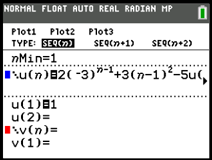
\includegraphics[width=0.48\linewidth]{gc/380863_lcd.png}\hfill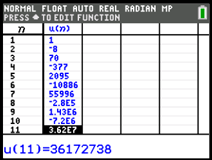
\includegraphics[width=0.48\linewidth]{gc/ce99e1_lcd.png}
\end{minipage}\par}
%% ============================================================ 4  SAJC 2025 P1 Q1
\defQ{4}{}{%
A function f is defined by $\mathrm{f}(x)=ax^{3}+bx^{2}+cx+d$ where $a$, $b$, $c$ and $d$ are constants. The graph of $y=\mathrm{f}(x)$ has a turning point at $x=-1$ and passes through the points $(2,10)$ and $(-2,-2)$. Given also that $\displaystyle\int_{-2}^{2}\mathrm{f}(x)\,\mathrm{d}x=16$, find the values of $a$, $b$, $c$ and $d$. \mk{4}
\src{SAJC 2025 Prelim P1 Q1}}
\defS{4}{%
\begin{topalign}
\mathrm{f}'(x)&=3ax^{2}+2bx+c\\
\mathrm{f}'(-1)&=0\\
3a-2b+c&=0 &&---(1)\\
\mathrm{f}(2)&=10\\
8a+4b+2c+d&=10 &&---(2)\\
\mathrm{f}(-2)&=-2\\
-8a+4b-2c+d&=-2 &&---(3)\\
\int_{-2}^{2}\big(ax^{3}+bx^{2}+cx+d\big)\,\mathrm{d}x&=16\\
\Big[\tfrac{a}{4}x^{4}+\tfrac{b}{3}x^{3}+\tfrac{c}{2}x^{2}+dx\Big]_{-2}^{2}&=16\\
(4a+\tfrac{8}{3}b+2c+2d)-(4a-\tfrac{8}{3}b+2c-2d)&=16\\
\tfrac{16}{3}b+4d&=16 &&---(4)
\end{topalign}
$\gcsys$\ $a=3,\ b=0,\ c=-9,\ d=4$}
%% ============================================================ 5  placeholder
\defQ{5}{}{%
The lines $l_{1}$ and $l_{2}$ have equations
\[\begin{aligned}
l_{1}:\ \mathbf{r}&=\begin{pmatrix}1\\2\\0\end{pmatrix}+\lambda\begin{pmatrix}-2\\1\\2\end{pmatrix},\\
l_{2}:\ \mathbf{r}&=\begin{pmatrix}0\\5\\-8\end{pmatrix}+\mu\begin{pmatrix}2\\-2\\3\end{pmatrix},
\end{aligned}\]
where $\lambda$ and $\mu$ are parameters.
\begin{qparts}
\pt{(i)} Show that $l_{1}$ and $l_{2}$ are skew lines. \mk{2}
\end{qparts}
\src{SAJC 2025 Prelim P1 Q3}}
\defS{5}{%
\begin{qparts}
\pt{(i)}
\begin{topalign}
1-2\lambda&=2\mu &&---(1)\\2+\lambda&=5-2\mu &&---(2)\\2\lambda&=-8+3\mu &&---(3)\\
\text{Solve (1) and (2): }\lambda&=-2,\ \mu=\tfrac52\\
&\text{Sub into (3):}\\
\text{LHS}&=2(-2)=-4\\
\text{RHS}&=-8+3\left(\tfrac52\right)=-\tfrac12\\
\text{LHS}&\neq\text{RHS},\ \text{no solution}\\
\therefore\ &l_{1}\text{ and }l_{2}\text{ do not intersect}\\
\because\ \begin{pmatrix}-2\\1\\2\end{pmatrix}&\neq k\begin{pmatrix}2\\-2\\3\end{pmatrix}\text{ for any } k\in\mathbb{R}\\
\therefore\ &l_{1}\text{ and }l_{2}\text{ are not parallel}\\
\therefore\ &l_{1}\text{ and }l_{2}\text{ are skew (shown)}
\end{topalign}
\end{qparts}}
%% ============================================================ 6  ACJC 2026 P1 Q1
\defQ{6}{}{%
Use an algebraic method to solve the inequalities
\[\frac{x(5x+9)}{x^{2}+2x+5}>x\geqslant3x-6.\] \mk{4}
\src{ACJC 2026 Prelim P1 Q1}}
\defS{6}{%
\begin{topalign}
x&\geqslant3x-6\\
x&\leqslant3 &&---(1)
\end{topalign}
\begin{topalign}
x^{2}+2x+5&=(x+1)^{2}+4>0\ \text{for all real } x
\end{topalign}
\begin{topalign}
\frac{x(5x+9)}{x^{2}+2x+5}&>x\\
5x^{2}+9x&>x(x^{2}+2x+5)\quad(\because x^{2}+2x+5>0)\\
x^{3}-3x^{2}-4x&<0\\
x(x-4)(x+1)&<0
\end{topalign}
\begin{center}\begin{tikzpicture}[x=1cm]
\draw[thin,-{Stealth[length=1.6mm]}](-3,0)--(3,0);
\foreach \p/\l in {-1.5/-1,0/0,1.5/4}{\draw(\p,0.1)--(\p,-0.1)node[below]{\small$\l$};}
\node at(-2.3,0.3){$-$};\node at(-0.75,0.3){$+$};\node at(0.75,0.3){$-$};\node at(2.3,0.3){$+$};
\end{tikzpicture}\end{center}
\begin{topalign}
x<-1\ \ \text{or}\ \ 0<x<4 &&---(2)
\end{topalign}
$(1)\cap(2):$\par
$\therefore\ x<-1\ \ \text{or}\ \ 0<x\leqslant3$}
%% ============================================================ 7  SAJC 2025 P2 Q1
\defQ{7}{}{%
\begin{qparts}
\pt{(i)} Solve the inequality $3\left|x^{2}-4\right|\leqslant\left|x+2\right|$. \mk{4}
\pt{(ii)} Hence, solve $\dfrac{3}{x^{2}}\left|1-4x^{2}\right|\leqslant\left|\dfrac{1+2x}{x}\right|$. \mk{2}
\end{qparts}
\src{SAJC 2025 Prelim P2 Q1}}
\defS{7}{%
\begin{qparts}
\pt{(i)} \begin{topalign}
3|x-2||x+2|&\leqslant|x+2|
\end{topalign}
$x=-2:\quad 0\leqslant0\ $ (true)\par
$x\neq-2:\ |x+2|>0$
\begin{topalign}
3|x-2|&\leqslant1\\
-\tfrac13\leqslant x-2&\leqslant\tfrac13\\
\tfrac53\leqslant x&\leqslant\tfrac73
\end{topalign}
$\therefore\ x=-2\ \ \text{or}\ \ \tfrac53\leqslant x\leqslant\tfrac73$
\pt{(ii)} \begin{topalign}
\frac{3}{x^{2}}\left|1-4x^{2}\right|&=3\left|\frac{1}{x^{2}}-4\right|\quad(\because x^{2}>0)\\
\left|\frac{1+2x}{x}\right|&=\left|\frac1x+2\right|\\
3\left|\Big(\frac1x\Big)^{2}-4\right|&\leqslant\left|\frac1x+2\right|\quad(x\to\tfrac1x)
\end{topalign}
\begin{topalign}
\frac1x=-2\ \ &\text{or}\ \ \frac53\leqslant\frac1x\leqslant\frac73
\end{topalign}
\begin{center}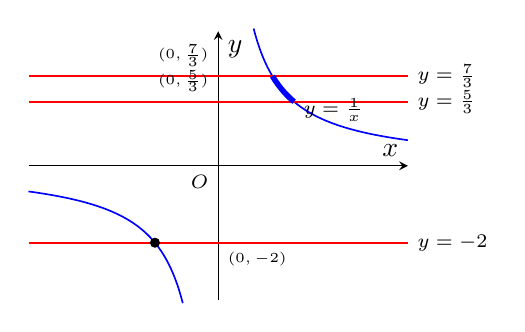
\begin{tikzpicture}
\begin{axis}[width=6.4cm,height=5cm,axis lines=middle,xmin=-1.5,xmax=1.5,ymin=-3.5,ymax=3.5,ticks=none,clip=false,xlabel=$x$,ylabel=$y$]
\addplot[blue,semithick,domain=0.28:1.5,samples=80]{1/x};
\addplot[blue,semithick,domain=-1.5:-0.28,samples=80]{1/x};
\addplot[red,semithick,domain=-1.5:1.5]{-2};\addplot[red,semithick,domain=-1.5:1.5]{5/3};\addplot[red,semithick,domain=-1.5:1.5]{7/3};\node[font=\scriptsize,anchor=north east] at (axis cs:0,0){$O$};\node[font=\tiny,anchor=north west] at (axis cs:0,-2){$(0,-2)$};\node[font=\tiny,anchor=south east] at (axis cs:0,5/3){$(0,\frac53)$};\node[font=\tiny,anchor=south east] at (axis cs:0,7/3){$(0,\frac73)$};
\addplot[blue,line width=2pt,domain=3/7:3/5]{1/x};\addplot[black,only marks,mark=*,mark size=1.6pt] coordinates{(-0.5,-2)};
\node[font=\scriptsize,anchor=west] at (axis cs:1.5,-2){$y=-2$};\node[font=\scriptsize,anchor=west] at (axis cs:1.5,5/3){$y=\frac53$};\node[font=\scriptsize,anchor=west] at (axis cs:1.5,7/3){$y=\frac73$};
\node[font=\scriptsize,anchor=south west] at (axis cs:0.6,0.9){$y=\frac1x$};
\end{axis}\end{tikzpicture}\end{center}
$\therefore\ x=-\tfrac12\ \ \text{or}\ \ \tfrac37\leqslant x\leqslant\tfrac35$
\end{qparts}}
%% ============================================================ 8  RVHS 2026 P1 Q2
\defQ{8}{}{%
\begin{qparts}
\pt{(a)} Solve the inequality $\left|\e^{x}-2\right|>\dfrac{1}{x^{2}-1}$ using a graphical approach. \mk{3}
\pt{(b)} Without the use of a graphing calculator, solve the inequality $\dfrac{x+2}{x-1}\geqslant\dfrac{2}{x-3}$. \mk{3}
\end{qparts}
\src{RVHS 2026 Prelim P1 Q2}}
\defS{8}{%
\begin{qparts}
\pt{(a)} \begin{center}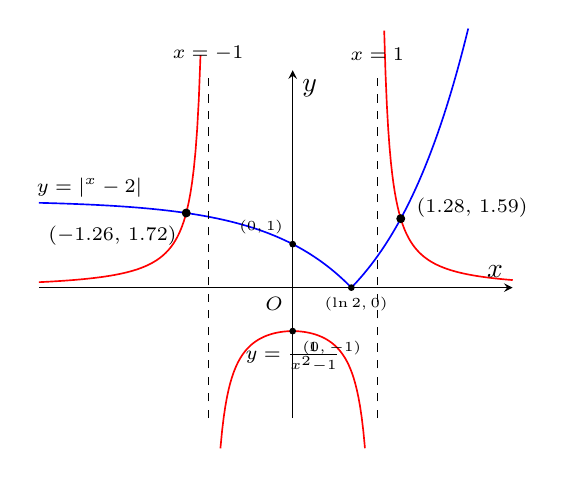
\begin{tikzpicture}
\begin{axis}[width=7.6cm,height=6cm,axis lines=middle,xmin=-3,xmax=2.6,ymin=-3,ymax=5,ticks=none,clip=false,xlabel=$x$,ylabel=$y$,restrict y to domain=-4:6]
\addplot[blue,semithick,domain=-3:2.1,samples=200]{abs(exp(x)-2)};
\addplot[red,semithick,domain=-3:-1.05,samples=100]{1/(x^2-1)};
\addplot[red,semithick,domain=-0.95:0.95,samples=100]{1/(x^2-1)};
\addplot[red,semithick,domain=1.05:2.6,samples=100]{1/(x^2-1)};\node[font=\scriptsize,anchor=north east] at (axis cs:0,0){$O$};\addplot[black,only marks,mark=*,mark size=1pt] coordinates{(0.6931,0)(0,1)(0,-1)};\node[font=\tiny,anchor=north] at (axis cs:0.75,0){$(\ln2,0)$};\node[font=\tiny,anchor=south east] at (axis cs:0,1){$(0,1)$};\node[font=\tiny,anchor=north west] at (axis cs:0,-1){$(0,-1)$};
\addplot[black,dashed,thin] coordinates{(-1,-3)(-1,5)};\addplot[black,dashed,thin] coordinates{(1,-3)(1,5)};
\addplot[black,only marks,mark=*,mark size=1.4pt] coordinates{(-1.258,1.716)(1.277,1.586)};
\node[font=\scriptsize,anchor=north east] at (axis cs:-1.258,1.65){$(-1.26,\,1.72)$};
\node[font=\scriptsize,anchor=south west] at (axis cs:1.35,1.4){$(1.28,\,1.59)$};
\node[font=\scriptsize] at (axis cs:-2.4,2.3){$y=|\e^{x}-2|$};
\node[font=\scriptsize] at (axis cs:0,-1.6){$y=\frac{1}{x^{2}-1}$};
\node[font=\scriptsize,anchor=south] at (axis cs:-1,5){$x=-1$};\node[font=\scriptsize,anchor=south] at (axis cs:1,5){$x=1$};
\end{axis}\end{tikzpicture}\end{center}
$\gcsys$\ intersections at $x=-1.2581$, $x=1.2770$\par
$\therefore\ x<-1.26\ \ \text{or}\ \ -1<x<1\ \ \text{or}\ \ x>1.28$
\pt{(b)} \begin{topalign}
\frac{x+2}{x-1}-\frac{2}{x-3}&\geqslant0\\
\frac{(x+2)(x-3)-2(x-1)}{(x-1)(x-3)}&\geqslant0\\
\frac{x^{2}-3x-4}{(x-1)(x-3)}&\geqslant0\\
\frac{(x-4)(x+1)}{(x-1)(x-3)}&\geqslant0
\end{topalign}
\begin{center}\begin{tikzpicture}[x=1cm]
\draw[thin,-{Stealth[length=1.6mm]}](-3.2,0)--(3.2,0);
\foreach \p/\l in {-1.8/-1,-0.6/1,0.6/3,1.8/4}{\draw(\p,0.1)--(\p,-0.1)node[below]{\small$\l$};}
\node at(-2.5,0.3){$+$};\node at(-1.2,0.3){$-$};\node at(0,0.3){$+$};\node at(1.2,0.3){$-$};\node at(2.5,0.3){$+$};
\end{tikzpicture}\end{center}
$\therefore\ x\leqslant-1\ \ \text{or}\ \ 1<x<3\ \ \text{or}\ \ x\geqslant4$
\end{qparts}}
%% ============================================================ 10  TJC 2022 P2 Q1
\defQ{10}{}{%
A movie theatre supports a charity event by providing discounted movie tickets at the following prices based on age group.
\begin{center}\renewcommand{\arraystretch}{1.15}
\begin{tabular}{|c|c|}\hline
Age group & Discounted ticket price\\\hline
$\leqslant12$ years & \$6\\\hline
13 to 49 years & \$9\\\hline
\begin{tabular}{@{}c@{}}$\geqslant50$ years\\(senior citizen)\end{tabular} & \$4\\\hline
\end{tabular}\end{center}
The event organiser plans to spend \$700 to sponsor 100 participants of which at least 35 of them are senior citizens. Find the possible number of participants for each age group. \mk{4}
\src{TJC 2022 Prelim P2 Q1}}
\defS{10}{%
Let $x$, $y$, $z$ be the number of participants aged $\leqslant12$, 13 to 49 and $\geqslant50$ years respectively.
\begin{topalign}
\left.\begin{aligned}x+y+z&=100 &&---(1)\\6x+9y+4z&=700 &&---(2)\end{aligned}\ \right\}&\ \Rightarrow\ \text{Using GC, } x=\tfrac{200}{3}-\tfrac53z,\ y=\tfrac{100}{3}+\tfrac23z\\
z&\geqslant35\\
\because\ x&\geqslant0\\
\tfrac{200}{3}-\tfrac53z&\geqslant0\\
z&\leqslant40\\
\therefore\ 35&\leqslant z\leqslant40
\end{topalign}
$x$, $y$, $z$ are non-negative integers. Using GC table:
\begin{topalign}
z=37&\Rightarrow x=5,\ y=58\\
z=40&\Rightarrow x=0,\ y=60\\
\therefore\ (x,y,z)&=(5,58,37)\ \text{or}\ (0,60,40)
\end{topalign}}
%% ============================================================ 11  SAJC 2019 P1 Q2
\defQ{11}{}{%
\begin{qparts}
\pt{(i)} On the same axes, sketch the curves with equations $y=\left|2x^{2}+6x+4\right|$ and $y=3-4x$, indicating any intercepts with the axes and points of intersection. Hence solve the inequality $3-4x<\left|2x^{2}+6x+4\right|$. \mk{4}
\pt{(ii)} Find the exact area bounded by the graphs of $y=3-4x$, $y=\left|2x^{2}+6x+4\right|$, $x=-3$ and $x=-1$. \mk{3}
\end{qparts}
\src{SAJC 2019 Prelim P1 Q2}}
\defS{11}{%
\begin{qparts}
\pt{(i)} \begin{center}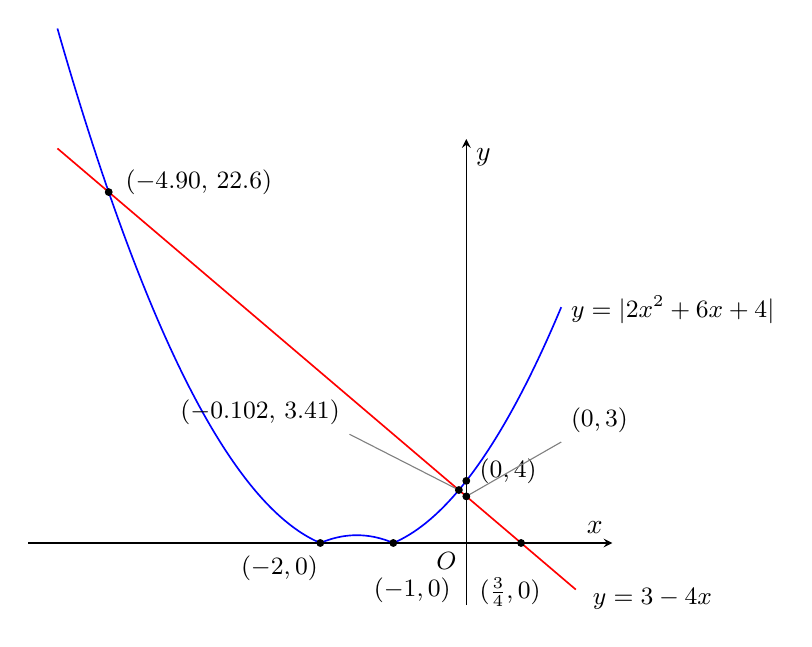
\begin{tikzpicture}
\begin{axis}[width=9cm,height=7.5cm,axis lines=middle,xmin=-6,xmax=2,ymin=-4,ymax=26,ticks=none,clip=false,xlabel=$x$,ylabel=$y$]
\addplot[blue,semithick,domain=-5.6:1.3,samples=300]{abs(2*x^2+6*x+4)};
\addplot[red,semithick,domain=-5.6:1.5]{3-4*x};
\addplot[black,only marks,mark=*,mark size=1.2pt] coordinates{(0,4)(0,3)(-2,0)(-1,0)(0.75,0)(-4.898,22.59)(-0.1021,3.408)};
\node[font=\small,anchor=north east] at (axis cs:0,0){$O$};
\node[font=\small,anchor=west] at (axis cs:0.05,4.6){$(0,4)$};
\draw[thin,gray] (axis cs:0,3)--(axis cs:1.3,6.5);\node[font=\small,anchor=south west] at (axis cs:1.3,6.5){$(0,3)$};
\node[font=\small,anchor=north east] at (axis cs:-1.9,-0.2){$(-2,0)$};
\node[font=\small,anchor=north west] at (axis cs:-1.4,-1.6){$(-1,0)$};
\node[font=\small,anchor=north] at (axis cs:0.6,-1.6){$(\frac34,0)$};
\node[font=\small,anchor=west] at (axis cs:-4.8,23.2){$(-4.90,\,22.6)$};
\draw[thin,gray] (axis cs:-0.1021,3.408)--(axis cs:-1.6,7);\node[font=\small,anchor=south east] at (axis cs:-1.6,7){$(-0.102,\,3.41)$};
\node[font=\small,anchor=west] at (axis cs:1.3,15){$y=|2x^{2}+6x+4|$};
\node[font=\small,anchor=west] at (axis cs:1.6,-3.6){$y=3-4x$};
\end{axis}\end{tikzpicture}\end{center}
\begin{topalign}
3-4x&=2x^{2}+6x+4\\
2x^{2}+10x+1&=0\\
x&=\frac{-5\pm\sqrt{23}}{2}\\
\therefore\ x&<\frac{-5-\sqrt{23}}{2}\ \ \text{or}\ \ x>\frac{-5+\sqrt{23}}{2}
\end{topalign}
\pt{(ii)}
\begin{topalign}
\text{Area}&=\int_{-3}^{-1}\left(3-4x-\left|2x^{2}+6x+4\right|\right)\mathrm{d}x\\
&=\int_{-3}^{-2}\left(3-4x-2x^{2}-6x-4\right)\mathrm{d}x+\int_{-2}^{-1}\left(3-4x+2x^{2}+6x+4\right)\mathrm{d}x\\
&=\int_{-3}^{-2}\left(-2x^{2}-10x-1\right)\mathrm{d}x+\int_{-2}^{-1}\left(2x^{2}+2x+7\right)\mathrm{d}x\\
&=\left[-\tfrac23x^{3}-5x^{2}-x\right]_{-3}^{-2}+\left[\tfrac23x^{3}+x^{2}+7x\right]_{-2}^{-1}\\
&=\left(\tfrac{16}{3}-20+2\right)-\left(18-45+3\right)+\left(-\tfrac23+1-7\right)-\left(-\tfrac{16}{3}+4-14\right)\\
&=20
\end{topalign}
\end{qparts}}
\defQ{9}{}{%
Solve the system of equations
\[\begin{aligned}
2x^{3}+3\ln y-\e^{z}&=18,\\
x^{3}-\ln y+2\e^{z}&=9,\\
x^{3}+2\ln y+\e^{z}&=11,
\end{aligned}\]
where $x$, $y$ and $z$ are real and $y>0$. \mk{4}
\src{Example}}
\defS{9}{%
\begin{topalign}
\text{Let } A=x^{3},\ B&=\ln y,\ C=\e^{z}\\
2A+3B-C&=18 &&---(1)\\
A-B+2C&=9 &&---(2)\\
A+2B+C&=11 &&---(3)
\end{topalign}
\topdisplay{\text{Using GC, } A=8,\ B=1,\ C=1}
\begin{topalign}
x^{3}&=8 &\ln y&=1 &\e^{z}&=1\\
\therefore\ x&=2 &\therefore\ y&=\e &\therefore\ z&=0
\end{topalign}}
%% ============================================================ 31  VJC 2025 Promo Q9(a),(b)
\defQ{31}{}{%
A curve $C$ has equation $y=\dfrac{x^{2}-4x+1}{x+1}$, $x\neq-1$.
\begin{qparts}
\pt{(a)} Prove, using an algebraic method, that $y=\dfrac{x^{2}-4x+1}{x+1}$ cannot lie between two certain values, to be determined in exact form. \mk{3}
\pt{(b)} Sketch $C$, stating the equations of any asymptotes, and the coordinates of any turning points and any axial intercepts. \mk{4}
\end{qparts}
\src{VJC 2025 Promo Q9(a), (b)}}
\defS{31}{%
\begin{gtpart}{(a)}{3}\begin{topalign}
y&=\frac{x^{2}-4x+1}{x+1}\\
yx+y&=x^{2}-4x+1\\
x^{2}+(-y-4)x+(1-y)&=0\\
\text{No real solution for }x:\quad(-y-4)^{2}-4(1-y)&<0\\
y^{2}+8y+16-4+4y&<0\\
y^{2}+12y+12&<0\\
(y+6)^{2}-24&<0\\
\left(y+6-\sqrt{24}\right)\left(y+6+\sqrt{24}\right)&<0\\
-6-2\sqrt6<y&<-6+2\sqrt6\\
\therefore\ y\text{ cannot lie between }&-6-2\sqrt6\ \text{and}\ -6+2\sqrt6
\end{topalign}\end{gtpart}
\begin{gtpart}{(b)}{4}\begin{topalign}
y&=x-5+\frac{6}{x+1}\\
\text{Asymptotes: }&x=-1,\ y=x-5\\
x=0:\ y&=1\\
y=0:\ x^{2}-4x+1=0\ \Rightarrow\ x&=0.268,\ 3.73\\
\text{Turning points: }&(1.45,-1.10),\ (-3.45,-10.9)
\end{topalign}
\begin{center}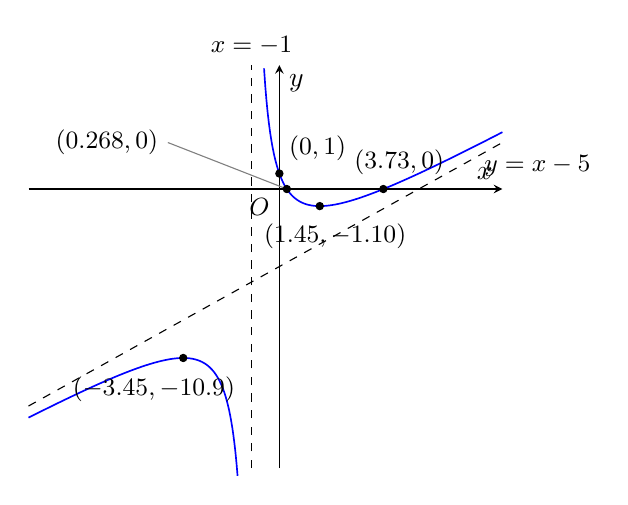
\begin{tikzpicture}
\begin{axis}[width=7.6cm,height=6.7cm,axis lines=middle,xmin=-9,xmax=8,ymin=-18,ymax=8,ticks=none,clip=false,xlabel=$x$,ylabel=$y$]
\addplot[black,dashed] coordinates{(-1,-18)(-1,8)};
\addplot[black,dashed,domain=-9:8]{x-5};
\addplot[blue,semithick,domain=-0.55:8,samples=200]{x-5+6/(x+1)};
\addplot[blue,semithick,domain=-9:-1.5,samples=200]{x-5+6/(x+1)};
\addplot[black,only marks,mark=*,mark size=1.3pt] coordinates{(0,1)(0.268,0)(3.73,0)(1.449,-1.101)(-3.449,-10.899)};
\node[font=\small,anchor=north east] at (axis cs:0,0){$O$};
\node[font=\small,anchor=south west] at (axis cs:0,1.2){$(0,1)$};
\node[font=\small,anchor=south] at (axis cs:4.3,0.3){$(3.73,0)$};
\draw[thin,gray] (axis cs:0.268,0)--(axis cs:-4,3);\node[font=\small,anchor=east] at (axis cs:-4,3){$(0.268,0)$};
\node[font=\small,anchor=north] at (axis cs:2,-1.6){$(1.45,-1.10)$};
\node[font=\small,anchor=north] at (axis cs:-4.5,-11.5){$(-3.45,-10.9)$};
\node[font=\small,anchor=south] at (axis cs:-1,8){$x=-1$};
\node[font=\small,anchor=west] at (axis cs:7,1.5){$y=x-5$};
\end{axis}\end{tikzpicture}\end{center}\end{gtpart}}
%% ============================================================ 32  SAJC 2025 Promo Q7
\defQ{32}{}{%
A curve $C$ has equation $y=ax+b+\dfrac{2b-a}{x+3}$, where $a$ and $b$ are constants such that $a>0$, $b\neq\dfrac12a$ and $x\neq-3$.
\begin{qparts}
\pt{(a)} If $C$ has no stationary points, use differentiation to find the relationship between $a$ and $b$. \mk{3}
\pt{(b)} It is now given that $b=a$.
\begin{qparts}
\pt{(i)} Find the $x$-coordinates of the turning points. \mk{2}
\pt{(ii)} Hence sketch $C$, stating the equations of any asymptotes and the coordinates of the axial intercepts and turning points. \mk{3}
\pt{(iii)} Verify that the point of intersection of the two asymptotes of $C$ lies on the line $y=kx+3k-2a$.\par
Hence, using the graph in part (b)(ii), find the range of values of $k$ in terms of $a$, such that the equation $x(k-a)+3k-2a-b-\dfrac{2b-a}{x+3}=0$ has real roots. \mk{2}
\end{qparts}
\end{qparts}
\src{SAJC 2025 Promo Q7}}
\defS{32}{%
\begin{qparts}
\pt{(a)} \begin{topalign}
\frac{\mathrm{d}y}{\mathrm{d}x}&=a-\frac{2b-a}{(x+3)^{2}}\\
\frac{\mathrm{d}y}{\mathrm{d}x}=0:\quad a-\frac{2b-a}{(x+3)^{2}}&=0\\
(x+3)^{2}&=\frac{2b-a}{a} &&---(1)\\
\text{No stationary points}\ \Rightarrow\ \frac{2b-a}{a}&<0\\
\text{Since }a>0,\quad 2b-a&<0\\
\therefore\ a&>2b
\end{topalign}
\pt{(b)(i)} \begin{topalign}
b=a:\quad (x+3)^{2}&=\frac{2a-a}{a}=1\\
x+3&=1\ \text{or}\ -1\\
x&=-2\ \text{or}\ -4
\end{topalign}
\pt{(b)(ii)} \begin{topalign}
y&=ax+a+\frac{a}{x+3}\\
\text{Asymptotes: }&x=-3,\ y=ax+a\\
x=-2:\ y=0;\quad x=-4:\ y&=-4a\\
\text{Turning points: }&(-2,0),\ (-4,-4a)\\
x=0:\ y&=\frac43a\\
y=0:\ ax+a+\frac{a}{x+3}=0\ \Rightarrow\ (x+1)(x+3)+1&=0\\
x^{2}+4x+4=0\ \Rightarrow\ (x+2)^{2}=0\ \Rightarrow\ x&=-2
\end{topalign}
\begin{center}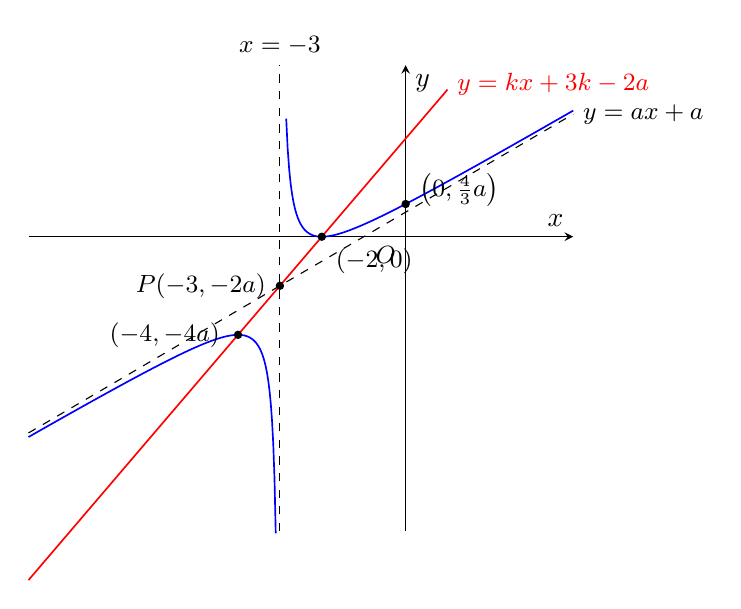
\begin{tikzpicture}
\begin{axis}[width=8.5cm,height=7.5cm,axis lines=middle,xmin=-9,xmax=4,ymin=-12,ymax=7,ticks=none,clip=false,xlabel=$x$,ylabel=$y$]
\addplot[black,dashed] coordinates{(-3,-12)(-3,7)};
\addplot[black,dashed,domain=-9:4]{x+1};
\addplot[blue,semithick,domain=-2.85:4,samples=200]{x+1+1/(x+3)};
\addplot[blue,semithick,domain=-9:-3.1,samples=200]{x+1+1/(x+3)};
\addplot[red,semithick,domain=-9:1]{2*(x+3)-2};
\addplot[black,only marks,mark=*,mark size=1.3pt] coordinates{(-2,0)(-4,-4)(0,1.333)(-3,-2)};
\node[font=\small,anchor=north east] at (axis cs:0,0){$O$};
\node[font=\small,anchor=north west] at (axis cs:-1.9,-0.1){$(-2,0)$};
\node[font=\small,anchor=east] at (axis cs:-4.2,-4){$(-4,-4a)$};
\node[font=\small,anchor=west] at (axis cs:0.1,1.9){$\left(0,\frac43a\right)$};
\node[font=\small,anchor=east] at (axis cs:-3.1,-2){$P(-3,-2a)$};
\node[font=\small,anchor=south] at (axis cs:-3,7){$x=-3$};
\node[font=\small,anchor=west] at (axis cs:4,5){$y=ax+a$};
\node[font=\small,anchor=west,red] at (axis cs:1,6.2){$y=kx+3k-2a$};
\end{axis}\end{tikzpicture}\end{center}
\pt{(b)(iii)} \begin{topalign}
x=-3\ \text{and}\ y=ax+a:\quad y&=-3a+a=-2a\\
\text{Intersection of asymptotes: }&P(-3,-2a)\\
x=-3:\quad \text{RHS}=k(-3)+3k-2a&=-2a=\text{LHS}\\
\therefore\ P\text{ lies on the line }&y=kx+3k-2a\\
x(k-a)+3k-2a-b-\frac{2b-a}{x+3}&=0\\
kx+3k-2a&=ax+b+\frac{2b-a}{x+3}\\
\text{Line through }P\text{ meets }C\ &\Rightarrow\ k>a
\end{topalign}
\end{qparts}}
%% ============================================================ 33  DHS 2025 Promo Q8
\defQ{33}{}{%
A curve $C$ has equation $\mathrm{f}(x)=\dfrac{3x^{2}+6x+k}{x+2}$, where $x>-2$ and $k$ is a non-zero real constant.\par
It is given that the function f is strictly increasing.
\begin{qparts}
\pt{(a)} Find the range of values of $k$. \mk{3}
\pt{(b)} Sketch the curve $C$, giving the coordinates of any points where $C$ crosses the $x$- and $y$-axes and the equations of any asymptotes. \mk{3}
\pt{(c)} By adding a suitable curve to the graph of the curve $C$ in (b), deduce the number of distinct real root(s) of the equation $\left(3x^{2}+6x+k\right)^{2}=\left(x^{2}+1\right)\left(9x^{2}+36x+36\right)$. \mk{3}
\end{qparts}
\src{DHS 2025 Promo Q8}}
\defS{33}{%
\begin{qparts}
\pt{(a)} \begin{topalign}
\mathrm{f}(x)&=\frac{3x^{2}+6x+k}{x+2}=3x+\frac{k}{x+2}\\
\mathrm{f}'(x)&=3-\frac{k}{(x+2)^{2}}=\frac{3x^{2}+12x+12-k}{(x+2)^{2}}\\
\text{f strictly increasing}\ \Rightarrow\ \mathrm{f}'(x)&>0\\
3x^{2}+12x+12-k&>0\quad\because\ (x+2)^{2}>0\ \text{for}\ x>-2\\
3(x+2)^{2}-k&>0\\
\text{Since }3(x+2)^{2}-k>-k\ \text{for all}\ x>-2,\quad -k&\geqslant0\\
k\neq0\ \Rightarrow\ k&<0
\end{topalign}
\pt{(b)} \begin{topalign}
y&=3x+\frac{k}{x+2}\\
\text{Asymptotes: }&y=3x,\ x=-2\\
x=0:\ y&=\frac{k}{2}\\
y=0:\ 3x^{2}+6x+k=0\ \Rightarrow\ x&=\frac{-6\pm\sqrt{36-12k}}{6}=-1\pm\frac{\sqrt{9-3k}}{3}\\
x>-2\ \Rightarrow\ x&=-1+\frac{\sqrt{9-3k}}{3}
\end{topalign}
\pt{(c)} \begin{topalign}
\left(3x^{2}+6x+k\right)^{2}&=\left(x^{2}+1\right)\left(9x^{2}+36x+36\right) &&---(*)\\
\left(3x^{2}+6x+k\right)^{2}&=9\left(x^{2}+1\right)(x+2)^{2}\\
\left(\frac{3x^{2}+6x+k}{x+2}\right)^{2}-9x^{2}&=9\\
\text{Draw the hyperbola }\ \frac{y^{2}}{3^{2}}-\frac{x^{2}}{1^{2}}&=1\\
\text{Asymptotes }y=\pm3x,\ \text{vertices }&(0,\pm3)
\end{topalign}
\begin{center}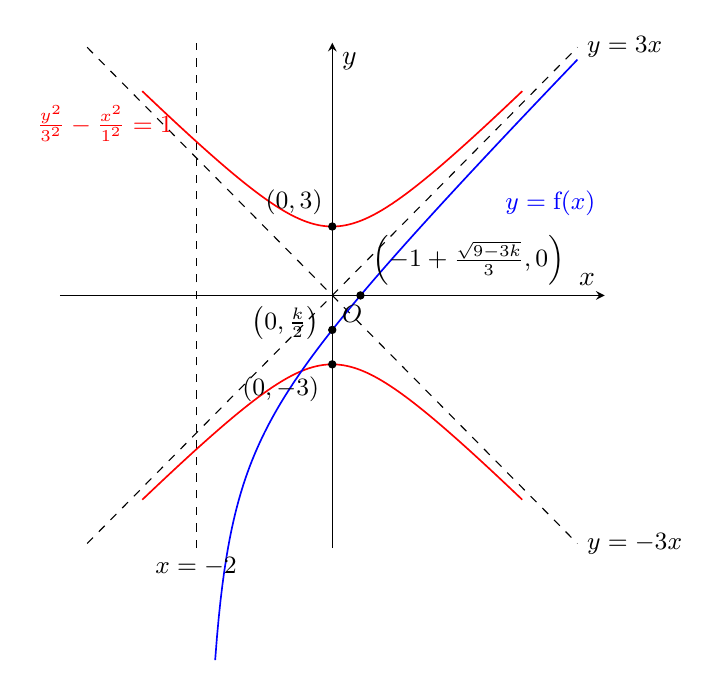
\begin{tikzpicture}
\begin{axis}[width=8.5cm,height=8cm,axis lines=middle,xmin=-4,xmax=4,ymin=-11,ymax=11,ticks=none,clip=false,xlabel=$x$,ylabel=$y$]
\addplot[black,dashed] coordinates{(-2,-11)(-2,11)};
\addplot[black,dashed,domain=-3.6:3.6]{3*x};
\addplot[black,dashed,domain=-3.6:3.6]{-3*x};
\addplot[red,semithick,domain=-1.75:1.75,samples=100,variable=\t]({sinh(t)},{3*cosh(t)});
\addplot[red,semithick,domain=-1.75:1.75,samples=100,variable=\t]({sinh(t)},{-3*cosh(t)});
\addplot[blue,semithick,domain=-1.72:3.6,samples=200]{3*x-3/(x+2)};
\addplot[black,only marks,mark=*,mark size=1.3pt] coordinates{(0,-1.5)(0.414,0)(0,3)(0,-3)};
\node[font=\small,anchor=north west] at (axis cs:0,0){$O$};
\node[font=\small,anchor=east] at (axis cs:-0.05,-1.2){$\left(0,\frac{k}{2}\right)$};
\node[font=\small,anchor=south west] at (axis cs:0.45,0){$\left(-1+\frac{\sqrt{9-3k}}{3},0\right)$};
\node[font=\small,anchor=south east] at (axis cs:0,3.1){$(0,3)$};
\node[font=\small,anchor=north east] at (axis cs:-0.05,-3.1){$(0,-3)$};
\node[font=\small,anchor=north] at (axis cs:-2,-11){$x=-2$};
\node[font=\small,anchor=west] at (axis cs:3.6,10.8){$y=3x$};
\node[font=\small,anchor=west] at (axis cs:3.6,-10.8){$y=-3x$};
\node[font=\small,anchor=west,blue] at (axis cs:2.4,4){$y=\mathrm{f}(x)$};
\node[font=\small,anchor=east,red] at (axis cs:-2.2,7.5){$\frac{y^{2}}{3^{2}}-\frac{x^{2}}{1^{2}}=1$};
\end{axis}\end{tikzpicture}\end{center}
\begin{topalign}
y=\mathrm{f}(x)\ \text{and}\ \frac{y^{2}}{3^{2}}-\frac{x^{2}}{1^{2}}=1\ &\text{have one intersection point}\\
\therefore\ (*)\ \text{has one real root}&
\end{topalign}
\end{qparts}}
%% ============================================================ 34  RVHS 2025 Prelim P1 Q12
\defQ{34}{}{%
The curve $C$ is defined by the parametric equations $x=6t-5$ and $y=2t^{2}+1$, where $t\geqslant\dfrac56$.
\begin{qparts}
\pt{(a)} Sketch the curve $C$, labelling the exact coordinates of any axial intercept(s). \mk{1}
\pt{(b)} Find the equation of the normal to $C$ at the point $P$ where $t=1$. \mk{2}
\pt{(c)} Find the acute angle between the normal to $C$ at the point $P$ where $t=1$ and the tangent to $C$ at the point $M$ where $t=3$. \mk{2}
\pt{(d)} The curve $C$ is translated 5 units in the positive $x$-direction and translated 3 units in the negative $y$-direction, to form the curve $D$. Find the equation of $D$ in parametric form. \mk{2}
\end{qparts}
The curve $E$ is defined by the parametric equations $x=7u$ and $y=\dfrac{9}{u}$, where $u\neq0$.
\begin{qparts}
\pt{(e)} Show that at the point of intersection of the curves $C$ and $E$, $6t^{3}-5t^{2}+3t-34=0$.
Deduce that there is only one point of intersection and find the coordinates of this point. \mk{4}
\end{qparts}
\src{RVHS 2025 Prelim P1 Q12}}
\defS{34}{%
\begin{qparts}
\pt{(a)} \begin{topalign}
t=\frac56:\quad x=6\left(\frac56\right)-5=0,\quad y=2\left(\frac56\right)^{2}+1&=\frac{43}{18}\\
\text{Endpoint (}y\text{-intercept): }&\left(0,\frac{43}{18}\right)
\end{topalign}
\begin{center}\begin{tikzpicture}
\begin{axis}[width=7cm,height=6cm,axis lines=middle,xmin=-10,xmax=22,ymin=-6,ymax=30,ticks=none,clip=false,xlabel=$x$,ylabel=$y$]
\addplot[red,semithick,domain=0.8333:3.6,samples=100,variable=\t]({6*t-5},{2*t^2+1});
\addplot[red,only marks,mark=*,mark size=1.4pt] coordinates{(0,2.389)};
\addplot[black,only marks,mark=*,mark size=1.3pt] coordinates{(7,9)};
\node[font=\small,anchor=north east] at (axis cs:0,0){$O$};
\node[font=\small,anchor=east] at (axis cs:-0.3,2.6){$\left(0,\frac{43}{18}\right)$};
\node[font=\small,anchor=west] at (axis cs:7.4,10){$(7,9)$};
\node[font=\small,red,anchor=west] at (axis cs:16.6,26){$C$};
\end{axis}\end{tikzpicture}\end{center}
\pt{(b)} \begin{topalign}
\frac{\mathrm{d}x}{\mathrm{d}t}=6,\quad \frac{\mathrm{d}y}{\mathrm{d}t}&=4t\\
\frac{\mathrm{d}y}{\mathrm{d}x}&=\frac{4t}{6}=\frac23t\\
t=1:\quad \frac{\mathrm{d}y}{\mathrm{d}x}=\frac23\ &\Rightarrow\ \text{gradient of normal}=-\frac32\\
t=1:\quad x=1,\ y&=3\\
y-3&=-\frac32(x-1)\\
y&=-\frac32x+\frac92
\end{topalign}
\pt{(c)} \begin{topalign}
t=3:\quad \text{gradient of tangent}&=\frac23(3)=2\\
\theta_{1}+\theta_{2}&=\tan^{-1}(2)-\tan^{-1}\left(-\frac32\right)=2.089942\ \text{or}\ 119.7^{\circ}\\
\text{Acute angle}&=\pi-2.089942\ \text{or}\ 180^{\circ}-119.7^{\circ}\\
&=1.05\ \text{or}\ 60.3^{\circ}
\end{topalign}
\pt{(d)} \begin{topalign}
x-5=6t-5\ &\Rightarrow\ x=6t\\
y+3=2t^{2}+1\ &\Rightarrow\ y=2t^{2}-2\\
D:\quad x=6t,\ y&=2t^{2}-2
\end{topalign}
\pt{(e)} \begin{topalign}
6t-5=7u\ \Rightarrow\ u&=\frac{6t-5}{7} &&---(1)\\
2t^{2}+1&=\frac{9}{u} &&---(2)\\
\text{Sub (1) into (2): }2t^{2}+1&=\frac{63}{6t-5}\\
\left(2t^{2}+1\right)(6t-5)&=63\\
12t^{3}-10t^{2}+6t-68&=0\\
6t^{3}-5t^{2}+3t-34&=0\quad\text{(shown)}\\
(t-2)\left(6t^{2}+7t+17\right)&=0\\
6t^{2}+7t+17:\ b^{2}-4ac=7^{2}-4(6)(17)&=-359<0\ \Rightarrow\ \text{no real roots}\\
\therefore\ t=2\ \text{only}\ \Rightarrow\ &\text{only one point of intersection}\\
t=2:\quad x=6(2)-5=7,\ y=2(2)^{2}+1&=9\\
\text{Point of intersection: }&(7,9)
\end{topalign}
\end{qparts}}
%% ============================================================ 35  HCI 2024 Promo Q12
\defQ{35}{}{%
The parametric equations of the curve $C$ are
\[x=\tan\theta-1\quad\text{and}\quad y=2\sec\theta,\quad\text{where }-\frac{\pi}{2}<\theta<\frac{\pi}{2}.\]
\begin{qparts}
\pt{(a)} Find $\dfrac{\mathrm{d}y}{\mathrm{d}x}$ in terms of $\theta$, leaving your answer in a single trigonometric function. \mk{2}
\pt{(b)} Find the equation of the tangent to $C$ at the point where it cuts the $y$-axis, leaving your answer in exact form. \mk{3}
\pt{(c)} Find the Cartesian equation of $C$. \mk{1}
\pt{(d)} Find the equations of the asymptotes and state the coordinates of any turning point(s). \mk{3}
\pt{(e)} The region bounded by the tangent found in part (b), the curve $C$ and the line $x=-1$ is rotated completely about the $x$-axis. Calculate the volume obtained. \mk{3}
\end{qparts}
\src{HCI 2024 Promo Q12}}
\defS{35}{%
\begin{qparts}
\pt{(a)} \begin{topalign}
\frac{\mathrm{d}y}{\mathrm{d}x}&=\frac{\mathrm{d}y}{\mathrm{d}\theta}\div\frac{\mathrm{d}x}{\mathrm{d}\theta}=\frac{2\sec\theta\tan\theta}{\sec^{2}\theta}=2\sin\theta
\end{topalign}
\pt{(b)} \begin{topalign}
x=0:\quad \tan\theta-1=0\ \Rightarrow\ \tan\theta&=1\\
\theta&=\frac{\pi}{4}\quad\text{since}\ -\frac{\pi}{2}<\theta<\frac{\pi}{2}\\
\theta=\frac{\pi}{4}:\quad y=\frac{2}{\cos\frac{\pi}{4}}=2\sqrt2,\quad \frac{\mathrm{d}y}{\mathrm{d}x}=2\sin\frac{\pi}{4}&=\sqrt2\\
\text{Tangent: }y&=\sqrt2x+2\sqrt2
\end{topalign}
\pt{(c)} \begin{topalign}
\tan^{2}\theta+1&=\sec^{2}\theta\\
(x+1)^{2}+1&=\left(\frac{y}{2}\right)^{2}\\
-\frac{\pi}{2}<\theta<\frac{\pi}{2}\ \Rightarrow\ 0<\cos\theta\leqslant1\ \Rightarrow\ \sec\theta\geqslant1\\
\therefore\ (x+1)^{2}+1=\left(\frac{y}{2}\right)^{2},\quad y&\geqslant2
\end{topalign}
\pt{(d)} \begin{topalign}
\text{Asymptotes: }\left(\frac{y}{2}\right)^{2}&=(x+1)^{2}\\
\frac{y}{2}&=\pm(x+1)\\
y=2x+2\quad\text{or}\quad y&=-2x-2\\
\text{Centre }(-1,0),\ y\geqslant2\ \Rightarrow\ &\text{turning point }(-1,2)
\end{topalign}
\begin{center}\begin{tikzpicture}
\begin{axis}[width=7cm,height=6.5cm,axis lines=middle,xmin=-4.5,xmax=2.5,ymin=-3,ymax=8,ticks=none,clip=false,xlabel=$x$,ylabel=$y$]
\addplot[black,dashed,domain=-4.5:2.5]{2*x+2};
\addplot[black,dashed,domain=-4.5:2.5]{-2*x-2};
\addplot[black,dashed] coordinates{(-1,-3)(-1,8)};
\addplot[red,semithick,domain=-1.1:2.2,samples=100]{sqrt(2)*x+2*sqrt(2)};
\addplot[blue,semithick,domain=-1.33:1.33,samples=150,variable=\t]({tan(deg(t))-1},{2/cos(deg(t))});
\fill[orange!60,opacity=0.6] (axis cs:-1,2)--plot[domain=-1:0,samples=30] (axis cs:\x,{2*sqrt((\x+1)^2+1)})--(axis cs:0,2.828)--(axis cs:-1,1.414)--cycle;
\addplot[black,only marks,mark=*,mark size=1.3pt] coordinates{(-1,2)(0,2.828)};
\node[font=\small,anchor=north east] at (axis cs:0,0){$O$};
\node[font=\small,anchor=east] at (axis cs:-1.2,2.3){$(-1,2)$};
\node[font=\small,anchor=west] at (axis cs:0.1,2.5){$\left(0,2\sqrt2\right)$};
\node[font=\small,anchor=south] at (axis cs:-1,8){$x=-1$};
\node[font=\small,anchor=west] at (axis cs:2.5,7){$y=2x+2$};
\node[font=\small,anchor=east] at (axis cs:-4.5,7){$y=-2x-2$};
\node[font=\small,anchor=west,red] at (axis cs:2.2,5.9){$y=\sqrt2x+2\sqrt2$};
\end{axis}\end{tikzpicture}\end{center}
\pt{(e)} \begin{topalign}
\frac{y^{2}}{4}&=(x+1)^{2}+1\\
y^{2}&=4(x+1)^{2}+4\\
\text{Volume}&=\pi\int_{-1}^{0}\left[4\left((x+1)^{2}+1\right)-\left(\sqrt2x+2\sqrt2\right)^{2}\right]\mathrm{d}x\\
&=2.09\ \text{units}^{3}
\end{topalign}
\end{qparts}}
\newenvironment{gtpartn}[1]{}{}
%% ============================================================ 41  NJC 2024 Promo Q4(b)
\defQ{41}{}{%
A curve with equation $y=\mathrm{h}(x)$ undergoes the following sequence of transformations.
\begin{center}\begin{tabular}{l}
\textbf{A}: A translation of 2 units in the positive direction of the $x$-axis.\\
\textbf{B}: A scaling parallel to the $x$-axis by factor of 3.\\
\textbf{C}: A reflection in the $y$-axis.
\end{tabular}\end{center}
The resultant curve has equation $y=-\dfrac{x^{2}}{6x+45}$. Find $\mathrm{h}(x)$. \mk{3}
\src{NJC 2024 Promo Q4(b)}}
\defS{41}{%
\begin{gtpart}{(b)}{3}\begin{topalign}
y&=-\frac{x^{2}}{6x+45}\\
&\text{C}^{-1}\text{: reflection in the $y$-axis }(x\to-x)\\
y&=-\frac{(-x)^{2}}{6(-x)+45}=-\frac{x^{2}}{-6x+45}\\
&\text{B}^{-1}\text{: scaling parallel to the $x$-axis by factor $\tfrac13$ }(x\to3x)\\
y&=-\frac{(3x)^{2}}{-6(3x)+45}=-\frac{9x^{2}}{-18x+45}=-\frac{x^{2}}{-2x+5}\\
&\text{A}^{-1}\text{: translation of 2 units in the negative $x$-direction }(x\to x+2)\\
y&=-\frac{(x+2)^{2}}{-2(x+2)+5}=-\frac{(x+2)^{2}}{-2x+1}\\
\mathrm{h}(x)&=\frac{(x+2)^{2}}{2x-1}
\end{topalign}\end{gtpart}}
%% ============================================================ 42  EJC 2025 Prelim P1 Q4
\defQ{42}{}{%
The diagram below shows the graph of $y=\mathrm{f}(2x)$. The graph has a turning point at $(2,0)$, and asymptotes with equations $x=0$ and $y=k$.
\begin{center}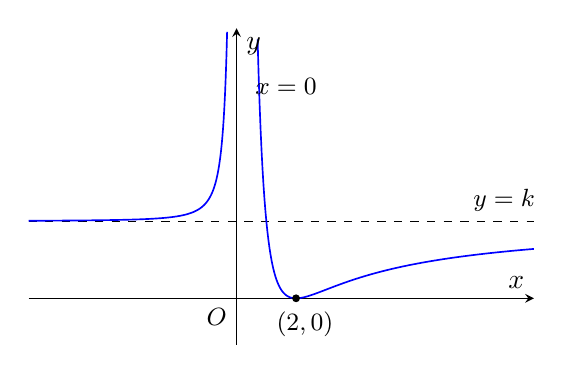
\begin{tikzpicture}
\begin{axis}[width=8cm,height=5.6cm,axis lines=middle,xmin=-7,xmax=10,ymin=-1.2,ymax=7,ticks=none,clip=false,restrict y to domain=-1.2:7,unbounded coords=jump,xlabel=$x$,ylabel=$y$]
\addplot[black,dashed,domain=-7:10]{2};
\addplot[blue,semithick,domain=-7:-0.04,samples=300]{2+0.5/x^2};
\addplot[blue,semithick,domain=0.04:10,samples=300]{2*(1-2/x)^2};
\addplot[black,only marks,mark=*,mark size=1.2pt] coordinates{(2,0)};
\node[font=\small,anchor=north east] at (axis cs:0,0){$O$};
\node[font=\small,anchor=north] at (axis cs:2.3,-0.1){$(2,0)$};
\node[font=\small,anchor=south] at (axis cs:9,2){$y=k$};
\node[font=\small,anchor=west] at (axis cs:0.3,5.5){$x=0$};
\end{axis}\end{tikzpicture}\end{center}
\begin{qparts}
\pt{(a)} State a single transformation that will transform the graph of $y=\mathrm{f}(2x)$ onto the graph of $y=\mathrm{f}(2x+4)$. Hence sketch the graph of $y=\mathrm{f}(2x+4)$. \mk{3}
\end{qparts}
On separate clearly labelled diagrams, sketch the graphs of
\begin{qparts}
\pt{(b)} $y=\dfrac{1}{\mathrm{f}(2x)}$, \mk{3}
\pt{(c)} $y=-\mathrm{f}(|x|)$. \mk{3}
\end{qparts}
\src{EJC 2025 Prelim P1 Q4}}
\defS{42}{%
\begin{gtpart}{(a)}{3}\fhl{Translation of 2 units in the negative $x$-direction.}\par\begin{center}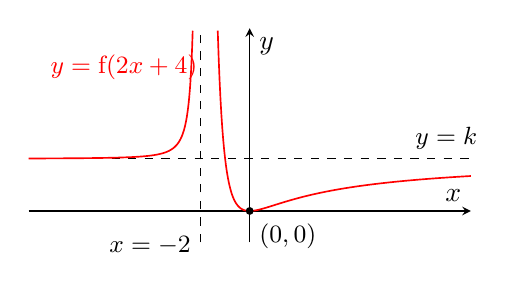
\begin{tikzpicture}
\begin{axis}[width=7.2cm,height=4.3cm,axis lines=middle,xmin=-9,xmax=9,ymin=-1.2,ymax=7,ticks=none,clip=false,restrict y to domain=-1.2:7,unbounded coords=jump,xlabel=$x$,ylabel=$y$]
\addplot[black,dashed,domain=-9:9]{2};
\addplot[black,dashed] coordinates{(-2,-1.2)(-2,7)};
\addplot[red,semithick,domain=-9:-2.04,samples=300]{2+0.5/(x+2)^2};
\addplot[red,semithick,domain=-1.96:9,samples=300]{2*(1-2/(x+2))^2};
\addplot[black,only marks,mark=*,mark size=1.2pt] coordinates{(0,0)};
\node[font=\small,anchor=north west] at (axis cs:0,-0.1){$(0,0)$};
\node[font=\small,anchor=south] at (axis cs:8,2){$y=k$};
\node[font=\small,anchor=north east] at (axis cs:-2,-0.6){$x=-2$};
\node[font=\small,red,anchor=west] at (axis cs:-8.5,5.5){$y=\mathrm{f}(2x+4)$};
\end{axis}\end{tikzpicture}\end{center}\end{gtpart}
\begin{gtpart}{(b)}{3}\begin{center}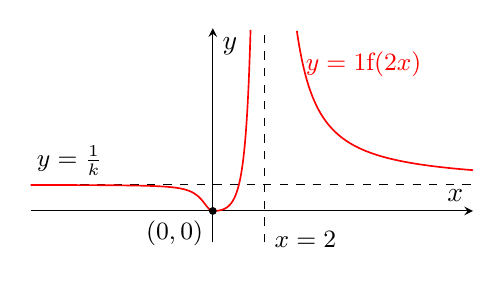
\begin{tikzpicture}
\begin{axis}[width=7.2cm,height=4.3cm,axis lines=middle,xmin=-7,xmax=10,ymin=-0.6,ymax=3.5,ticks=none,clip=false,restrict y to domain=-0.6:3.5,unbounded coords=jump,xlabel=$x$,ylabel=$y$]
\addplot[black,dashed,domain=-7:10]{0.5};
\addplot[black,dashed] coordinates{(2,-0.6)(2,3.5)};
\addplot[red,semithick,domain=-7:0,samples=300]{x^2/(2*x^2+0.5)};
\addplot[red,semithick,domain=0:1.97,samples=300]{x^2/(2*(x-2)^2)};
\addplot[red,semithick,domain=2.03:10,samples=300]{x^2/(2*(x-2)^2)};
\addplot[black,only marks,mark=*,mark size=1.2pt] coordinates{(0,0)};
\node[font=\small,anchor=north east] at (axis cs:0,0){$(0,0)$};
\node[font=\small,anchor=south] at (axis cs:-5.5,0.5){$y=\frac1k$};
\node[font=\small,anchor=north west] at (axis cs:2,-0.2){$x=2$};
\node[font=\small,red,anchor=west] at (axis cs:3.2,2.8){$y=\dfrac{1}{\mathrm{f}(2x)}$};
\end{axis}\end{tikzpicture}\end{center}\end{gtpart}
\begin{gtpart}{(c)}{3}\begin{center}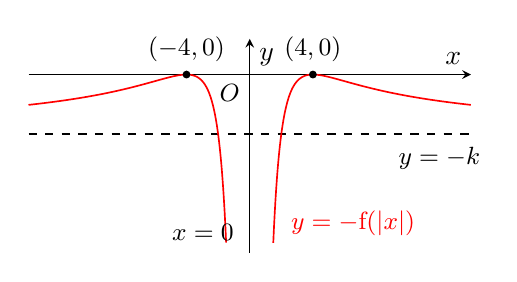
\begin{tikzpicture}
\begin{axis}[width=7.2cm,height=4.3cm,axis lines=middle,xmin=-14,xmax=14,ymin=-6,ymax=1.2,ticks=none,clip=false,restrict y to domain=-6:1.2,unbounded coords=jump,xlabel=$x$,ylabel=$y$]
\addplot[black,dashed,domain=-14:14]{-2};
\addplot[red,semithick,domain=0.3:14,samples=300]{-2*(1-4/x)^2};
\addplot[red,semithick,domain=-14:-0.3,samples=300]{-2*(1+4/x)^2};
\addplot[black,only marks,mark=*,mark size=1.2pt] coordinates{(4,0)(-4,0)};
\node[font=\small,anchor=south] at (axis cs:4,0.1){$(4,0)$};
\node[font=\small,anchor=south] at (axis cs:-4,0.1){$(-4,0)$};
\node[font=\small,anchor=north east] at (axis cs:0,0){$O$};
\node[font=\small,anchor=north] at (axis cs:12,-2.1){$y=-k$};
\node[font=\small,anchor=east] at (axis cs:-0.4,-5.3){$x=0$};
\node[font=\small,red,anchor=west] at (axis cs:2,-5){$y=-\mathrm{f}(|x|)$};
\end{axis}\end{tikzpicture}\end{center}\end{gtpart}}
%% ============================================================ 43  CJC 2025 Promo Q8
\defQ{43}{}{%
\mbox{}\par\vspace{-1ex}\begin{center}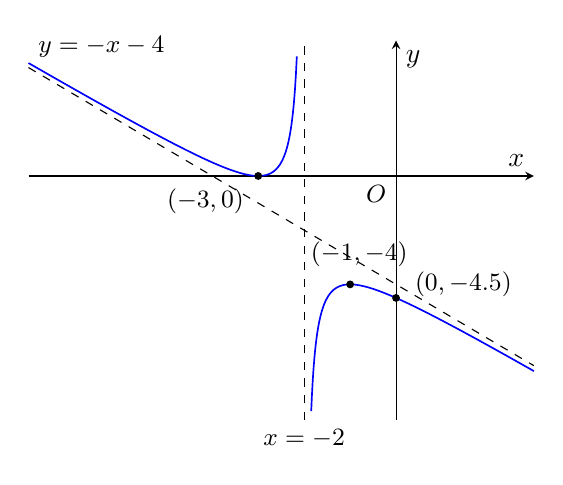
\begin{tikzpicture}
\begin{axis}[width=8cm,height=6.4cm,axis lines=middle,xmin=-8,xmax=3,ymin=-9,ymax=5,ticks=none,clip=false,restrict y to domain=-9:5,unbounded coords=jump,xlabel=$x$,ylabel=$y$]
\addplot[black,dashed] coordinates{(-2,-9)(-2,5)};
\addplot[black,dashed,domain=-8:3]{-x-4};
\addplot[blue,semithick,domain=-8:-2.02,samples=300]{-x-4-1/(x+2)};
\addplot[blue,semithick,domain=-1.98:3,samples=300]{-x-4-1/(x+2)};
\addplot[black,only marks,mark=*,mark size=1.2pt] coordinates{(-3,0)(-1,-4)(0,-4.5)};
\node[font=\small,anchor=north east] at (axis cs:0,0){$O$};
\node[font=\small,anchor=north east] at (axis cs:-3.1,-0.1){$(-3,0)$};
\node[font=\small,anchor=south] at (axis cs:-0.8,-3.7){$(-1,-4)$};
\node[font=\small,anchor=west] at (axis cs:0.2,-4){$(0,-4.5)$};
\node[font=\small,anchor=north] at (axis cs:-2,-9){$x=-2$};
\node[font=\small,anchor=south west] at (axis cs:-8,4){$y=-x-4$};
\end{axis}\end{tikzpicture}\end{center}
The diagram shows the curve $y=\mathrm{f}(x)$. The curve crosses the $x$-axis at its minimum point $(-3,0)$. It has a maximum turning point $(-1,-4)$ and crosses the $y$-axis at the point $(0,-4.5)$. The asymptotes of the curve are $x=-2$ and $y=-x-4$.\par
On separate diagrams, sketch the graphs of
\begin{qparts}
\pt{(a)} $y=\mathrm{f}'(x)$, \mk{3}
\pt{(b)} $y=\dfrac{1}{\mathrm{f}(x)}$, \mk{3}
\pt{(c)} $y=|\mathrm{f}(x)|$, \mk{3}
\end{qparts}
indicating the equations of any asymptotes, turning points and intersections with the axes.
\src{CJC 2025 Promo Q8}}
\defS{43}{%
\begin{gtpartn}{(a)}\begin{center}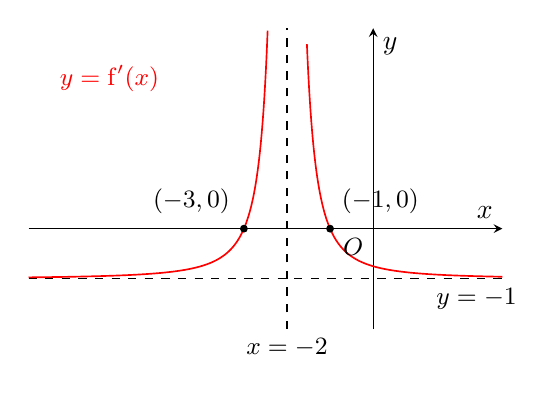
\begin{tikzpicture}
\begin{axis}[width=7.6cm,height=5.4cm,axis lines=middle,xmin=-8,xmax=3,ymin=-2,ymax=4,ticks=none,clip=false,restrict y to domain=-2:4,unbounded coords=jump,xlabel=$x$,ylabel=$y$]
\addplot[black,dashed] coordinates{(-2,-2)(-2,4)};
\addplot[black,dashed,domain=-8:3]{-1};
\addplot[red,semithick,domain=-8:-2.03,samples=300]{-1+1/(x+2)^2};
\addplot[red,semithick,domain=-1.97:3,samples=300]{-1+1/(x+2)^2};
\addplot[black,only marks,mark=*,mark size=1.2pt] coordinates{(-3,0)(-1,0)};
\node[font=\small,anchor=south east] at (axis cs:-3.1,0.1){$(-3,0)$};
\node[font=\small,anchor=south west] at (axis cs:-0.95,0.1){$(-1,0)$};
\node[font=\small,anchor=north east] at (axis cs:0,0){$O$};
\node[font=\small,anchor=north] at (axis cs:2.4,-1){$y=-1$};
\node[font=\small,anchor=north] at (axis cs:-2,-2){$x=-2$};
\node[font=\small,red,anchor=west] at (axis cs:-7.5,3){$y=\mathrm{f}'(x)$};
\end{axis}\end{tikzpicture}\end{center}\end{gtpartn}
\begin{gtpartn}{(b)}\begin{center}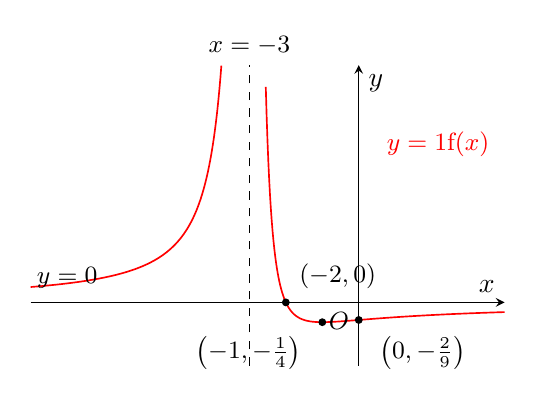
\begin{tikzpicture}
\begin{axis}[width=7.6cm,height=5.4cm,axis lines=middle,xmin=-9,xmax=4,ymin=-0.8,ymax=3,ticks=none,clip=false,restrict y to domain=-0.8:3,unbounded coords=jump,xlabel=$x$,ylabel=$y$]
\addplot[black,dashed] coordinates{(-3,-0.8)(-3,3)};
\addplot[red,semithick,domain=-9:-3.03,samples=300]{-(x+2)/(x+3)^2};
\addplot[red,semithick,domain=-2.97:4,samples=300]{-(x+2)/(x+3)^2};
\addplot[black,only marks,mark=*,mark size=1.2pt] coordinates{(-2,0)(-1,-0.25)(0,-0.2222)};
\node[font=\small,anchor=south west] at (axis cs:-1.9,0.05){$(-2,0)$};
\node[font=\small,anchor=north east] at (axis cs:-1.3,-0.3){$\left(-1,-\frac14\right)$};
\node[font=\small,anchor=north west] at (axis cs:0.3,-0.3){$\left(0,-\frac29\right)$};
\node[font=\small,anchor=north east] at (axis cs:0,0){$O$};
\node[font=\small,anchor=south] at (axis cs:-3,3){$x=-3$};
\node[font=\small,anchor=south] at (axis cs:-8,0.05){$y=0$};
\node[font=\small,red,anchor=west] at (axis cs:0.5,2){$y=\dfrac{1}{\mathrm{f}(x)}$};
\end{axis}\end{tikzpicture}\end{center}\end{gtpartn}
\begin{gtpartn}{(c)}\begin{center}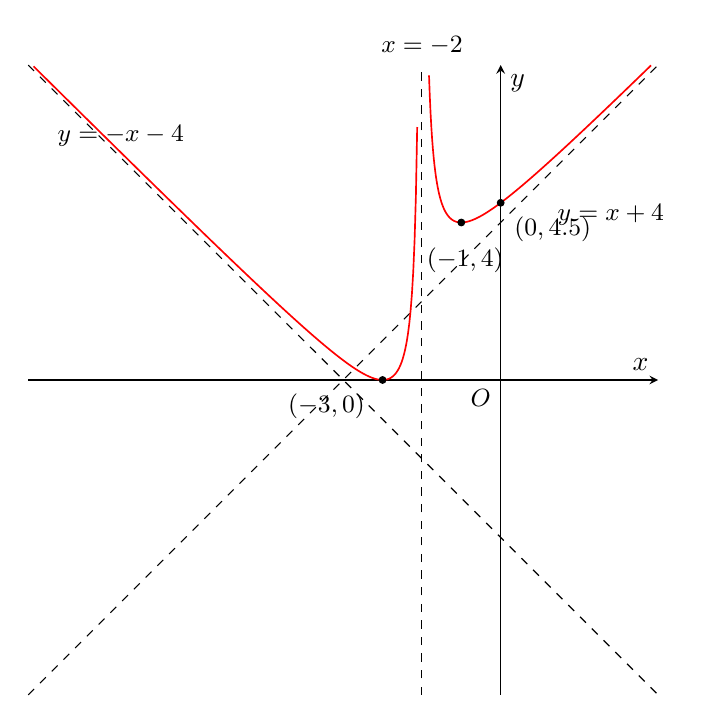
\begin{tikzpicture}
\begin{axis}[width=8cm,height=8cm,scale only axis,axis lines=middle,xmin=-12,xmax=4,ymin=-8,ymax=8,ticks=none,clip=false,restrict y to domain=-8:8,unbounded coords=jump,xlabel=$x$,ylabel=$y$]
\addplot[black,dashed] coordinates{(-2,-8)(-2,8)};
\addplot[black,dashed,domain=-12:4]{-x-4};
\addplot[black,dashed,domain=-12:4]{x+4};
\addplot[red,semithick,domain=-12:-2.02,samples=300]{abs(-x-4-1/(x+2))};
\addplot[red,semithick,domain=-1.98:4,samples=300]{abs(-x-4-1/(x+2))};
\addplot[black,only marks,mark=*,mark size=1.2pt] coordinates{(-3,0)(-1,4)(0,4.5)};
\node[font=\small,anchor=north east] at (axis cs:-3.2,-0.1){$(-3,0)$};
\node[font=\small,anchor=north] at (axis cs:-0.9,3.6){$(-1,4)$};
\node[font=\small,anchor=north west] at (axis cs:0.1,4.4){$(0,4.5)$};
\node[font=\small,anchor=north east] at (axis cs:0,0){$O$};
\node[font=\small,anchor=south] at (axis cs:-2,8){$x=-2$};
\node[font=\small,anchor=west] at (axis cs:-11.5,6.2){$y=-x-4$};
\node[font=\small,anchor=west] at (axis cs:1.2,4.2){$y=x+4$};
\end{axis}\end{tikzpicture}\end{center}\end{gtpartn}}
%% ============================================================ 44  RVHS 2026 Prelim P1 Q10(b)
\defQ{44}{}{%
Express $\dfrac{9x+5}{3x+2}$ in the form $a-\dfrac{b}{3x+2}$ where $a$ and $b$ are positive constants.\par
Hence, describe a sequence of transformations which transform the graph of $y=\dfrac{9x+5}{3x+2}$ to the graph of $y=\dfrac1x$. \mk{5}
\src{RVHS 2026 Prelim P1 Q10(b)}}
\defS{44}{%
\begin{gtpart}{(b)}{5}\begin{topalign}
\frac{9x+5}{3x+2}&=3-\frac{1}{3x+2}\qquad(a=3,\ b=1)\\
y=3-\frac{1}{3x+2}\ &\xrightarrow{\ y\to y+3\ }\ y=-\frac{1}{3x+2}\\
&\xrightarrow{\ y\to-y\ }\ y=\frac{1}{3x+2}\\
&\xrightarrow{\ x\to\frac x3\ }\ y=\frac{1}{x+2}\\
&\xrightarrow{\ x\to x-2\ }\ y=\frac1x
\end{topalign}
\begin{enumerate}\setlength\itemsep{0pt}
\item Translate 3 units in the negative $y$-direction
\item Reflect about the $x$-axis
\item Scale by factor 3 parallel to the $x$-axis
\item Translate 2 units in the positive $x$-direction
\end{enumerate}\end{gtpart}}
%% ============================================================ 51  2023 A-Level P1 Q7
\defQ{51}{}{%
The function f is defined by
\[\mathrm{f}:x\to\left|\frac{2x+4}{3-x}\right|,\qquad x\in\mathbb{R},\qquad x\neq3.\]
\begin{qparts}
\pt{(a)} Sketch the graph of $y=\mathrm{f}(x)$, giving the equations of any asymptotes and the coordinates of the points where the curve meets the axes. \mk{3}
\pt{(b)} Hence state the range of f. \mk{1}
\pt{(c)} Explain why the function $\mathrm{f}^{2}$ does not exist. \mk{1}
\end{qparts}
The domain of f is further restricted to $x\leqslant a$, where $a$ is a constant.
\begin{qparts}
\pt{(d)} State the greatest value of $a$ such that the function $\mathrm{f}^{-1}$ exists. \mk{1}
\pt{(e)} Hence find $\mathrm{f}^{-1}(x)$ and state its domain. \mk{4}
\end{qparts}
\src{2023 A-Level P1 Q7}}
\defS{51}{%
\begin{gtpart}{(a)}{3}\begin{topalign}
y=\left|\frac{2x+4}{3-x}\right|&=\left|-2+\frac{10}{3-x}\right|\\
\text{Asymptotes: }&y=|-2|=2,\quad x=3\\
x=0:\quad y&=\left|\frac43\right|=\frac43\\
y=0:\quad x&=-2
\end{topalign}
\begin{center}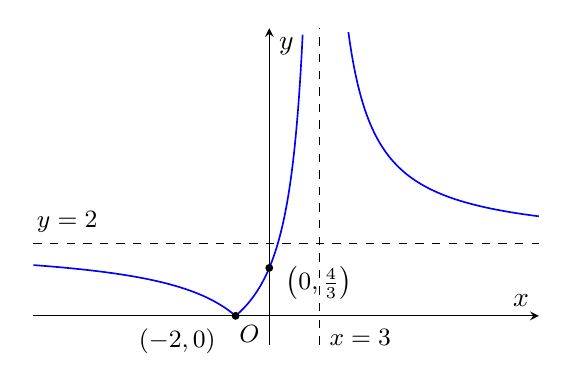
\begin{tikzpicture}
\begin{axis}[width=8cm,height=5.6cm,axis lines=middle,xmin=-14,xmax=16,ymin=-0.8,ymax=8,ticks=none,clip=false,restrict y to domain=-0.8:8,unbounded coords=jump,xlabel=$x$,ylabel=$y$]
\addplot[black,dashed,domain=-14:16]{2};
\addplot[black,dashed] coordinates{(3,-0.8)(3,8)};
\addplot[blue,semithick,domain=-14:2.96,samples=400]{abs((2*x+4)/(3-x))};
\addplot[blue,semithick,domain=3.04:16,samples=400]{abs((2*x+4)/(3-x))};
\addplot[black,only marks,mark=*,mark size=1.2pt] coordinates{(-2,0)(0,1.3333)};
\node[font=\small,anchor=north east] at (axis cs:-2.6,-0.1){$(-2,0)$};
\node[font=\small,anchor=north east] at (axis cs:0,0){$O$};
\node[font=\small,anchor=west] at (axis cs:0.4,0.9){$\left(0,\frac43\right)$};
\node[font=\small,anchor=south] at (axis cs:-12,2.05){$y=2$};
\node[font=\small,anchor=north west] at (axis cs:3,-0.1){$x=3$};
\end{axis}\end{tikzpicture}\end{center}\end{gtpart}
\begin{gtpart}{(b)}{1}\begin{topalign}
\mathrm{R}_{\mathrm f}&=[0,\infty)
\end{topalign}\end{gtpart}
\begin{gtpart}{(c)}{1}\begin{topalign}
\mathrm{R}_{\mathrm f}=[0,\infty),\quad \mathrm{D}_{\mathrm f}&=(-\infty,3)\cup(3,\infty)\\
3\in\mathrm{R}_{\mathrm f},\ 3\notin\mathrm{D}_{\mathrm f}\ &\Rightarrow\ \mathrm{R}_{\mathrm f}\not\subseteq\mathrm{D}_{\mathrm f}\\
\therefore\ \mathrm{f}^{2}&\text{ does not exist}
\end{topalign}\end{gtpart}
\begin{gtpart}{(d)}{1}\begin{topalign}
a&=-2
\end{topalign}
\end{gtpart}
\begin{gtpart}{(e)}{4}\begin{topalign}
x\leqslant-2:\quad\mathrm{f}(x)=\left|\frac{2x+4}{3-x}\right|&=-\frac{2x+4}{3-x}\\
\end{topalign}
\begin{center}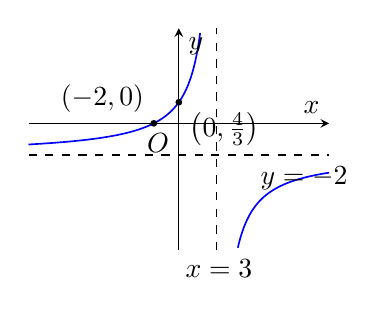
\begin{tikzpicture}[baseline]
\begin{axis}[width=5.4cm,height=4.4cm,axis lines=middle,xmin=-12,xmax=12,ymin=-8,ymax=6,ticks=none,clip=false,restrict y to domain=-8:6,unbounded coords=jump,xlabel=$x$,ylabel=$y$,every node/.append style={font=\scriptsize}]
\addplot[black,dashed] coordinates{(3,-8)(3,6)};
\addplot[black,dashed,domain=-12:12]{-2};
\addplot[blue,semithick,domain=-12:2.9,samples=200]{(2*x+4)/(3-x)};
\addplot[blue,semithick,domain=3.1:12,samples=200]{(2*x+4)/(3-x)};
\addplot[black,only marks,mark=*,mark size=1pt] coordinates{(-2,0)(0,1.333)};
\node[anchor=south east] at (axis cs:-2,0.1){$(-2,0)$};
\node[anchor=north west] at (axis cs:0.1,1.3){$\left(0,\frac43\right)$};
\node[anchor=north east] at (axis cs:0,0){$O$};
\node[anchor=north] at (axis cs:3.2,-8){$x=3$};
\node[anchor=north] at (axis cs:10,-2.1){$y=-2$};
\end{axis}\end{tikzpicture}\quad\raisebox{1.4cm}{$\Longrightarrow$}\quad
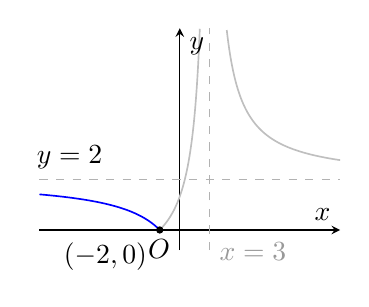
\begin{tikzpicture}[baseline]
\begin{axis}[width=5.4cm,height=4.4cm,axis lines=middle,xmin=-14,xmax=16,ymin=-0.8,ymax=8,ticks=none,clip=false,restrict y to domain=-0.8:8,unbounded coords=jump,xlabel=$x$,ylabel=$y$,every node/.append style={font=\scriptsize}]
\addplot[black!30,dashed,domain=-14:16]{2};
\addplot[black!30,dashed] coordinates{(3,-0.8)(3,8)};
\addplot[black!25,semithick,domain=-2:2.96,samples=300]{abs((2*x+4)/(3-x))};
\addplot[black!25,semithick,domain=3.04:16,samples=300]{abs((2*x+4)/(3-x))};
\addplot[blue,semithick,domain=-14:-2,samples=200]{abs((2*x+4)/(3-x))};
\addplot[black,only marks,mark=*,mark size=1.1pt] coordinates{(-2,0)};
\node[anchor=north east] at (axis cs:-2.3,-0.1){$(-2,0)$};
\node[anchor=north east] at (axis cs:0,0){$O$};
\node[anchor=south] at (axis cs:-11,2.05){$y=2$};
\node[black!40,anchor=north west] at (axis cs:3,-0.1){$x=3$};
\end{axis}\end{tikzpicture}\end{center}
\begin{topalign}
y&=\mathrm{f}(x)\\
-3y+xy&=2x+4\\
x(y-2)&=4+3y\\
x&=\frac{4+3y}{y-2}\\
\mathrm{f}^{-1}(x)&=\frac{4+3x}{x-2},\qquad \mathrm{D}_{\mathrm f^{-1}}=[0,2)
\end{topalign}\end{gtpart}}
%% ============================================================ 52  HCI 2025 Prelim P1 Q8
\defQ{52}{}{%
The function f is defined by
\[\mathrm{f}:x\mapsto\frac{ax-3}{5x-4},\ \text{for }x\in\mathbb{R},\ x\neq\frac45,\ \text{and }a\in\mathbb{R}.\]
\begin{qparts}
\pt{(a)} Find the range of f in terms of $a$. \mk{1}
\end{qparts}
The function f is such that $\mathrm{f}(x)=\mathrm{f}^{-1}(x)$ for all $x$ in the domain of f.
\begin{qparts}
\pt{(b)} Find the value of $a$. \mk{2}
\pt{(c)} Hence find $\mathrm{f}^{2025}(2)$. \mk{2}
\end{qparts}
Another function g is defined by
\[\mathrm{g}:x\mapsto\left(x-\frac15\right)^{2}+\frac25,\ \text{for }x\in\mathbb{R},\ 0<x<\frac35.\]
\begin{qparts}
\pt{(d)} Find the range of fg. \mk{2}
\end{qparts}
\src{HCI 2025 Prelim P1 Q8}}
\defS{52}{%
\begin{gtpart}{(a)}{1}\begin{topalign}
\text{Horizontal asymptote: }y&=\frac a5\\
\mathrm{R}_{\mathrm f}&=\mathbb{R}\setminus\left\{\frac a5\right\}
\end{topalign}\end{gtpart}
\begin{gtpart}{(b)}{2}\begin{topalign}
y&=\frac{ax-3}{5x-4}\\
5xy-4y&=ax-3\\
5xy-ax&=4y-3\\
x&=\frac{4y-3}{5y-a}\\
\mathrm{f}^{-1}(x)&=\frac{4x-3}{5x-a},\quad x\in\mathbb{R},\ x\neq\frac a5\\
\mathrm{f}(x)=\mathrm{f}^{-1}(x)\ &\Rightarrow\ a=4
\end{topalign}\end{gtpart}
\begin{gtpart}{(c)}{2}\begin{topalign}
\mathrm{f}^{-1}(x)=\mathrm{f}(x)\ &\Rightarrow\ \mathrm{f}^{2}(x)=\mathrm{f}\mathrm{f}^{-1}(x)=x\\
\mathrm{f}^{2025}(2)&=\mathrm{f}^{2}\big(\mathrm{f}^{2023}(2)\big)\\
&=\mathrm{f}^{2}\big(\mathrm{f}^{2021}(2)\big)\\
&=\cdots\\
&=\mathrm{f}(2)\\
&=\frac{4(2)-3}{5(2)-4}=\frac56
\end{topalign}\end{gtpart}
\begin{gtpart}{(d)}{2}\begin{topalign}
\mathrm{R}_{\mathrm g}&=\left[\frac25,\frac{14}{25}\right)\\
\mathrm{f}(x)&=\frac{4x-3}{5x-4}\\
\left(0,\frac35\right)\xrightarrow{\ \mathrm g\ }\left[\frac25,\frac{14}{25}\right)&\xrightarrow{\ \mathrm f\ }\left(\frac{19}{30},\frac7{10}\right]\\
\mathrm{R}_{\mathrm{fg}}&=\left(\frac{19}{30},\frac7{10}\right]
\end{topalign}
\begin{center}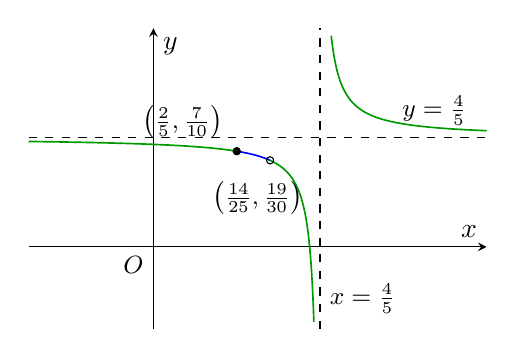
\begin{tikzpicture}
\begin{axis}[width=7.4cm,height=5.4cm,axis lines=middle,xmin=-0.6,xmax=1.6,ymin=-0.6,ymax=1.6,ticks=none,clip=false,restrict y to domain=-0.6:1.6,unbounded coords=jump,xlabel=$x$,ylabel=$y$]
\addplot[black,dashed,domain=-0.6:1.6]{0.8};
\addplot[black,dashed] coordinates{(0.8,-0.6)(0.8,1.6)};
\addplot[green!60!black,semithick,domain=-0.6:0.4,samples=100]{(4*x-3)/(5*x-4)};
\addplot[green!60!black,semithick,domain=0.56:0.79,samples=200]{(4*x-3)/(5*x-4)};
\addplot[green!60!black,semithick,domain=0.81:1.6,samples=200]{(4*x-3)/(5*x-4)};
\addplot[blue,semithick,domain=0.4:0.56,samples=60]{(4*x-3)/(5*x-4)};
\addplot[black,only marks,mark=*,mark size=1.3pt] coordinates{(0.4,0.7)};
\addplot[black,only marks,mark=o,mark size=1.3pt,fill=white] coordinates{(0.56,0.6333)};
\node[font=\small,anchor=north east] at (axis cs:0,0){$O$};
\node[font=\small,anchor=south east] at (axis cs:0.38,0.72){$\left(\frac25,\frac7{10}\right)$};
\node[font=\small,anchor=north] at (axis cs:0.5,0.55){$\left(\frac{14}{25},\frac{19}{30}\right)$};
\node[font=\small,anchor=south] at (axis cs:1.35,0.82){$y=\frac45$};
\node[font=\small,anchor=north west] at (axis cs:0.8,-0.2){$x=\frac45$};
\end{axis}\end{tikzpicture}\end{center}\end{gtpart}}
%% ============================================================ 53  VJC 2025 Prelim P1 Q5(a), (b)
\defQ{53}{}{%
The function f is given by
\[\mathrm{f}(x)=\begin{cases}2+\sqrt{2^{2}-(x-2)^{2}}, & 0<x\leqslant4,\\[1ex] 2-\sqrt{2^{2}-(x-6)^{2}}, & 4<x\leqslant8.\end{cases}\]
It is given that $\mathrm{f}(x)=\mathrm{f}(x+8)$ for all real values of $x$.
\begin{qparts}
\pt{(a)} On the diagram in the Printed Answer Book, sketch the graph of $y=\mathrm{f}(x)$ for $-6\leqslant x\leqslant7$, indicating clearly the coordinates of the end points and the points where the graph cuts the axes. \mk{3}
\pt{(b)} Without integrating, write down the exact area of the region bounded by $y=\mathrm{f}(x)$, the line $x=4$, the $x$-axis and the $y$-axis. \mk{1}
\end{qparts}
\src{VJC 2025 Prelim P1 Q5(a), (b)}}
\defS{53}{%
\begin{gtpart}{(a)}{3}{\color{gray}\small
\begin{minipage}[t]{0.48\linewidth}\centering
$\begin{aligned}y&=2+\sqrt{2^{2}-(x-2)^{2}}\\ y-2&=\sqrt{2^{2}-(x-2)^{2}}\\ (x-2)^{2}+(y-2)^{2}&=2^{2}\end{aligned}$\par
Centre $(2,2)$, radius 2.\par
Since it is a positive square root, it is the top half of this circle.
\end{minipage}\hfill
\begin{minipage}[t]{0.48\linewidth}\centering
$\begin{aligned}y&=2-\sqrt{2^{2}-(x-6)^{2}}\\ y-2&=-\sqrt{2^{2}-(x-6)^{2}}\\ (x-6)^{2}+(y-2)^{2}&=2^{2}\end{aligned}$\par
Centre $(6,2)$, radius 2.\par
Since it is a negative square root, it is the bottom half of this circle.
\end{minipage}\par}\vspace{-2mm}
\begin{center}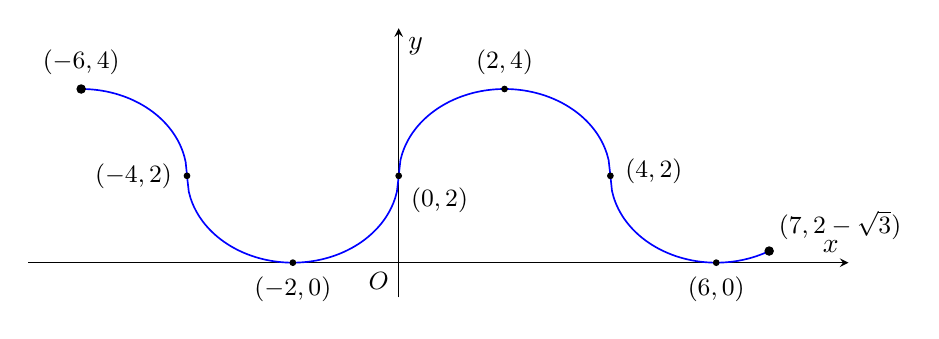
\begin{tikzpicture}
\begin{axis}[width=12cm,height=5cm,axis lines=middle,xmin=-7,xmax=8.5,ymin=-0.8,ymax=5.4,ticks=none,clip=false,restrict y to domain=-0.8:5.4,unbounded coords=jump,xlabel=$x$,ylabel=$y$]
\addplot[blue,semithick,domain=-6:-4,samples=80]{2+sqrt(max(0,4-(x+6)^2))};
\addplot[blue,semithick,domain=-4:0,samples=120]{2-sqrt(max(0,4-(x+2)^2))};
\addplot[blue,semithick,domain=0:4,samples=120]{2+sqrt(max(0,4-(x-2)^2))};
\addplot[blue,semithick,domain=4:7,samples=100]{2-sqrt(max(0,4-(x-6)^2))};
\addplot[black,only marks,mark=*,mark size=1.5pt] coordinates{(-6,4)(7,0.268)};
\addplot[black,only marks,mark=*,mark size=1pt] coordinates{(-4,2)(-2,0)(0,2)(2,4)(4,2)(6,0)};
\node[font=\small,anchor=south] at (axis cs:-6,4.1){$(-6,4)$};
\node[font=\small,anchor=east] at (axis cs:-4.1,2){$(-4,2)$};
\node[font=\small,anchor=north] at (axis cs:-2,-0.1){$(-2,0)$};
\node[font=\small,anchor=north west] at (axis cs:0.05,1.95){$(0,2)$};
\node[font=\small,anchor=south] at (axis cs:2,4.1){$(2,4)$};
\node[font=\small,anchor=west] at (axis cs:4.1,2.1){$(4,2)$};
\node[font=\small,anchor=north] at (axis cs:6,-0.1){$(6,0)$};
\node[font=\small,anchor=south west] at (axis cs:7,0.3){$(7,2-\sqrt3)$};
\node[font=\small,anchor=north east] at (axis cs:0,0){$O$};
\end{axis}\end{tikzpicture}\end{center}\end{gtpart}
\begin{gtpart}{(b)}{1}\begin{topalign}
\text{Area}&=2\times4+\frac12\pi\left(2^{2}\right)=8+2\pi
\end{topalign}\end{gtpart}}
%% ============================================================ 54  HCI 2024 Promo Q8
\defQ{54}{}{%
The function f is defined by
\[\mathrm{f}(x)=\begin{cases}2-\ln(x+\mathrm{e}) & \text{for }-\mathrm{e}<x<0,\\[1ex] \cos\left(\dfrac{\pi}{2}x\right) & \text{for }0\leqslant x\leqslant1.\end{cases}\]
\begin{qparts}
\pt{(a)} Given that the inverse function $\mathrm{f}^{-1}$ exists, find the exact value of $m$ if $\mathrm{f}^{-1}(m)=-1$. \mk{2}
\end{qparts}
Another function g is defined by
\[\mathrm{g}(x)=\sin x,\qquad\text{for }0\leqslant x\leqslant\frac{\pi}{4}.\]
\begin{qparts}
\pt{(b)} Explain why the composite function fg exists. \mk{2}
\pt{(c)} Find the exact value of $\mathrm{fg}\left(\dfrac{\pi}{6}\right)$. \mk{2}
\end{qparts}
The domain of f is further restricted to $0\leqslant x\leqslant1$.
\begin{qparts}
\pt{(d)} By considering $\mathrm{f}^{2}(1)$ and $\mathrm{f}^{3}(1)$, deduce the value(s) of $\mathrm{f}^{n}(1)$ where $n$ is a positive integer. \mk{2}
\end{qparts}
\src{HCI 2024 Promo Q8}}
\defS{54}{%
\begin{gtpart}{(a)}{2}\begin{topalign}
\mathrm{f}^{-1}(m)&=-1\\
m&=\mathrm{f}(-1)\\
&=2-\ln(\mathrm{e}-1)
\end{topalign}\end{gtpart}
\begin{gtpart}{(b)}{2}\begin{topalign}
\mathrm{R}_{\mathrm g}&=\left[0,\frac{1}{\sqrt2}\right]\\
\mathrm{D}_{\mathrm f}&=(-\mathrm{e},1]\\
\mathrm{R}_{\mathrm g}\subseteq\mathrm{D}_{\mathrm f}\ &\Rightarrow\ \mathrm{fg}\text{ exists}
\end{topalign}\end{gtpart}
\begin{gtpart}{(c)}{2}\begin{topalign}
\mathrm{fg}\left(\frac{\pi}{6}\right)&=\mathrm{f}\left(\frac12\right)\\
&=\cos\left(\frac{\pi}{4}\right)\\
&=\frac{1}{\sqrt2}
\end{topalign}\end{gtpart}
\begin{gtpart}{(d)}{2}
\begin{center}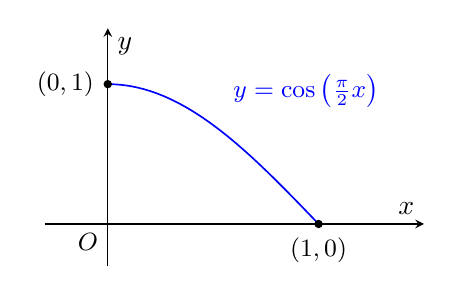
\begin{tikzpicture}
\begin{axis}[width=6.4cm,height=4.6cm,axis lines=middle,xmin=-0.3,xmax=1.5,ymin=-0.3,ymax=1.4,ticks=none,clip=false,restrict y to domain=-0.3:1.4,unbounded coords=jump,xlabel=$x$,ylabel=$y$]
\addplot[blue,semithick,domain=0:1,samples=80]{cos(deg(pi*x/2))};
\addplot[black,only marks,mark=*,mark size=1.3pt] coordinates{(0,1)(1,0)};
\node[font=\small,anchor=east] at (axis cs:-0.02,1){$(0,1)$};
\node[font=\small,anchor=north] at (axis cs:1,-0.03){$(1,0)$};
\node[font=\small,anchor=north east] at (axis cs:0,0){$O$};
\node[font=\small,blue,anchor=west] at (axis cs:0.55,0.95){$y=\cos\left(\frac{\pi}{2}x\right)$};
\end{axis}\end{tikzpicture}\end{center}
\begin{topalign}
\mathrm{f}^{2}(1)&=\mathrm{f}\big[\mathrm{f}(1)\big]=\mathrm{f}(0)=1\\
\mathrm{f}^{3}(1)&=\mathrm{f}\big[\mathrm{f}^{2}(1)\big]=\mathrm{f}(1)=0\\
\mathrm{f}^{n}(1)&=\begin{cases}0 & \text{if $n$ is odd}\\ 1 & \text{if $n$ is even}\end{cases}
\end{topalign}\end{gtpart}}
%% ============================================================ 55  ACJC 2022 Prelim P2 Q1
\defQ{55}{}{%
The function f is defined by
\[\mathrm{f}(x)=1-ax,\ x\in\mathbb{R},\ \text{where $a$ is a real constant.}\]
The function g is defined by
\[\mathrm{g}(x)=\begin{cases}x^{2}+3 & \text{for}\quad 0\leqslant x\leqslant2,\\ 7-x & \text{for}\quad 2<x\leqslant7.\end{cases}\]
\begin{qparts}
\pt{(i)} Find the set of possible values of $a$ such that $\mathrm{f}^{-1}$ exist. \mk{1}
\pt{(ii)} If $a=2$, describe a sequence of transformations that transform the graph of $y=\mathrm{g}(x)$ onto the graph of $y=\mathrm{fg}(x)$. \mk{3}
\pt{(iii)} The function gg is defined by
\[\mathrm{gg}(x)=\begin{cases}\mathrm{h}_1(x) & \text{for}\quad 0\leqslant x\leqslant2,\\ \mathrm{h}_2(x) & \text{for}\quad 2<x<5,\\ \mathrm{h}_3(x) & \text{for}\quad 5\leqslant x\leqslant7.\end{cases}\]
Find $\mathrm{h}_1(x)$, $\mathrm{h}_2(x)$ and $\mathrm{h}_3(x)$. \mk{3}
\end{qparts}
\src{ACJC 2022 Prelim P2 Q1}}
\defS{55}{%
\begin{gtpart}{(i)}{1}\begin{topalign}
a&\in\mathbb{R}\setminus\{0\}
\end{topalign}\end{gtpart}
\begin{gtpart}{(ii)}{3}\begin{topalign}
y=\mathrm{fg}(x)&=1-2\mathrm{g}(x)
\end{topalign}
Reflection of the graph of $y=\mathrm{g}(x)$ in the $x$-axis, followed by scaling by scale factor 2 parallel to the $y$-axis, followed by translation 1 unit in the positive $y$-direction.\par
\textbf{OR}\par
Translation of the graph of $y=\mathrm{g}(x)$ by $\frac12$ unit in the negative $y$-direction followed by reflection in the $x$-axis followed by scaling by scale factor 2 parallel to the $y$-axis.\par
\textbf{OR}\par
Translation of the graph of $y=\mathrm{g}(x)$ by $\frac12$ unit in the negative $y$-direction followed by scaling by scale factor 2 parallel to the $y$-axis followed by reflection in the $x$-axis.
\end{gtpart}
\begin{gtpart}{(iii)}{3}\begin{topalign}
\mathrm{gg}(x)&=\begin{cases}7-\left(x^{2}+3\right) & \text{for}\quad 0\leqslant x\leqslant2\\ 7-(7-x) & \text{for}\quad 2<x<5\\ (7-x)^{2}+3 & \text{for}\quad 5\leqslant x\leqslant7\end{cases}\\[1ex]
\therefore\ \mathrm{gg}(x)&=\begin{cases}4-x^{2} & \text{for}\quad 0\leqslant x\leqslant2\\ x & \text{for}\quad 2<x<5\\ x^{2}-14x+52 & \text{for}\quad 5\leqslant x\leqslant7\end{cases}
\end{topalign}\end{gtpart}}
%% ============================================================ 56  CJC 2025 Prelim P2 Q2(a), (b)
\defQ{56}{}{%
Functions f and g are defined by
\[\mathrm{f}:x\to\frac{4}{(x-4)^{2}},\quad x\in\mathbb{R},\ x\neq4,\]
\[\mathrm{g}:x\to\ln\left(1+\frac1x\right),\quad x\in\mathbb{R},\ x>0.\]
\begin{qparts}
\pt{(a)} Sketch the graph of $y=\mathrm{f}(x)$, stating the equations of any asymptotes, the coordinates of the points where it crosses the axes and the coordinates of the turning points, if any. \mk{2}
\pt{(b)} Show that gf exists. Hence find the rule, domain and range of gf. \mk{4}
\end{qparts}
\src{CJC 2025 Prelim P2 Q2(a), (b)}}
\defS{56}{%
\begin{gtpart}{(a)}{2}
\begin{center}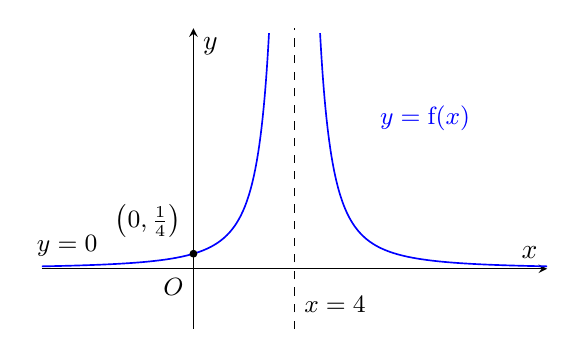
\begin{tikzpicture}
\begin{axis}[width=8cm,height=5.4cm,axis lines=middle,xmin=-6,xmax=14,ymin=-1,ymax=4,ticks=none,clip=false,restrict y to domain=-1:4,unbounded coords=jump,xlabel=$x$,ylabel=$y$]
\addplot[black,dashed] coordinates{(4,-1)(4,4)};
\addplot[blue,semithick,domain=-6:3.02,samples=300]{4/(x-4)^2};
\addplot[blue,semithick,domain=4.98:14,samples=300]{4/(x-4)^2};
\addplot[black,only marks,mark=*,mark size=1.2pt] coordinates{(0,0.25)};
\node[font=\small,anchor=south east] at (axis cs:-0.1,0.35){$\left(0,\frac14\right)$};
\node[font=\small,anchor=north east] at (axis cs:0,0){$O$};
\node[font=\small,anchor=south] at (axis cs:-5,0.05){$y=0$};
\node[font=\small,anchor=north west] at (axis cs:4,-0.3){$x=4$};
\node[font=\small,blue,anchor=west] at (axis cs:7,2.5){$y=\mathrm{f}(x)$};
\end{axis}\end{tikzpicture}\end{center}\end{gtpart}
\begin{gtpart}{(b)}{4}
For gf to exist, $\mathrm{R}_{\mathrm f}\subseteq\mathrm{D}_{\mathrm g}$,
\begin{topalign}
\mathrm{R}_{\mathrm f}&=(0,\infty)\\
\mathrm{D}_{\mathrm g}&=(0,\infty)
\end{topalign}
Since $\mathrm{R}_{\mathrm f}\subseteq\mathrm{D}_{\mathrm g}$, gf exists (shown)
\begin{topalign}
\mathrm{gf}(x)&=\mathrm{g}\left[\frac{4}{(x-4)^{2}}\right]\\
&=\ln\left[1+\left(\frac{1}{\frac{4}{(x-4)^{2}}}\right)\right]\\
&=\ln\left[1+\frac{(x-4)^{2}}{4}\right]\\
\mathrm{D}_{\mathrm{gf}}=\mathrm{D}_{\mathrm f}&=(-\infty,4)\cup(4,\infty)
\end{topalign}
OR
\begin{topalign}
\mathrm{D}_{\mathrm{gf}}=\mathrm{D}_{\mathrm f}&=\mathbb{R}\setminus\{4\}
\end{topalign}
\textbf{\underline{Method 1: Mapping}}
\[\mathrm{D}_{\mathrm f}=(-\infty,4)\cup(4,\infty)\xrightarrow{\ \mathrm f\ }\mathrm{R}_{\mathrm f}=(0,\infty)\xrightarrow{\ \mathrm g\ }\mathrm{R}_{\mathrm{gf}}=(0,\infty)\]
\begin{center}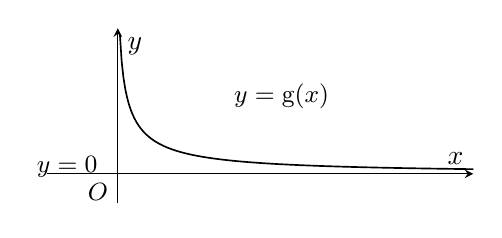
\begin{tikzpicture}
\begin{axis}[width=7cm,height=3.8cm,axis lines=middle,xmin=-2,xmax=10,ymin=-0.6,ymax=3,ticks=none,clip=false,xlabel=$x$,ylabel=$y$,restrict y to domain=-0.6:3]
\addplot[black,semithick,domain=0.06:10,samples=200]{ln(1+1/x)};
\node[font=\small,anchor=north east] at (axis cs:0,0){$O$};
\node[font=\small,anchor=east] at (axis cs:-0.3,0.15){$y=0$};
\node[font=\small,anchor=west] at (axis cs:3,1.6){$y=\mathrm{g}(x)$};
\end{axis}\end{tikzpicture}\end{center}
\textbf{\underline{Method 2: Sketch $y=\mathrm{gf}(x)$ for given domain}}
\begin{center}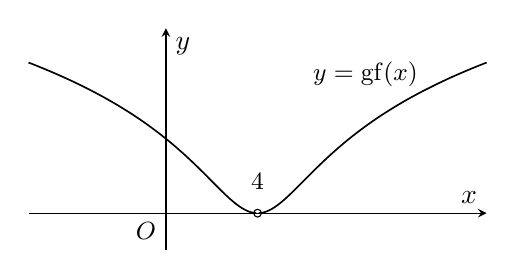
\begin{tikzpicture}
\begin{axis}[width=7.4cm,height=4.4cm,axis lines=middle,xmin=-6,xmax=14,ymin=-0.8,ymax=4,ticks=none,clip=false,xlabel=$x$,ylabel=$y$]
\addplot[black,semithick,domain=-6:3.95,samples=200]{ln(1+(x-4)^2/4)};
\addplot[black,semithick,domain=4.05:14,samples=200]{ln(1+(x-4)^2/4)};
\addplot[black,only marks,mark=o,mark size=1.4pt,fill=white] coordinates{(4,0)};
\node[font=\small,anchor=south] at (axis cs:4,0.3){$4$};
\node[font=\small,anchor=north east] at (axis cs:0,0){$O$};
\node[font=\small,anchor=west] at (axis cs:6,3){$y=\mathrm{gf}(x)$};
\end{axis}\end{tikzpicture}\end{center}
\begin{topalign}
\mathrm{R}_{\mathrm{gf}}&=(0,\infty)
\end{topalign}
\end{gtpart}}
%% ============================================================ 57  2016 A-Level P1 Q10(b)
\defQ{57}{}{%
\fhlp{The function $\mathrm{g}$, with domain the set of non-negative integers, is given by
\[\mathrm{g}(n)=\begin{cases}1&\text{for }n=0,\\2+\mathrm{g}\left(\tfrac12n\right)&\text{for }n\text{ even},\\1+\mathrm{g}(n-1)&\text{for }n\text{ odd}.\end{cases}\]}
\begin{qparts}
\pt{(i)} \fhl{Find $\mathrm{g}(4)$, $\mathrm{g}(7)$ and $\mathrm{g}(12)$.} \mk{\fhl{3}}
\pt{(ii)} Does $\mathrm{g}$ have an inverse? Justify your answer. \mk{\fhl{2}}
\end{qparts}
\src{2016 A-Level P1 Q10(b)}}
\defS{57}{%
\begin{gtpart}{(i)}{3}\fhlp{$\begin{aligned}[t]
\mathrm{g}(4)&=2+\mathrm{g}\left(\tfrac12\times4\right)=2+\mathrm{g}(2)=2+\left[2+\mathrm{g}\left(\tfrac12\times2\right)\right]=4+\mathrm{g}(1)\\
&=4+\left[1+\mathrm{g}(1-1)\right]=5+\mathrm{g}(0)=5+1=6\\[1ex]
\mathrm{g}(7)&=1+\mathrm{g}(7-1)=1+\mathrm{g}(6)=1+\left[2+\mathrm{g}\left(\tfrac12\times6\right)\right]=3+\mathrm{g}(3)\\
&=3+\left[1+\mathrm{g}(3-1)\right]=4+\mathrm{g}(2)=4+\left[2+\mathrm{g}\left(\tfrac12\times2\right)\right]=6+\mathrm{g}(1)\\
&=6+\left[1+\mathrm{g}(1-1)\right]=7+\mathrm{g}(0)=7+1=8\\[1ex]
\mathrm{g}(12)&=2+\mathrm{g}\left(\tfrac12\times12\right)=2+\mathrm{g}(6)=2+\left[2+\mathrm{g}\left(\tfrac12\times6\right)\right]=4+\mathrm{g}(3)\\
&=4+\left[1+\mathrm{g}(3-1)\right]=5+\mathrm{g}(2)=5+\left[2+\mathrm{g}\left(\tfrac12\times2\right)\right]=7+\mathrm{g}(1)\\
&=7+\left[1+\mathrm{g}(1-1)\right]=8+\mathrm{g}(0)=8+1=9
\end{aligned}$}\par\smallskip
\fhl{{\footnotesize Solution source: Achevas (Jack Ng), ``A-Level H2 Maths 2016 -- Paper 1'', www.achevas.com.}}\end{gtpart}
\begin{gtpart}{(ii)}{2}\fhlp{$\begin{aligned}[t]
\mathrm{g}(5)&=1+\mathrm{g}(4)=1+6=7\\
\mathrm{g}(6)&=2+\mathrm{g}(3)=2+\left[1+\mathrm{g}(2)\right]=3+\mathrm{g}(2)\\
&=3+\left[2+\mathrm{g}(1)\right]=5+\mathrm{g}(1)=5+\left[1+\mathrm{g}(0)\right]=6+1=7
\end{aligned}$}\par\smallskip
\fhl{Since $\mathrm{g}(5)=\mathrm{g}(6)$, $\mathrm{g}$ does not have an inverse.}\end{gtpart}}
\providecommand{\gcph}[1]{\par\noindent\fbox{\parbox{0.6\textwidth}{\centering\small\color{red}[GC SCREEN PLACEHOLDER] #1}}\par\smallskip}
%% ============================================================ 61  JPJC 2025 Prelim P1 Q8(b)
\defQ{61}{}{%
It is given $\displaystyle\sum_{r=1}^{n}r^{3}=\frac{n^{2}(n+1)^{2}}{4}$ and $u_r=2r^{3}+5$.
\begin{qparts}
\pt{(i)} Find $\displaystyle\sum_{r=1}^{n}u_r$. \mk{2}
\pt{(ii)} Hence, or otherwise, find $\displaystyle\sum_{r=2}^{n}\left(2(r+2)^{3}+5\right)$. \mk{3}
\pt{(iii)} Explain why the series $\displaystyle\sum_{r=1}^{\infty}u_r$ does not converge. \mk{1}
\end{qparts}
\src{JPJC 2025 Prelim P1 Q8(b)}}
\defS{61}{%
\begin{gtpart}{(i)}{2}\begin{topalign}
\sum_{r=1}^{n}\left(2r^{3}+5\right)&=2\sum_{r=1}^{n}r^{3}+\sum_{r=1}^{n}5\\&=2\left(\frac{n^{2}(n+1)^{2}}{4}\right)+5n\\&=\frac{n^{2}(n+1)^{2}}{2}+5n
\end{topalign}\end{gtpart}
\begin{gtpart}{(ii)}{3}\begin{topalign}
\sum_{r=2}^{n}\left(2(r+2)^{3}+5\right)&=\left(2(2+2)^{3}+5\right)+\dots+\left(2(n+2)^{3}+5\right)\\&=\sum_{r=4}^{n+2}\left(2r^{3}+5\right)\\&=\sum_{r=1}^{n+2}\left(2r^{3}+5\right)-\sum_{r=1}^{3}\left(2r^{3}+5\right)\\&=\frac{(n+2)^{2}(n+3)^{2}}{2}+5(n+2)-\left[\left(\frac{3^{2}(4)^{2}}{2}\right)+5(3)\right]\\&=\frac{(n+2)^{2}(n+3)^{2}}{2}+5n-77
\end{topalign}\end{gtpart}
\begin{gtpart}{(iii)}{1}\begin{topalign}
\text{From (i) }\sum_{r=1}^{n}u_r&=\frac{n^{2}(n+1)^{2}}{2}+5n\\\text{As }n\to\infty,\ \frac{n^{2}(n+1)^{2}}{2}&\to\infty,\quad5n\to\infty
\end{topalign}
Hence, $\displaystyle\sum_{r=1}^{n}u_r=\frac{n^{2}(n+1)^{2}}{2}+5n\to\infty$, series $\displaystyle\sum_{r=1}^{\infty}u_r$ does not converge.\end{gtpart}}
%% ============================================================ 62  VJC 2025 Prelim P1 Q6(a), (b), (d)
\defQ{62}{}{%
It is given that $\displaystyle\sum_{r=2}^{n}\frac{1}{r\left(r^{2}-1\right)}=\frac14+\frac{1}{2(n+1)}-\frac{1}{2n}$.
\begin{qparts}
\pt{(a)} Show that $\displaystyle\sum_{r=2}^{n}\frac{1}{r\left(r^{2}-1\right)}$ is less than $\frac14$. \mk{2}
\pt{(b)} Give a reason why the series $\displaystyle\sum_{r=2}^{\infty}\frac{1}{r\left(r^{2}-1\right)}$ converges, and write down its value. \mk{2}
\pt{(d)} Find $\displaystyle\sum_{r=m+1}^{N}\frac{1}{(r-m)(r-m+1)(r-m+2)}$, where $m$ and $N$ are integers with $N>m>0$.\par (There is no need to express your answer as a single algebraic fraction.) \mk{2}
\end{qparts}
\src{VJC 2025 Prelim P1 Q6(a), (b), (d)}}
\defS{62}{%
\begin{gtpart}{(a)}{2}\begin{topalign}
\frac{1}{2(n+1)}-\frac{1}{2n}=\frac{n-(n+1)}{2n(n+1)}&=\frac{-1}{2n(n+1)}<0\quad\text{for all }n\geqslant2\\\sum_{r=2}^{n}\frac{1}{r\left(r^{2}-1\right)}=\frac14+\frac{1}{2(n+1)}-\frac{1}{2n}&<\frac14
\end{topalign}\end{gtpart}
\begin{gtpart}{(b)}{2}\begin{topalign}
\text{As }n\to\infty,\ \frac{1}{2(n+1)}\to0\ \text{and}\ \frac{1}{2n}&\to0,\\\therefore\sum_{r=2}^{n}\frac{1}{r\left(r^{2}-1\right)}&\to\frac14,\ \text{a constant.}
\end{topalign}
Hence $\displaystyle\sum_{r=2}^{\infty}\frac{1}{r\left(r^{2}-1\right)}$ converges and $\displaystyle\sum_{r=2}^{\infty}\frac{1}{r\left(r^{2}-1\right)}=\frac14$.\end{gtpart}
\begin{gtpart}{(d)}{2}\begin{topalign}
&\sum_{r=m+1}^{N}\frac{1}{(r-m)(r-m+1)(r-m+2)}\\&=\frac{1}{1(2)(3)}+\frac{1}{2(3)(4)}+\dots+\frac{1}{(N-m)(N-m+1)(N-m+2)}\\&=\sum_{r=2}^{N-m+1}\frac{1}{(r-1)(r)(r+1)}\\&=\sum_{r=2}^{N-m+1}\frac{1}{r\left(r^{2}-1\right)}\\&=\frac14+\frac{1}{2(N-m+2)}-\frac{1}{2(N-m+1)}
\end{topalign}\end{gtpart}}
%% ============================================================ 64  NYJC 2025 Prelim P1 Q8
\defQ{64}{}{%
A sequence is such that $u_{n+1}=u_n+1.5$, for $n=1,2,3,\dots$.
\begin{qparts}
\pt{(a)} Given that $u_{50}=99u_1$, show that $u_1=0.75$. \mk{2}
\pt{(b)} Find the least value of $n$ such that $u_2+u_4+u_6+\dots+u_{2n}$ is more than 2025. \mk{2}
\pt{(c)} It is given that $u_{25}$, $u_k$ and $u_5$ are the first three terms of a geometric progression.
\begin{qparts}
\pt{(i)} Find $k$. \mk{2}
\pt{(ii)} Find the sum of the first 13 terms of the geometric series, giving your answer to 3 decimal places. \mk{2}
\end{qparts}
\end{qparts}
\src{NYJC 2025 Prelim P1 Q8}}
\defS{64}{%
\begin{gtpart}{(a)}{2}Note that the sequence is an arithmetic progression with common difference $1.5$
\begin{topalign}
u_{50}&=u_1+49(1.5)\\99u_1&=u_1+73.5\\u_1&=0.75
\end{topalign}\end{gtpart}
\begin{gtpart}{(b)}{2}\textbf{\underline{Method 1}}\par
$\displaystyle\sum_{k=1}^{n}u_{2k}=u_2+u_4+\dots+u_{2n}$ is a sum of $n$ terms of an arithmetic sequence with first term $u_2=0.75+1.5=2.25$ and common difference $2(1.5)=3$
\begin{topalign}
u_2+u_4+\dots+u_{2n}&=\frac{n}{2}\left(2(2.25)+(n-1)(3)\right)\\&=\frac{n}{2}(1.5+3n)
\end{topalign}
From GC, for $\dfrac{n}{2}(1.5+3n)>2025$, least $n=37$\par\smallskip
\textbf{\underline{Method 2}}
\begin{topalign}
\sum_{k=1}^{n}u_{2k}=\sum_{k=1}^{n}\fhlmi{\left(0.75+(2k-1)(1.5)\right)}>2025
\end{topalign}
Using GC, least $n=37$\end{gtpart}
\begin{gtpart}{(c)(i)}{2}\begin{topalign}
\frac{u_k}{u_{25}}&=\frac{u_5}{u_k}\\u_k^{2}&=u_5u_{25}\\\left[0.75+(k-1)(1.5)\right]^{2}&=\left[0.75+(5-1)(1.5)\right]\left[0.75+(25-1)(1.5)\right]\\0.75+(k-1)(1.5)&=\sqrt{6.75\times36.75}=15.75\\k&=11
\end{topalign}\end{gtpart}
\begin{gtpart}{(c)(ii)}{2}\textbf{\underline{Method 1}}
\begin{topalign}
\text{Common ratio}&=\frac{15.75}{36.75}=\frac37\\S_{13}&=\frac{36.75\left(1-\left(\frac37\right)^{13}\right)}{1-\frac37}\\&=64.31144\\&=64.311
\end{topalign}
\textbf{\underline{Method 2}}
\begin{topalign}
\text{Using GC, }\sum_{r=1}^{13}\left(36.75\left(\frac37\right)^{r-1}\right)=64.311
\end{topalign}\end{gtpart}}
%% ============================================================ 65  EJC 2025 Prelim P2 Q2
\defQ{65}{}{%
A sequence $u_1,u_2,u_3,\dots$ is defined by
\[u_{n+1}=2u_n\left(1-u_n\right)\]
for all positive integers $n$.
\begin{qparts}
\pt{(a)} Find the possible limits of the sequence, if the sequence is convergent. \mk{2}
\pt{(b)} For each of the following, evaluate $u_2$ and $u_3$, and state whether the sequence is convergent:\par
\textbullet\quad $u_1=0$,\par
\textbullet\quad $u_1=0.01$,\par
\textbullet\quad $u_1=-0.01$. \mk{6}
\end{qparts}
\src{EJC 2025 Prelim P2 Q2}}
\defS{65}{%
\begin{gtpart}{(a)}{2}Let $L$ be the limit of the sequence $u_{n+1}=2u_n\left(1-u_n\right)$.
\begin{topalign}
L&=2L(1-L)\\2L^{2}-L&=0\\L(2L-1)&=0\\L=0\ &\text{or}\ L=\frac12
\end{topalign}\end{gtpart}
\begin{gtpart}{(b)}{6}When $u_1=0$, $u_2=0$, $u_3=0$, sequence is convergent.\par\smallskip
When $u_1=0.01$, $u_2=0.0198$ (exact), $u_3=0.0388$ (3 s.f.), sequence is convergent.\par\smallskip
When $u_1=-0.01$, $u_2=-0.0202$ (exact), $u_3=-0.0412$ (3 s.f.), sequence is not convergent.\end{gtpart}}
\providecommand{\gcph}[1]{\par\noindent\fbox{\parbox{0.6\textwidth}{\centering\small\color{red}[GC SCREEN PLACEHOLDER] #1}}\par\smallskip}
%% ============================================================ 71  ASRJC 2025 Prelim P1 Q8
\defQ{71}{}{%
\begin{qparts}
\pt{(a)}
\begin{qparts}
\pt{(i)} The ninth, fifth and second terms of an arithmetic progression are successive terms of a geometric progression with first term $a$ and common ratio $r$, where $r\neq1$ and $a>0$. Find the value of $r$ and deduce that the geometric series is convergent. \mk{3}
\pt{(ii)} Using the value of $r$ found in (i), find the least value of $n$ such that the sum of all the terms after the $n$th term of the geometric progression is less than 1\% of its sum of the first $n$ terms. \mk{3}
\end{qparts}
\pt{(b)} The sum, $S_n$, of the first $n$ terms of another sequence is given by $S_n=n\ln2^{q(n+1)}$, where $q$ is a constant. Prove that the sequence follows an arithmetic progression. \mk{4}
\end{qparts}
\src{ASRJC 2025 Prelim P1 Q8}}
\defS{71}{%
\begin{gtpart}{(a)(i)}{3}Let the first term and common difference of the arithmetic progression be $b$ and $d$ respectively.\par
Since $b+8d$, $b+4d$ and $b+d$ are successive terms of a GP, then $\dfrac{b+4d}{b+8d}=\dfrac{b+d}{b+4d}$ (common ratio).
\begin{topalign}
(b+4d)^{2}&=(b+8d)(b+d)\\8bd+16d^{2}&=9bd+8d^{2}\\d(8d-b)&=0\\b&=8d\quad(d\neq0)\\\Rightarrow r&=\frac{8d+4d}{8d+8d}=\frac34
\end{topalign}
Since $|r|=\left|\dfrac34\right|<1$, the series is convergent.\end{gtpart}
\begin{gtpart}{(a)(ii)}{3}$S_\infty-S_n<0.01S_n\ \Rightarrow\ S_\infty<1.01S_n$
\begin{topalign}
\frac{a}{1-\frac34}&<1.01\left[\frac{a\left(1-\left(\frac34\right)^{n}\right)}{1-\frac34}\right]\\1&<1.01\left(1-\left(\frac34\right)^{n}\right)\\\left(\frac34\right)^{n}&<0.009901\\n\ln\left(\frac34\right)&<\ln(0.009901)\\n&>\frac{\ln(0.009901)}{\ln\left(\frac34\right)}=16.042
\end{topalign}
Hence least $n$ is 17.\end{gtpart}
\begin{gtpart}{(b)}{4}\begin{topalign}
T_n=S_n-S_{n-1}&=n\ln2^{q(n+1)}-(n-1)\ln2^{q(n)}\\&=n(n+1)q\ln2-(n-1)(nq)\ln2\\&=nq\ln2+nq\ln2\\&=2nq\ln2\\&\fhl{\color{gray}\small Check: $T_1=S_1=2q\ln2$ (as $T_n=S_n-S_{n-1}$ only holds for $n\geq2$)}\\T_n-T_{n-1}&=2nq\ln2-2(n-1)q\ln2\\&=2q\ln2\quad(\text{constant}\ \because q\text{ is a constant})
\end{topalign}
$\therefore$ the sequence is an arithmetic progression (Proved).\end{gtpart}}
%% ============================================================ 72  TMJC 2025 Prelim P1 Q4
\defQ{72}{}{%
An arithmetic series has first term $a$ and common difference $d$, where $a$ and $d$ are non-zero real constants. A convergent geometric series has first term $b$ and common ratio $r$, where $b>0$ and $r$ is a non-zero real constant. The sum of the first $n$ terms of the geometric series is denoted by $S$.\par
It is given that the 7th, 10th and 11th terms of the arithmetic series are equal to the 3rd, 6th and 10th terms of the geometric series respectively.
\begin{qparts}
\pt{(a)} Show that $r$ satisfies the equation $3r^{7}-4r^{3}+1=0$. Solve this equation, giving your answer correct to 4 decimal places. \mk{4}
\pt{(b)} A new series is formed by taking the even numbered terms of the geometric series. Find the smallest value of $n$ for which $S$ differs from the sum to infinity of the new series by at least $1.78b$. \mk{4}
\end{qparts}
\src{TMJC 2025 Prelim P1 Q4}}
\defS{72}{%
\begin{gtpart}{(a)}{4}\begin{topalign}
a+6d&=br^{2}\quad--\ (1)\\a+9d&=br^{5}\quad--\ (2)\\a+10d&=br^{9}\quad--\ (3)\\(2)-(1):\ 3d&=br^{2}\left(r^{3}-1\right)\quad--\ (4)\\(3)-(2):\ d&=br^{5}\left(r^{4}-1\right)\quad--\ (5)
\end{topalign}
Substitute (5) into (4),
\begin{topalign}
3br^{5}\left(r^{4}-1\right)&=br^{2}\left(r^{3}-1\right)\\3r^{3}\left(r^{4}-1\right)&=\left(r^{3}-1\right)\quad(\text{since }b,r\neq0)\\3r^{7}-4r^{3}+1&=0\quad(\text{shown})
\end{topalign}
By GC, since the series is convergent, $|r|<1$,\par $r=0.6639$ (4 d.p.)
\par\smallskip{\centering\fhl{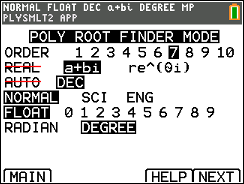
\includegraphics[width=0.31\linewidth]{gc/72_gc1.png}}\hfill\fhl{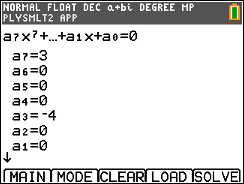
\includegraphics[width=0.31\linewidth]{gc/72_gc2.png}}\hfill\fhl{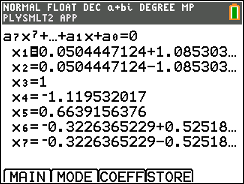
\includegraphics[width=0.31\linewidth]{gc/72_gc3.png}}\par}\end{gtpart}
\begin{gtpart}{(b)}{4}New Series: $br,br^{3},br^{5},\dots$
\begin{topalign}
\left|\frac{br}{1-r^{2}}-S\right|&\geqslant1.78b\\\left|\frac{br}{1-r^{2}}-\frac{b}{1-r}\left(1-r^{n}\right)\right|&\geqslant1.78b\\\left|\frac{0.6639b}{1-0.6639^{2}}-\frac{b}{1-0.6639}\left(1-0.6639^{n}\right)\right|&\geqslant1.78b\\\left|\frac{0.6639}{1-0.6639^{2}}-\frac{1}{1-0.6639}\left(1-0.6639^{n}\right)\right|&\geqslant1.78\quad(\because b>0)
\end{topalign}
Using GC,
\begin{topalign}
&\text{When }n=14,\ \left|\frac{0.6639}{1-0.6639^{2}}-\frac{1}{1-0.6639}\left(1-0.6639^{n}\right)\right|=1.7785<1.78\\&\text{When }n=15,\ \left|\frac{0.6639}{1-0.6639^{2}}-\frac{1}{1-0.6639}\left(1-0.6639^{n}\right)\right|=1.7818\geqslant1.78
\end{topalign}
Therefore, least $n=15$.\end{gtpart}}
%% ============================================================ 73  SAJC 2025 Prelim P1 Q5
\defQ{73}{}{%
An arithmetic progression has first term $a$ and common difference $d$, where $a$ and $d$ are non-zero. The 3rd, 9th and 11th terms of the arithmetic progression are three distinct consecutive terms of a geometric progression.
\begin{qparts}
\pt{(a)} Find $d$ in terms of $a$. \mk{3}
\pt{(b)} Let the sum of the first $n$ terms of the arithmetic progression be $S_n$ where $S_1=143$. Find the largest possible value of $S_n$. \mk{3}
\end{qparts}
The first term of the geometric progression is $b$, where $b$ is positive.
\begin{qparts}
\pt{(c)} Determine whether the geometric series is convergent. \mk{2}
\pt{(d)} Show that the sum of all terms after the $n$th term of the geometric progression is at most $\frac12b$, where $n$ is a positive integer. \mk{2}
\end{qparts}
\src{SAJC 2025 Prelim P1 Q5}}
\defS{73}{%
\begin{gtpart}{(a)}{3}\begin{topalign}
\frac{a+8d}{a+2d}&=\frac{a+10d}{a+8d}\\(a+8d)^{2}&=(a+2d)(a+10d)\\a^{2}+16ad+64d^{2}&=a^{2}+12ad+20d^{2}\\4ad+44d^{2}&=0\\4d(a+11d)&=0
\end{topalign}
$d=0$ (reject since terms of AP, GP are distinct)\quad or\quad $a+11d=0$\par
\hspace*{0.5\linewidth}$d=-\dfrac{1}{11}a$\end{gtpart}
\begin{gtpart}{(b)}{3}\begin{topalign}
S_1=a&=143\\d&=-\frac{1}{11}(143)=-13\\S_n&=\frac{n}{2}\left[2a+(n-1)d\right]\\&=\frac{n}{2}\left[286-13(n-1)\right]
\end{topalign}
From GC, largest $S_n=858$
\par\smallskip{\centering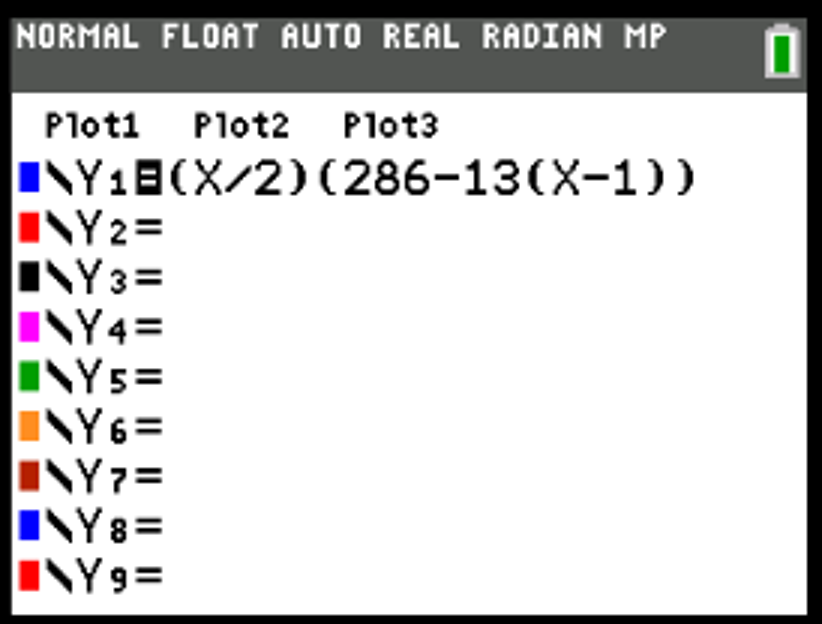
\includegraphics[width=0.48\linewidth]{gc/73_gc1.png}\hfill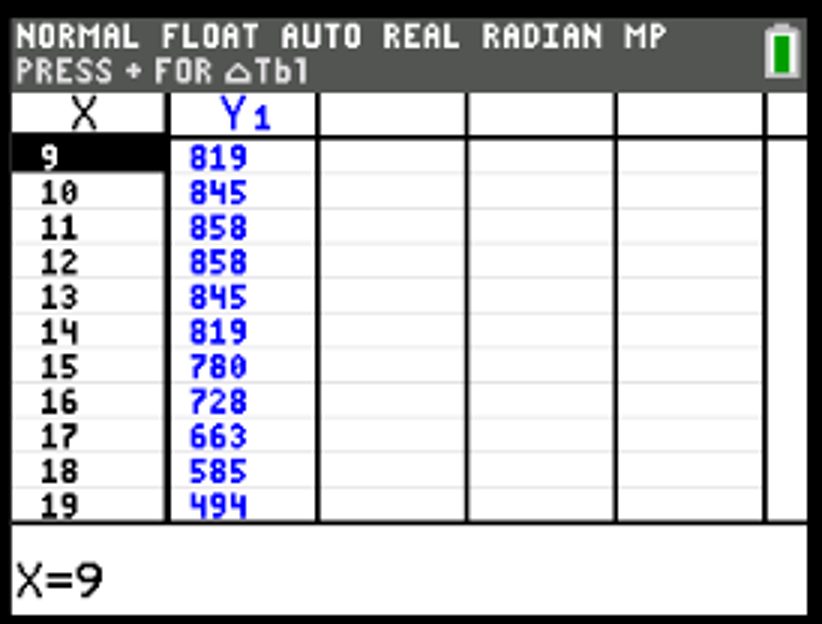
\includegraphics[width=0.48\linewidth]{gc/73_gc2.png}\par}
\end{gtpart}
\begin{gtpart}{(c)}{2}\begin{topalign}
r=\frac{a+8d}{a+2d}=\frac{-11d+8d}{-11d+2d}=\frac{-3d}{-9d}=\frac13
\end{topalign}
Since $|r|=\dfrac13<1$, the geometric series is convergent.\end{gtpart}
\begin{gtpart}{(d)}{2}Let $u_n$ be the $n$th term of the geometric progression.
\begin{topalign}
&u_{n+1}+u_{n+2}+\dots\\&=S_\infty-S_n\\&=\frac{b}{1-r}-\frac{b\left(1-r^{n}\right)}{1-r}\\&=\frac{br^{n}}{1-r}\\&=\frac{b\left(\frac13\right)^{n}}{1-\frac13}\\&=\frac32\left(\frac13\right)^{n}b\\&=\frac{b}{2}\left(\frac13\right)^{n-1}\leqslant\frac12b\quad\text{since }\left(\frac13\right)^{n-1}\leqslant1
\end{topalign}
Alternative:
\begin{topalign}
&u_{n+1}+u_{n+2}+u_{n+3}+\dots\\&=b\left(\frac13\right)^{n}+b\left(\frac13\right)^{n+1}+b\left(\frac13\right)^{n+2}+\dots\\&=\frac{b\left(\frac13\right)^{n}}{1-\frac13}\\&=\frac32b\left(\frac13\right)^{n}\\&=\frac{b}{2}\left(\frac13\right)^{n-1}\leqslant\frac{b}{2}\quad\text{since }\left(\frac13\right)^{n-1}\leqslant1
\end{topalign}\end{gtpart}}
%% ============================================================ 74  TJC 2025 Prelim P1 Q7
\defQ{74}{}{%
Mabel and Janice decided to start a 5-year savings plan beginning in January 2026.\par
Mabel saves using a piggy bank. At the start of January 2026, she deposits \$101. Each subsequent month, she increases her deposit by \$1---so she deposits \$101 in January, \$102 in February, \$103 in March, and so on, until \$112 in December. At the start of each new year, she resets her monthly deposit to \$101 in January and repeats the same pattern through December. She continues this routine from 2026 to 2030, inclusive.\par
Janice, on the other hand, deposits \$100 at the start of every month into a bank account that earns 0.3\% interest per month, with interest calculated and added into the account at the end of each month.
\begin{qparts}
\pt{(a)} Show that Janice will have more money in her savings account than Mabel has in her piggy bank at the end of December 2030. \mk{5}
\pt{(b)} Find the month and year when Janice's savings first exceed Mabel's savings. \mk{4}
\end{qparts}
\src{TJC 2025 Prelim P1 Q7}}
\defS{74}{%
\begin{gtpart}{(a)}{5}For Mabel:\par
Amount of money Mabel saves in a year
\begin{topalign}
&=\$(101+102+\dots+112)\\&=\$\frac{12}{2}(101+112)=\$1278
\end{topalign}
Amount of money Mabel saves in 5 year $=\$1278\times5=\$6390$\par\medskip
For Janice:\par\smallskip
{\small\renewcommand{\arraystretch}{1.3}\begin{tabular}{|l|l|l|}\hline
$n$th mth&Amount at start of month (\$)&Amount at end of month (\$)\\\hline
1 Jan26&$100$&$100(1.003)$\\\hline
2&$\begin{aligned}[t]&100+100(1.003)\\&=100(1+1.003)\end{aligned}$&$\begin{aligned}[t]&100(1+1.003)(1.003)\\&=100\left(1.003+1.003^{2}\right)\end{aligned}$\\\hline
$\vdots$&&$\vdots$\\\hline
$n$&&$\begin{aligned}[t]&100\left(1.003+1.003^{2}+\dots+1.003^{n}\right)\\&=\frac{100(1.003)\left(1.003^{n}-1\right)}{1.003-1}\end{aligned}$\\\hline
\end{tabular}}\par\medskip
At Dec 2030, $n=60$.\par
Therefore, Amount Janice saves in 5 years
\begin{topalign}
=\frac{100(1.003)\left(1.003^{60}-1\right)}{1.003-1}=\$6582.85\ \text{(2 d.p.) [A1]}
\end{topalign}
$\therefore$ Janice will have more money in her savings account than Mabel has in her piggy bank.\end{gtpart}
\begin{gtpart}{(b)}{4}At end of 4\textsuperscript{th} year,\par
Mabel will have \$1278 x 4 $=\$5112$\par
Janice will have $\dfrac{100(1.003)\left(1.003^{48}-1\right)}{1.003-1}=\$5169.97>\$5112$\par\smallskip
At end of 3\textsuperscript{rd} year,\par
Mabel will have \$1278 x 3 $=\$3834$\par
Janice will have $\dfrac{100(1.003)\left(1.003^{36}-1\right)}{1.003-1}=\$3806.97<\$3834$\par\smallskip
Therefore, the year when Janice's saving is more than Mabel's saving happen in 4\textsuperscript{th} year (i.e. 2029). Let it be the $k$\textsuperscript{th} month.\par
Then set Janice's saving $>$ Mabel's saving
\begin{topalign}
&\Rightarrow\frac{100(1.003)\left(1.003^{36+k}-1\right)}{1.003-1}>3834+\frac{k}{2}\left[2(100)+(k-1)(1)\right]\\&\Rightarrow\left(\frac{100003}{3}\right)\left(1.003^{36+k}-1\right)-3834-\frac{k}{2}\left[199+k\right]>0
\end{topalign}
Using GC, we have $k\geqslant4$. Therefore, the month and year is Apr 2029.\end{gtpart}}
%% ============================================================ 75  ACJC 2025 Prelim P1 Q12
\defQ{75}{}{%
Sarah, a Singaporean Citizen, started a 4-year undergraduate Computing course at the National University of Singapore (NUS) in August 2021. The annual tuition fee, after the MOE Tuition Grant, is \$8,250. Sarah took a Tuition Fee Loan (TFL) covering 90\% of her tuition fees. This loan is interest-free during her course of study.\par
Sarah decided to set aside \$$x$ per month from August 2021. This amount is increased by \$2 each subsequent month. (Sarah set aside \$$x$ in August 2021, \$$(x+2)$ in September 2021, \dots.) With the amount set aside, she repaid one-fifth of her total TFL at the end of July 2025.
\begin{qparts}
\pt{(a)} Find the value of $x$. \mk{3}
\end{qparts}
Upon Sarah's graduation, the TFL's interest rate becomes effective at a fixed rate of 0.4\% per month, calculated on the outstanding balance at the end of the month. The interest is first charged on 31st August 2025.\par
Sarah plans to make monthly repayments of \$$y$ to the bank on the 1st of every month, starting from 1st September 2025.
\begin{qparts}
\pt{(b)} Find the amount of outstanding loan after Sarah's first monthly repayment. \mk{1}
\pt{(c)} Show that the amount of outstanding loan after Sarah's $n$th monthly repayment is
\[23760(1.004)^{n}-250y\left(1.004^{n}-1\right).\] \mk{3}
\pt{(d)} Sarah wants to pay off her remaining loan by the end of 3 years. Find the value of $y$. \mk{2}
\end{qparts}
Sarah decided on a different repayment strategy. For the first 24 months, she repays \$500 per month. After these 24 months, she doubles her monthly repayment to \$1000.
\begin{qparts}
\pt{(e)} Determine the month and year Sarah will clear her loan and calculate the amount of her final repayment. \mk{4}
\end{qparts}
\src{ACJC 2025 Prelim P1 Q12}}
\defS{75}{%
\begin{gtpart}{(a)}{3}Amount Sarah plans to repay (before graduation):\par
$\dfrac15\times\dfrac{90}{100}\times8250\times4=\$5940$\par\smallskip
Number of repayments made from August 2021 to July 2025 is 48 (i.e. $n=48$).\par
The repayments follow an arithmetic progression (AP) with first term $a=x$ and common difference $d=2$.\par\smallskip
The sum of an arithmetic progression is
\begin{topalign}
S_n&=\frac{n}{2}\left[2a+(n-1)d\right]\\5940&=\frac{48}{2}\left[2x+(48-1)2\right]\\x&=76.75
\end{topalign}\end{gtpart}
\begin{gtpart}{(b)}{1}Amount of outstanding loan after Sarah's graduation:\par
$\dfrac45\times\dfrac{90}{100}\times8250\times4=\$23760$\par\smallskip
On 31\textsuperscript{st} August 2025, apply interest of 0.4\% to outstanding loan to get $\$\left(23760(1.004)\right)$.\par
On 1\textsuperscript{st} September 2025, make 1\textsuperscript{st} repayment of \$$y$ to the bank.\par\smallskip
$\therefore$ Outstanding loan after 1\textsuperscript{st} repayment\par
$=\$\left(23760(1.004)-y\right)$ or $\$(23855.04-y)$\end{gtpart}
\begin{gtpart}{(c)}{3}On 30\textsuperscript{th} September 2025, apply interest of 0.4\%.\par
On 1\textsuperscript{st} October 2025, make 2\textsuperscript{nd} repayment of \$$y$.\par
Outstanding loan after 2\textsuperscript{nd} repayment
\begin{topalign}
&=\left(23760(1.004)-y\right)1.004-y\\&=23760(1.004)^{2}-1.004y-y
\end{topalign}
Outstanding loan after 3\textsuperscript{rd} repayment (on 1\textsuperscript{st} Nov 2025)
\begin{topalign}
&=\left(23760(1.004)^{2}-1.004y-y\right)1.004-y\\&=23760(1.004)^{3}-1.004^{2}y-1.004y-y
\end{topalign}
Outstanding loan after $n$\textsuperscript{th} repayment
\begin{topalign}
&=23760(1.004)^{n}-1.004^{n-1}y-\dots-1.004^{2}y-1.004y-y\\&=23760(1.004)^{n}-y\left(1+1.004+1.004^{2}+\dots+1.004^{n-1}\right)\\&=23760(1.004)^{n}-y\left(\frac{1.004^{n}-1}{1.004-1}\right)\\&=23760(1.004)^{n}-250y\left(1.004^{n}-1\right)\ \text{(shown)}
\end{topalign}\end{gtpart}
\begin{gtpart}{(d)}{2}To repay remaining loan by the end of 3 years (i.e. 36 monthly repayments of \$$y$), let $n=36$.\par\smallskip
To fully repay the loan, we want outstanding loan amount after 36 repayments to be zero (or less).
\begin{topalign}
23760(1.004)^{36}-250y\left(1.004^{36}-1\right)&\leqslant0\\y&\geqslant709.9769\\\therefore\ y&=709.98\ \text{(nearest cent)}
\end{topalign}\end{gtpart}
\begin{gtpart}{(e)}{4}After 24 monthly repayments of \$500 (i.e. $n=24$, $y=500$), outstanding loan amount
\begin{topalign}
&=23760(1.004)^{24}-250(500)\left((1.004)^{24}-1\right)\\&=13580.49
\end{topalign}
Outstanding loan amount as of 1\textsuperscript{st} August 2027\par
$=13580.49$\par
In a similar method to \textbf{(c)}, the outstanding loan amount after $m$ monthly repayments of \$1000 (i.e. $y=1000$) is\par
$13580.49(1.004)^{m}-250(1000)\left((1.004)^{m}-1\right)$\par\smallskip
To fully repay the loan, we need
\begin{topalign}
13580.49(1.004)^{m}-250(1000)\left((1.004)^{m}-1\right)&\leqslant0\\m&\geqslant13.991185\\\text{Least }m&=14
\end{topalign}
Sarah would require another 14 monthly repayments to fully repay her loan, with her first repayment of \$1000 on 1\textsuperscript{st} September 2027.\par\smallskip
Hence, she would clear her loan on \underline{(1st) October 2028}.\par\smallskip
The outstanding loan amount after her 13\textsuperscript{th} monthly repayment of \$1000 (on 1\textsuperscript{st} Sep 2028) is
\begin{topalign}
&13580.49(1.004)^{13}-250(1000)\left((1.004)^{13}-1\right)\\&=987.2529
\end{topalign}
Interest is applied on 30\textsuperscript{th} Sep 2028. Hence her final repayment amount is\par
$987.2529\times1.004=\underline{\$991.20}$ (nearest cent)\par\smallskip
(Alternatively, outstanding loan amount after 14\textsuperscript{th} monthly repayment is
\begin{topalign}
&13580.49(1.004)^{14}-250(1000)\left((1.004)^{14}-1\right)\\&=-8.7981
\end{topalign}
Hence the final repayment is $1000-8.7981=\$991.20$ (nearest cent).\end{gtpart}}
%% ============================================================ 76  RVHS 2025 Prelim P2 Q4
\defQ{76}{}{%
The dosage of medicine given to a patient needs to be carefully managed in order to achieve the desired result.
\begin{qparts}
\pt{(a)} To give the patient time to adapt to a particular medicine, the dosage is slowly increased over time. The patient is initially given a dosage of 0.75 units. The dosage is increased by 0.5 units each day until a total of at least 10 units of medicine has been taken. Find the least number of days it takes to achieve this, and the dosage on that day. \mk{4}
\pt{(b)} The doctor prescribed a new medication to another patient. After $n$ days, the total dosage of the new medicine administered to the patient is given by
\[\frac{3}{20}\left(\frac{5^{n}-4^{n}}{5^{n-1}}\right)\ \text{units.}\]
\begin{qparts}
\pt{(i)} Show that the increase in dosage of the new medicine administered per day follows a geometric progression. \mk{3}
\pt{(ii)} Find the total dosage of the new medicine administered to the patient after a long period of treatment. \mk{2}
\end{qparts}
\pt{(c)} Doctors can manage the medication so that the daily dosage of medicine increases as an arithmetic progression. Explain in context why the arithmetic progression is not a preferred model for the dosage of medication. \mk{1}
\end{qparts}
\src{RVHS 2025 Prelim P2 Q4}}
\defS{76}{%
\begin{gtpart}{(a)}{4}Let $u_n$ be the dose on the $n^{th}$ day.
\begin{topalign}
u_n&=0.75+0.5(n-1)\\S_n&=\frac{n}{2}\left(2(0.75)+(n-1)(0.5)\right)\\10&\leqslant\frac{n}{2}\left(1+\frac{n}{2}\right)\qquad\text{-----}(*)\\\frac14n^{2}+\frac12n&\geqslant10\\n^{2}+2n&\geqslant40\\(n+1)^{2}&\geqslant41\\n\geqslant-1+\sqrt{41}\ &\text{or}\ n\leqslant-1-\sqrt{41}\\&\text{(rej as no. of days cannot be -ve)}\\n&\geqslant5.40312
\end{topalign}
Therefore, it takes 6 days.\par\smallskip
Alternatively,\par
When $n=5$, $\frac14n^{2}+\frac12n=8.75<10$\par
When $n=6$, $\frac14n^{2}+\frac12n=12\geqslant10$\par
Therefore, it takes 6 days.\par\smallskip
$u_6=0.75+0.5(5)=3.25$\par
The dose on the 6\textsuperscript{th} day is 3.25 units.\end{gtpart}
\begin{gtpart}{(b)(i)}{3}Increase on $n^{th}$ day
\begin{topalign}
&=S_n-S_{n-1}\\&=\frac{3}{20}\left(\frac{5^{n}-4^{n}}{5^{n-1}}\right)-\frac{3}{20}\left(\frac{5^{n-1}-4^{n-1}}{5^{n-2}}\right)\\&=\frac{3}{20}\left(\frac{5^{n}-4^{n}}{5^{n-1}}-\frac{5^{n-1}-4^{n-1}}{5^{n-2}}\right)\\&=\frac{3}{20}\left(\frac{1}{5^{n-2}}\right)\left(5^{n-1}-\frac45\left(4^{n-1}\right)-5^{n-1}+4^{n-1}\right)\\&=\frac{3}{20}\left(\frac{1}{5^{n-2}}\right)\left(\frac15\right)\left(4^{n-1}\right)\\&=\frac{3}{20}\left(\frac45\right)^{n-1}
\end{topalign}
which is of the form $ar^{n-1}$, where $a=\dfrac{3}{20}$ and $r=\dfrac45$ which is a GP.\par\smallskip
\textbf{\underline{Alternative:}}\par
Consider $\dfrac{u_{n+1}}{u_n}=\dfrac{\frac{3}{20}\left(\frac45\right)^{n+1-1}}{\frac{3}{20}\left(\frac45\right)^{n-1}}=\dfrac45$ which is a constant\par\smallskip
Since consecutive terms have a common ratio $r=\dfrac45$, the increase in dosage follows a GP.\end{gtpart}
\begin{gtpart}{(b)(ii)}{2}\textbf{\underline{Method 1}}\par
Long term dosage
\begin{topalign}
&=\lim_{n\to\infty}\frac{3}{20}\left(\frac{5^{n}-4^{n}}{5^{n-1}}\right)\\&=\frac{3/20}{1-4/5}\\&=\frac34
\end{topalign}
In the long term, the total dosage approaches 0.75 units.\par\smallskip
\textbf{Note:}\par
After $n$ days, the total dosage of the medicine is given by $\dfrac{3}{20}\left(\dfrac{5^{n}-4^{n}}{5^{n-1}}\right)$.\par
Let $S_n$ denote the total dosage of the new medicine after $n$ days.\par
Then $S_n=\dfrac{3}{20}\left(\dfrac{5^{n}-4^{n}}{5^{n-1}}\right)$.\par
Let $v_n$ the change in dosage on $n$th day found in part (b)(i) where $v_n=S_n-S_{n-1}$\par
Since $v_n$ is a geometric progression, we can use $S_\infty=\dfrac{a}{1-r}$, the sum to infinity formula to find the long term total dosage.\par\smallskip
\textbf{\underline{Method 2}}
\begin{topalign}
&\frac{3}{20}\left(\frac{5^{n}-4^{n}}{5^{n-1}}\right)\\&=\frac{3}{20}(5)\left(\frac{5^{n}-4^{n}}{5^{n}}\right)\\&=\frac{3}{20}(5)\left(1-\left(\frac45\right)^{n}\right)
\end{topalign}
As $n\to\infty$, $\left(\dfrac45\right)^{n}\to0$\par
Total dosage in the long term
\begin{topalign}
&=\frac{3}{20}(5)(1-0)\\&=\frac34
\end{topalign}\end{gtpart}
\begin{gtpart}{(c)}{1}If the dosage increases as an AP, then it will continue to \textbf{\underline{increase to}} (positive) \textbf{\underline{infinity}}.\end{gtpart}}
%% ============================================================ 81  RVHS 2025 Prelim P1 Q7(a)
\defQ{81}{}{%
A curve $C$ has equation $x^{2}+y^{2}-4y=xy$, where $x\geqslant0$.
\begin{qparts}
\pt{(a)} Show that $\left(2y-x-4\right)\dfrac{\mathrm{d}y}{\mathrm{d}x}=y-2x$. \mk{2}
\end{qparts}
\src{RVHS 2025 Prelim P1 Q7(a)}}
\defS{81}{%
\begin{gtpart}{(a)}{2}\begin{topalign}
x^{2}+y^{2}-4y&=xy\\2x+2y\frac{\mathrm{d}y}{\mathrm{d}x}-4\frac{\mathrm{d}y}{\mathrm{d}x}&=y+x\frac{\mathrm{d}y}{\mathrm{d}x}\\\left(2y-x-4\right)\frac{\mathrm{d}y}{\mathrm{d}x}+2x-y&=0\\\left(2y-x-4\right)\frac{\mathrm{d}y}{\mathrm{d}x}&=y-2x
\end{topalign}\end{gtpart}}
%% ============================================================ 82  (no source; written to Maximus's request)
\defQ{82}{}{%
A curve has parametric equations $x=t+\sin t$, $y=1-\cos t$.
\begin{qparts}
\pt{} Show that $\dfrac{\mathrm{d}y}{\mathrm{d}x}=\tan\dfrac{t}{2}$. \mk{3}
\end{qparts}}
\defS{82}{%
\begin{gtpart}{}{3}\begin{topalign}
x=t+\sin t\ &\Rightarrow\ \frac{\mathrm{d}x}{\mathrm{d}t}=1+\cos t\\
y=1-\cos t\ &\Rightarrow\ \frac{\mathrm{d}y}{\mathrm{d}t}=\sin t\\
\frac{\mathrm{d}t}{\mathrm{d}x}&=\frac{1}{\frac{\mathrm{d}x}{\mathrm{d}t}}=\frac{1}{1+\cos t}\\
\frac{\mathrm{d}y}{\mathrm{d}x}&=\frac{\mathrm{d}y}{\mathrm{d}t}\times\frac{\mathrm{d}t}{\mathrm{d}x}\\
&=\frac{\sin t}{1+\cos t}\\
&=\frac{2\sin\frac{t}{2}\cos\frac{t}{2}}{2\cos^{2}\frac{t}{2}}\\
&=\frac{\sin\frac{t}{2}}{\cos\frac{t}{2}}\\
&=\tan\frac{t}{2}\quad\text{(shown)}
\end{topalign}\end{gtpart}}
% Ch9 rates / max-min diagrams, redrawn in TikZ from the original papers
\usetikzlibrary{calc,arrows.meta,angles,quotes}
\tikzset{c9/.style={line width=0.7pt},c9d/.style={dashed,line width=0.5pt},c9a/.style={-{Stealth[length=2mm]},line width=0.5pt},c9aa/.style={{Stealth[length=2mm]}-{Stealth[length=2mm]},line width=0.5pt}}
\newcommand{\rtmark}[3]{\draw[line width=0.4pt] ($(#1)!#3!(#2)$) -- ($($(#1)!#3!(#2)$)!#3!90:(#2)$) -- ($(#1)!#3!90:(#2)$);}
% TJC 2025 P2 Q4: Figures 1 and 2
\newcommand{\figTJCfa}{\begin{tikzpicture}[scale=1]
\coordinate (O) at (0,0); \coordinate (A) at (230:1.8); \coordinate (B) at (310:1.8);
\draw[c9] (A) -- (O) -- (B) arc[start angle=310,end angle=590,radius=1.8];
\draw[line width=0.5pt] (310:0.22) arc[start angle=310,end angle=590,radius=0.22];
\node at (0,0.55) {$\theta$}; \node[below=1pt] at (O) {$O$};
\node at ($(O)!0.55!(A)+(-0.18,0.12)$) {$a$}; \node at ($(O)!0.55!(B)+(0.18,0.12)$) {$a$};
\node[below left] at (A) {$A$}; \node[below right] at (B) {$B$};
\node at (0,-2.2) {Figure 1};
\end{tikzpicture}}
\newcommand{\figTJCfb}{\begin{tikzpicture}[scale=1]
\draw[c9] (0,0) ellipse (1.3 and 0.25); \draw[c9] (-1.3,0) -- (0,1.7) -- (1.3,0);
\draw[c9d] (0,1.7) -- (0,0) -- (1.3,0); \draw[line width=0.4pt] (0,0.15)--(0.15,0.15)--(0.15,0);
\node[above right] at (0.7,0.85) {$a$}; \node[below] at (0.75,0) {$r$};
\node at (0,-1.6) {Figure 2};
\end{tikzpicture}}
% TJC 2025 P2 Q4: Figure 3 (two cones tip-to-tip)
\newcommand{\figTJCfc}{\begin{tikzpicture}[scale=1]
\draw[c9] (0,1.6) ellipse (1.15 and 0.22); \draw[c9] (0,-1.6) ellipse (1.15 and 0.22);
\draw[c9] (-1.15,1.6) -- (1.15,-1.6); \draw[c9] (1.15,1.6) -- (-1.15,-1.6);
\draw[c9d] (0,1.6) -- (0,-1.6); \draw[c9d] (0,1.6) -- (-1.15,1.6); \draw[c9d] (0,-1.6) -- (1.15,-1.6);
\draw[line width=0.4pt] (0,1.45)--(0.15,1.45)--(0.15,1.6); \draw[line width=0.4pt] (0,-1.45)--(0.15,-1.45)--(0.15,-1.6);
\node[above] at (-0.6,1.6) {$r$}; \node[below] at (0.6,-1.6) {$r$};
\node[left] at (-0.65,0.85) {$a$}; \node[right] at (0.65,-0.85) {$a$};
\node at (0,-2.4) {Figure 3};
\end{tikzpicture}}
% DHS 2025 P1 Q11: tank
\newcommand{\figDHSa}{\begin{tikzpicture}[scale=1]
\draw[c9] (0,2.6) ellipse (1 and 0.28);
\draw[c9] (-1,2.6) -- (-1,0); \draw[c9] (1,2.6) -- (1,0);
\draw[c9d] (1,0) arc[start angle=0,end angle=180,x radius=1,y radius=0.28];
\draw[c9d] (-1,0) arc[start angle=180,end angle=360,x radius=1,y radius=0.28];
\draw[c9] (-1,0) arc[start angle=180,end angle=360,radius=1];
\draw[c9aa] (-1.3,2.45) -- (-1.3,0); \node[left] at (-1.3,1.25) {$L$};
\draw[c9a] (0,0) -- (0.95,0); \node[above] at (0.45,0) {$r$};
\end{tikzpicture}}
% DHS 2025 P1 Q11: hemispherical bottom with water
\newcommand{\figDHSb}{\begin{tikzpicture}[scale=1.1,blue!60!black]
\fill[blue!12] (-1.47,-1.05) arc[start angle=215.7,end angle=324.3,radius=1.8] -- cycle;
\draw[c9,black!70!blue] (-1.8,0) -- (1.8,0); \draw[c9,black!70!blue] (-1.8,0) arc[start angle=180,end angle=360,radius=1.8];
\node[black,above] at (-0.9,0) {15}; \node[black,above] at (0.9,0) {15};
\draw[c9d,thick] (0,0) -- (0,-1.05); \draw[c9d] (0,0) -- (-1.47,-1.05);
\draw[line width=0.6pt] (-1.47,-1.05) -- (1.47,-1.05);
\draw[c9a,thick] (0,-1.05) -- (-1.45,-1.05); \node[black,above] at (-0.7,-1.05) {$x$};
\draw[c9aa,thick] (0,-1.05) -- (0,-1.8); \node[black,right] at (0,-1.45) {$h$};
\end{tikzpicture}}
% DHS solution (c)(i) diagram
\newcommand{\figDHSsol}{\begin{tikzpicture}[scale=1]
\draw[line width=0.5pt] (-1.8,0) -- (1.8,0); \draw[line width=0.5pt] (-1.8,0) arc[start angle=180,end angle=360,radius=1.8];
\node[above] at (-0.9,0.05) {\small 15}; \node[above] at (0.9,0.05) {\small 15};
\draw[line width=0.5pt] (0,0) -- (-1.47,-1.05) -- (0,-1.05) -- cycle; \draw[line width=0.4pt] (0,-0.9)--(-0.15,-0.9)--(-0.15,-1.05);
\draw[line width=0.5pt] (-1.47,-1.05) -- (1.47,-1.05);
\node[above] at (-0.9,-0.5) {\small 15}; \node[right] at (0,-0.5) {\small $15-h$}; \node[below] at (-0.75,-1.05) {\small $x$};
\draw[c9aa] (0.3,-1.05) -- (0.3,-1.8); \node[right] at (0.3,-1.45) {\small $h$};
\end{tikzpicture}}
% TJC 2024 Promo Q12: sphere inscribed in inverted cone
\newcommand{\figTJCsph}[1][0]{\begin{tikzpicture}[scale=1]
\coordinate (A) at (0,-3); \coordinate (C) at (-1.6,0); \coordinate (B) at (1.6,0); \coordinate (O) at (0,0); \coordinate (P) at (0,-0.96);
\coordinate (D) at ($(C)!(P)!(A)$);
\draw[c9] (O) ellipse (1.6 and 0.45); \draw[c9] (C) -- (A) -- (B); \draw[c9] (P) circle (0.96);
\draw[c9d] (C) -- (O); \draw[c9d] (O) -- (A); \draw[c9d] (P) -- (D);
\rtmark{O}{C}{0.13} \rtmark{D}{P}{0.11}
\node[above,font=\small,inner sep=1pt] at (-0.8,0.02) {$r$ cm}; \node[above right,inner sep=1pt] at (0.05,0.02) {$O$};
\node[above,font=\small,inner sep=1pt] at ($(P)!0.55!(D)+(0.05,0.05)$) {$R$ cm};
\ifnum#1=0 \draw[c9aa,dotted] (2.1,0.1) -- (2.1,-3); \node[right] at (2.1,-1.45) {$h$ cm};
\else \node[left] at (C) {$C$}; \node[right] at (B) {$B$}; \node[below left] at (D) {$D$}; \node[below] at (A) {$A$}; \node[right] at (P) {$P$}; \node[right] at (0.1,-0.6) {$h$ cm};\fi
\end{tikzpicture}}
% CJC 2024 Promo Q10: paper cone cup
\newcommand{\figCJC}{\begin{tikzpicture}[scale=1]
\fill[gray!55] (-1.25,0) -- (0,-2.9) -- (1.25,0) arc[start angle=0,end angle=-180,x radius=1.25,y radius=0.25];
\draw[c9,fill=white] (0,0) ellipse (1.25 and 0.25); \draw[c9] (-1.25,0) -- (0,-2.9) -- (1.25,0);
\draw[c9d] (0,0) -- (0,-2.9); \draw[line width=0.4pt] (0,0.13)--(0.13,0.13)--(0.13,0);
\draw[c9a] (0.05,0) -- (1.22,0); \node[above] at (0.65,0.02) {$r$};
\draw[line width=0.4pt,dotted] (-1.8,0) -- (-1.25,0); \draw[line width=0.4pt,dotted] (-1.8,-2.9) -- (0,-2.9);
\draw[c9aa,line width=0.6pt] (-1.75,0) -- (-1.75,-2.9); \node[left] at (-1.75,-1.45) {$h$};
\end{tikzpicture}}
% CJC solution (d) diagram
\newcommand{\figCJCsol}{\begin{tikzpicture}[scale=0.9,blue!70!black]
\draw[line width=0.7pt] (0,0) ellipse (1.1 and 0.25); \draw[line width=0.7pt] (-1.1,0) -- (0,-2.4) -- (1.1,0);
\draw[c9a] (0,-2.4) -- (0,0); \draw[c9a] (0,0) -- (1.05,0); \node[above] at (0.55,0) {$r$}; \node[left] at (0,-1) {$h$};
\draw[c9a] (0,-1.1) -- (0.55,-1.1); \node[above] at (0.3,-1.1) {$x$};
\draw[c9aa] (1.4,-1.1) -- (1.4,-2.4); \node[right] at (1.4,-1.75) {$y$};
\end{tikzpicture}}
% EJC 2018 Promo Q7: right cone, slant edge R
\newcommand{\figEJC}{\begin{tikzpicture}[scale=1]
\draw[c9] (0,0) ellipse (1.7 and 0.18); \draw[c9] (-1.7,0) -- (0,3) -- (1.7,0);
\draw[c9d] (0,3) -- (0,0); \draw[c9aa] (0,0) -- (1.68,0); \node[below] at (0.85,0) {$x$};
\draw[c9aa] ($(-1.7,0)+(-0.2,-0.1)$) -- ($(0,3)+(-0.2,-0.1)$); \node[left] at (-1.05,1.6) {$R$}; \node[right] at (0,1.6) {$h$};
\end{tikzpicture}}
% TMJC 2024 Prelim P1 Q2: cylinder inscribed in sphere
\newcommand{\figTMJC}{\begin{tikzpicture}[scale=1]
\draw[c9] (0,0) circle (1.75);
\draw[c9] (0,0.85) ellipse (1.53 and 0.25); \draw[c9] (-1.53,0.85) -- (-1.53,-0.85); \draw[c9] (1.53,0.85) -- (1.53,-0.85);
\draw[c9] (-1.53,-0.85) arc[start angle=180,end angle=360,x radius=1.53,y radius=0.25];
\draw[c9d] (1.53,-0.85) arc[start angle=0,end angle=180,x radius=1.53,y radius=0.25];
\draw[c9aa,dashed] (0,-0.85) -- (0,0.85); \node[left] at (0,0.45) {$h$};
\fill (0,0) circle (1.6pt); \draw[c9d] (0,0) -- (1.53,-0.85); \node[above right] at (0.75,-0.4) {$k$};
\draw[c9d] (0,-0.85) -- (1.53,-0.85); \node[above] at (0.7,-0.88) {\small$r$};
\end{tikzpicture}}
% TMJC solution triangle
\newcommand{\figTMJCsol}{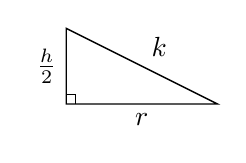
\begin{tikzpicture}[scale=0.8]
\draw[line width=0.5pt] (0,0) -- (2.4,0) -- (0,1.2) -- cycle; \draw[line width=0.4pt] (0,0.15)--(0.15,0.15)--(0.15,0);
\node[left] at (0,0.6) {$\frac{h}{2}$}; \node[below] at (1.2,0) {$r$}; \node[above right] at (1.2,0.6) {$k$};
\end{tikzpicture}}
% RVHS 2025 Promo Q1 solution diagram (conical tank with water)
\newcommand{\figRVHSsol}{\begin{tikzpicture}[scale=0.85]
\fill[blue!15] (-0.9,-1.5) -- (0,-3) -- (0.9,-1.5) arc[start angle=0,end angle=-180,x radius=0.9,y radius=0.15];
\draw[blue!50,fill=blue!8] (0,-1.5) ellipse (0.9 and 0.15);
\draw[c9] (0,0) ellipse (1.8 and 0.3); \draw[c9] (-1.8,0) -- (0,-3) -- (1.8,0);
\draw[c9aa] (0,0) -- (1.78,0); \node[above] at (0.9,0) {$3$};
\draw[c9aa] (-0.15,0) -- (-0.15,-3); \node[left] at (-0.15,-0.8) {$6$};
\draw[c9a] (0,-1.5) -- (0.88,-1.5); \node[above] at (0.45,-1.5) {$r$};
\draw[c9aa] (0.15,-1.5) -- (0.15,-3); \node[right] at (0.15,-2.2) {$h$};
\end{tikzpicture}}
\newcommand{\dD}{\mathrm{d}}
\providecommand{\solnotfound}{\par\noindent\fbox{\parbox{0.9\linewidth}{\centering\color{red}\textbf{Official solution not found}}}\par}
%% ============================================================ 91  RVHS 2025 Promo Q1  (soln: promo25/promo_rv_sa.pdf p15)
\defQ{91}{}{%
A conical water tank is being filled with water at a constant rate of $0.2\ \text{m}^{3}\text{s}^{-1}$. The tank has a height of 6 m and a radius at the top of 3 m.
\begin{qparts}
\pt{(a)} Show that the volume of the water in the tank, $V$, can be expressed as $\dfrac{2}{3}\pi r^{3}$, where $r$ is the radius of the top water surface. \mk{1}
\pt{(b)} Find the exact rate of change of $r$ when the height of the water is 4 m. \mk{3}
\end{qparts}
[The volume of a cone of base radius $r$ and height $h$ is given by $V=\dfrac{1}{3}\pi r^{2}h$.]
\src{RVHS 2025 Promo Q1}}
\defS{91}{%
\begin{gtpart}{(a)}{1}{\centering\figRVHSsol\par}
\begin{topalign}
V&=\frac{1}{3}\pi r^{2}h,\ \text{where $h$ is the height of the water.}\\
&=\frac{1}{3}\pi r^{2}(2r),\ \text{since }\frac{h}{r}=\frac{6}{3}=\frac{2}{1}\text{ by similar triangles.}\\
&=\frac{2}{3}\pi r^{3}.\ \text{(Shown)}
\end{topalign}\end{gtpart}
\begin{gtpart}{(b)}{3}\begin{topalign}
\frac{\dD V}{\dD r}&=2\pi r^{2}
\end{topalign}
When $h=4$ (i.e. when $r=2$),
\begin{topalign}
\frac{\dD r}{\dD t}&=\frac{\dD r}{\dD V}\times\frac{\dD V}{\dD t}\\
&=\frac{1}{2\pi r^{2}}\times0.2\\
&=\frac{1}{8\pi}\times0.2\\
&=\frac{1}{40\pi}\ \text{m s}^{-1}
\end{topalign}\end{gtpart}}
%% ============================================================ 92  TJC 2025 Prelim P2 Q4  (soln: TJC_2025_H2_Math_Prelim_P2_Solutions.pdf pp4-6)
\defQ{92}{}{%
[The arc length $L$ of a sector of radius $a$ and angle $\theta$ is given by $L=a\theta$;\par
The volume $V$ of a cone of base radius $r$ and height $h$ is given by $V=\dfrac{1}{3}\pi r^{2}h$\,]
\begin{center}\figTJCfa\hspace{1.5cm}\raisebox{0.6cm}{\figTJCfb}\end{center}
A metal sheet is shaped as a circular sector with angle $\theta$ and fixed radius $a$, as shown in Figure 1. This sector is then formed into a right circular cone with slant height $a$ by joining the two radii $OA$ and $OB$ together as shown in Figure 2.
\begin{qparts}
\pt{(a)} If $\theta$ is measured in radians, state the base radius of the cone, $r$, in term of $a$ and $\theta$. \mk{1}
\pt{(b)} Show that the volume of the cone, $V$, is given by
\[V^{2}=\frac{a^{6}}{576\pi^{4}}\theta^{4}\left(4\pi^{2}-\theta^{2}\right).\] \mk{3}
\pt{(c)} Using differentiation, find the exact value of $\theta$ that will maximise $V$. \mk{4}
\end{qparts}
\begin{center}\figTJCfc\end{center}
Two identical cones, as described in part \textbf{(c)}, are joined together tip-to-tip to form a new object, as shown in Figure 3. The upper cone is initially filled with water, which leaks out into the lower cone at a rate of $\dfrac{\pi}{15}\ \text{cm}^{3}\,\text{s}^{-1}$. At time $t$ seconds, the height of the water in the upper cone is $y$.
\begin{qparts}
\pt{(d)} Show that the volume of water in the cone, $W$ cm$^{3}$, is given by $W=\dfrac{2\pi y^{3}}{3}$. \mk{2}
\pt{(e)} Calculate the rate of change of $y$ when $y=2$. \mk{2}
\end{qparts}
\src{TJC 2025 Prelim P2 Q4}}
\defS{92}{%
\begin{gtpart}{(a)}{1}Circumference of base = length of arc AB
\begin{topalign}
2\pi r&=a\theta\\
r&=\frac{a}{2\pi}\theta
\end{topalign}\end{gtpart}
\begin{gtpart}{(b)}{3}(i)\quad Let $h$ = height of cone
\begin{topalign}
h^{2}&=a^{2}-r^{2}\\
&=a^{2}-\frac{a^{2}}{4\pi^{2}}\theta^{2}\\
&=\frac{a^{2}}{4\pi^{2}}\left(4\pi^{2}-\theta^{2}\right)\\
V&=\frac{1}{3}\pi r^{2}h\\
V^{2}&=\frac{1}{9}\pi^{2}r^{4}h^{2}\\
&=\frac{1}{9}\pi^{2}\left(\frac{a^{4}}{16\pi^{4}}\right)\cdot\frac{a^{2}}{4\pi^{2}}\left(4\pi^{2}-\theta^{2}\right)\\
&=\frac{a^{6}}{576\pi^{4}}\theta^{4}\left(4\pi^{2}-\theta^{2}\right)
\end{topalign}\end{gtpart}
\begin{gtpart}{(c)}{4}\textbf{Method 1}
\begin{topalign}
\frac{\dD V^{2}}{\dD\theta}&=\frac{a^{6}}{576\pi^{4}}\frac{\dD}{\dD\theta}\left(4\pi^{2}\theta^{4}-\theta^{6}\right)\\
&=\frac{a^{6}}{576\pi^{4}}\left(16\pi^{2}\theta^{3}-6\theta^{5}\right)\\
&=\frac{a^{6}}{576\pi^{4}}\cdot2\theta^{3}\left(8\pi^{2}-3\theta^{2}\right)\\
\frac{\dD V^{2}}{\dD\theta}&=0\ \text{when }\theta^{3}\left(8\pi^{2}-3\theta^{2}\right)=0\\
\theta^{2}&=\frac{8\pi^{2}}{3}\quad\Rightarrow\ \theta=2\pi\sqrt{\frac{2}{3}}\\
\frac{\dD^{2}V^{2}}{\dD\theta^{2}}&=\frac{a^{6}}{576\pi^{4}}\left(48\pi^{2}\theta^{2}-30\theta^{4}\right)
\end{topalign}
When $\theta=2\pi\sqrt{\dfrac{2}{3}}$,
\begin{topalign}
\frac{\dD^{2}V^{2}}{\dD\theta^{2}}&=\frac{a^{6}}{576\pi^{4}}\left(48\pi^{2}\left(\frac{8\pi^{2}}{3}\right)-30\left(\frac{64\pi^{4}}{9}\right)\right)=-\frac{4a^{6}}{27}<0
\end{topalign}
Therefore $V$ is max when $\theta=2\pi\sqrt{\dfrac{2}{3}}$\par\medskip
\textbf{Method 2}
\begin{topalign}
V^{2}&=\frac{a^{6}}{576\pi^{4}}\theta^{4}\left(4\pi^{2}-\theta^{2}\right)
\end{topalign}
Differentiating w.r.t. $\theta$,
\begin{topalign}
2V\frac{\dD V}{\dD\theta}&=\frac{a^{6}}{576\pi^{4}}\frac{\dD}{\dD\theta}\left(4\pi^{2}\theta^{4}-\theta^{6}\right)\\
&=\frac{a^{6}}{576\pi^{4}}\left(16\pi^{2}\theta^{3}-6\theta^{5}\right)\\
&=\frac{a^{6}}{576\pi^{4}}\cdot2\theta^{3}\left(8\pi^{2}-3\theta^{2}\right)\\
\frac{\dD V}{\dD\theta}&=0\ \text{when }\theta^{3}\left(8\pi^{2}-3\theta^{2}\right)=0\\
\theta^{2}&=\frac{8\pi^{2}}{3}\quad\Rightarrow\ \theta=2\pi\sqrt{\frac{2}{3}}\quad(\because\theta>0)\\
2V\frac{\dD^{2}V}{\dD\theta^{2}}+2\left(\frac{\dD V}{\dD\theta}\right)^{2}&=\frac{a^{6}}{576\pi^{4}}\left(48\pi^{2}\theta^{2}-30\theta^{4}\right)
\end{topalign}
When $\theta=2\pi\sqrt{\dfrac{2}{3}}$, $\dfrac{\dD V}{\dD\theta}=0$
\begin{topalign}
2V\frac{\dD^{2}V}{\dD\theta^{2}}&=\frac{a^{6}}{576\pi^{4}}\left(48\pi^{2}\left(\frac{8\pi^{2}}{3}\right)-30\left(\frac{64\pi^{4}}{9}\right)\right)=-\frac{4a^{6}}{27}<0
\end{topalign}
Since $V>0$, $\dfrac{\dD^{2}V}{\dD\theta^{2}}<0$\par
Therefore $V$ is max when $\theta=2\pi\sqrt{\dfrac{2}{3}}$\end{gtpart}
\begin{gtpart}{(d)}{2}Note that: $\theta=2\pi\sqrt{\dfrac{2}{3}}$
\begin{topalign}
r&=\frac{a}{2\pi}\theta=\frac{a}{2\pi}\left(2\pi\sqrt{\frac{2}{3}}\right)=a\sqrt{\frac{2}{3}}\\
h^{2}&=a^{2}-r^{2}=a^{2}-\left(a\sqrt{\frac{2}{3}}\right)^{2}=\frac{1}{3}a^{2}\quad\Rightarrow\ h=\frac{1}{\sqrt{3}}a\\
\frac{r}{h}&=a\sqrt{\frac{2}{3}}\times\frac{\sqrt{3}}{a}=\sqrt{2}\quad\Rightarrow\ r=\sqrt{2}h\\
W&=\frac{1}{3}\pi r_{w}^{2}h_{w}=\frac{1}{3}\pi\left(\sqrt{2}y\right)^{2}y=\frac{2\pi y^{3}}{3}
\end{topalign}\end{gtpart}
\begin{gtpart}{(e)}{2}\begin{topalign}
\frac{\dD W}{\dD t}&=\frac{\dD W}{\dD y}\times\frac{\dD y}{\dD t}\\
-\frac{\pi}{15}&=2\pi y^{2}\times\frac{\dD y}{\dD t}\\
\frac{\dD y}{\dD t}&=-\frac{1}{30y^{2}}
\end{topalign}
When $y=2$, $\dfrac{\dD y}{\dD t}=-\dfrac{1}{120}$ cm s$^{-1}$\par
Rate of change of $y$ is $-\dfrac{1}{120}$ cm s$^{-1}$.\end{gtpart}}
%% ============================================================ 93  DHS 2025 Prelim P1 Q11  (soln: DHS_2025_H2_Math_Prelim_P1_Solutions.pdf pp20-22)
\defQ{93}{}{%
[The surface area and volume of a sphere are given by $4\pi r^{2}$ and $\dfrac{4}{3}\pi r^{3}$ respectively.]\par\medskip
An aquarist who has a fixed budget of \$$k$ wants to make a goldfish sanctuary. His design of the tank consists of a circular cover, a cylinder of length $L$ cm and a hemispherical base of radius $r$ cm neatly fitted together. The costs of the material per cm$^{2}$ used for the cover, the cylindrical surface and hemispherical base are \$20, \$10 and \$30 respectively. Assume that the tank is made of material with negligible thickness.
\begin{center}\figDHSa\end{center}
\begin{qparts}
\pt{(a)} Show that the volume of the tank is $V$ cm$^{3}$, where $V=\dfrac{k}{20}r-\dfrac{10}{3}\pi r^{3}$. \mk{3}
\pt{(b)} As $r$ varies, find the cost of the material used to make the hemispherical base in terms of $k$ when $V$ is at its maximum value. You need to show that $V$ is a maximum. \mk{3}
\end{qparts}
The aquarist has fixed the radius of the cylinder to be 15 cm. Initially, there is some water in the hemispherical part of the tank. However, due to a defect in the tank, water is leaking at a constant rate of 20 cm$^{3}$ per minute.\par\smallskip
The depth of the water at the hemispherical bottom is denoted by $h$ cm, and the radius of the water surface is $x$ cm. The volume of water in the hemispherical bottom is given by $W$ cm$^{3}$, where $W=\dfrac{\pi h\left(3x^{2}+h^{2}\right)}{6}$.
\begin{center}\figDHSb\end{center}
\begin{qparts}
\pt{(c)} By formulating a relationship between $x$ and $h$, find, when $h=3$, the rate of change of
\begin{qparts}
\pt{(i)} the depth of water, \mk{3}
\pt{(ii)} the radius of the water surface. \mk{3}
\end{qparts}
\end{qparts}
\src{DHS 2025 Prelim P1 Q11}}
\defS{93}{%
\begin{gtpart}{(a)}{3}\begin{topalign}
k&=2\pi r^{2}(30)+2\pi rL(10)+\pi r^{2}(20)\\
k&=80\pi r^{2}+20\pi rL\\
k&=20\pi r(4r+L)\\
\Rightarrow L&=\frac{k}{20\pi r}-4r\\
V&=\frac{2}{3}\pi r^{3}+\pi r^{2}L\\
&=\frac{2}{3}\pi r^{3}+\pi r^{2}\left(\frac{k}{20\pi r}-4r\right)\\
&=\frac{2}{3}\pi r^{3}+\frac{kr}{20}-4\pi r^{3}\\
&=\frac{k}{20}r-\frac{10}{3}\pi r^{3}\ \text{(shown)}
\end{topalign}\end{gtpart}
\begin{gtpart}{(b)}{3}For maximum $V$ as $r$ varies,
\begin{topalign}
\frac{\dD V}{\dD r}&=0\\
\frac{\dD V}{\dD r}&=\frac{k}{20}-10\pi r^{2}\\
r&=\sqrt{\frac{k}{200\pi}}\quad\text{(reject $r<0$)}\\
\frac{\dD^{2}V}{\dD r^{2}}&=-20\pi r<0
\end{topalign}
Therefore, $V$ is maximum.\par\smallskip
Cost of material for the hemispherical base
\begin{topalign}
&=2\pi r^{2}(30)=2\pi\left(\sqrt{\frac{k}{200\pi}}\right)^{2}(30)=\frac{3k}{10}\ \text{dollars}
\end{topalign}\end{gtpart}
\begin{gtpart}{(c)(i)}{3}{\centering\figDHSsol\par}
By Pythagoras' Theorem,
\begin{topalign}
x^{2}&=15^{2}-(15-h)^{2}\\
x^{2}&=\left(15-(15-h)\right)\left(15+(15-h)\right)\\
x^{2}&=h(30-h)\\
W&=\frac{\pi h\left(3x^{2}+h^{2}\right)}{6}=\frac{\pi h\left(3\left(h(30-h)\right)+h^{2}\right)}{6}\\
W&=\frac{\pi h\left(90h-2h^{2}\right)}{6}=\frac{\pi\left(45h^{2}-h^{3}\right)}{3}\\
\frac{\dD W}{\dD h}&=\frac{\pi\left(90h-3h^{2}\right)}{3}\\
\frac{\dD W}{\dD t}&=\frac{\dD W}{\dD h}\times\frac{\dD h}{\dD t}=\frac{\pi\left(90h-3h^{2}\right)}{3}\times\frac{\dD h}{\dD t}
\end{topalign}
At $h=3$,
\begin{topalign}
\frac{\dD h}{\dD t}&=\frac{\frac{\dD W}{\dD t}}{\frac{\dD W}{\dD h}}=\frac{-20}{\frac{\pi\left(90(3)-3(3)^{2}\right)}{3}}\\
&=-0.078595=-0.0786\ \text{cm/min}\ \text{(3 s.f.)}
\end{topalign}\end{gtpart}
\begin{gtpart}{(c)(ii)}{3}\begin{topalign}
\frac{\dD x}{\dD t}&=\frac{\dD x}{\dD h}\times\frac{\dD h}{\dD t}\\
x^{2}&=h(30-h)\Rightarrow x=\sqrt{h(30-h)}=\sqrt{30h-h^{2}}\quad(x>0)\\
\frac{\dD x}{\dD h}&=\frac{30-2h}{2\sqrt{30h-h^{2}}}=\frac{15-h}{\sqrt{30h-h^{2}}}
\end{topalign}
At $h=3$,
\begin{topalign}
\frac{\dD x}{\dD t}&=\left(\frac{15-3}{\sqrt{30(3)-(3)^{2}}}\right)\times(-0.078595)\\
&=-0.10479=-0.105\ \text{cm/min}\ \text{(3sf)}
\end{topalign}\end{gtpart}}
%% ============================================================ 94  TJC 2024 Promo Q12 (soln: TJC Promo 2024.pdf pp26-28)
\defQ{94}{}{%
[It is given that the volume of cone with radius $r$ and height $h$ is $\dfrac{1}{3}\pi r^{2}h$\,]\par\medskip
A water filter system takes the shape of an inverted right circular cone with a circular top of radius $r$ cm and height $h$ cm. It contains a spherical filter which the water passes through during filtration. The sphere has a constant radius $R$ cm and is inscribed in the cone such that the sphere is in contact with the center of the circular top, $O$, and the slant surface of the cone as shown in the diagram below.
\begin{center}\figTJCsph\end{center}
\begin{qparts}
\pt{(a)} Show that $r^{2}=\dfrac{h^{2}R^{2}}{h^{2}-2hR}$. \mk{3}
\pt{(b)} As $h$ varies, find the minimum volume of the cone in terms of $R$. \mk{5}\par
[You do not need to show that the volume is minimum]
\end{qparts}
\src{TJC 2024 Promo Q12}}
\defS{94}{%
\begin{gtpart}{(a)}{3}{\centering\figTJCsph[1]\par}
Let centre of the sphere be $P$.\par
Using similar triangles $APD$ and $ACO$,
\begin{topalign}
\frac{h-R}{AC}&=\frac{R}{r}\\
AC&=\frac{rh-rR}{R}
\end{topalign}
By Pythagoras' Theorem, $AC^{2}=h^{2}+r^{2}$
\begin{topalign}
\left(\frac{rh-rR}{R}\right)^{2}&=h^{2}+r^{2}\\
r^{2}h^{2}-2r^{2}hR+r^{2}R^{2}&=h^{2}R^{2}+r^{2}R^{2}\\
r^{2}\left(h^{2}-2hR\right)&=h^{2}R^{2}\\
\therefore\ r^{2}&=\frac{h^{2}R^{2}}{h^{2}-2hR}
\end{topalign}
\textbf{OR}\par
Let centre of the sphere be $P$.
\begin{topalign}
AD&=\sqrt{\left(AP^{2}-PD^{2}\right)}\\
&=\sqrt{\left((h-R)^{2}-R^{2}\right)}\\
&=\sqrt{\left(h^{2}-2hR\right)}
\end{topalign}
Using congruent triangles $PCO$ and $PCD$, $CO=CD=r$ cm.
\begin{topalign}
AC&=AD+DC\\
&=\sqrt{\left(h^{2}-2hR\right)}+r
\end{topalign}
Since by Pythagoras' theorem, $AC^{2}=h^{2}+r^{2}$
\begin{topalign}
h^{2}+r^{2}&=h^{2}-2hR+2r\sqrt{\left(h^{2}-2hR\right)}+r^{2}\\
\therefore\ r^{2}&=\frac{h^{2}R^{2}}{h^{2}-2hR}
\end{topalign}\end{gtpart}
\begin{gtpart}{(b)}{5}Volume of cone, $V$
\begin{topalign}
&=\tfrac{1}{3}\pi r^{2}h\\
&=\tfrac{1}{3}\pi\frac{h^{2}R^{2}}{h^{2}-2hR}h\\
&=\tfrac{1}{3}\pi R^{2}\frac{h^{3}}{h^{2}-2hR}\\
&=\tfrac{1}{3}\pi R^{2}\frac{h^{2}}{h-2R}\\
\frac{\dD V}{\dD h}&=\tfrac{1}{3}\pi R^{2}\left[\frac{2h(h-2R)-h^{2}}{(h-2R)^{2}}\right]\\
&=\tfrac{1}{3}\pi R^{2}\left[\frac{h^{2}-4hR}{(h-2R)^{2}}\right]\\
&=\tfrac{1}{3}\pi R^{2}\frac{h(h-4R)}{(h-2R)^{2}}\\
\frac{\dD V}{\dD h}&=0\\
\tfrac{1}{3}\pi R^{2}\frac{h(h-4R)}{(h-2R)^{2}}&=0\\
h&=4R\ \text{or}\ h=0\ (\text{reject}\ \because h>0)\\
\therefore\ \text{minimum }V&=\tfrac{1}{3}\pi R^{2}\frac{(4R)^{2}}{4R-2R}=\tfrac{8}{3}\pi R^{3}\ \text{cm}^{3}
\end{topalign}\end{gtpart}}
%% ============================================================ 95  CJC 2024 Promo Q10 (soln: CJC Promo 2024.pdf pp21-24)
\defQ{95}{}{%
\mbox{}\par\vspace{-1ex}\begin{center}\figCJC\end{center}
A cone-shaped cup is made of paper of negligible thickness to hold $20\pi$ cm$^{3}$ of liquid. The open inverted cone has radius $r$ cm and height $h$ cm as shown in the diagram above.\par
The external surface area of the cup is denoted by $A$ cm$^{2}$. The manufacturer wants to reduce the cost of production by minimizing the value of $A$.
\begin{qparts}
\pt{(a)} Find $h$ in terms of $r$. \mk{1}
\pt{(b)} By considering $A^{2}$ or otherwise, show that $A\dfrac{\dD A}{\dD r}=\pi^{2}\left(2r^{3}-\dfrac{3600}{r^{3}}\right)$. \mk{3}
\pt{(c)} Find the exact value of $r$ that gives the minimum value of $A$, proving that $A$ is a minimum. Find also the ratio of the radius to the height, $\dfrac{r}{h}$, giving your answer in terms of $k\sqrt{2}$, where $k$ is a constant to be determined. \mk{5}
\end{qparts}
The manufacturer decides to make paper cups at minimum external surface area using the ratio $\dfrac{r}{h}$ found in part \textbf{(c)}.
\begin{qparts}
\pt{(d)} The cup is being filled completely with water. However, there is a small hole at the bottom of the cup that causes water to leak out at the rate of 3 cm$^{3}$ per second. Find the rate of decrease of the depth of the water at the instant when the depth is 2 cm. \mk{3}
\end{qparts}
[It is given that the volume of a circular cone with base radius $r$ and height $h$ is $\dfrac{1}{3}\pi r^{2}h$ and the curved surface area is $\pi rl$, where $l$ is the slant height of the cone.]
\src{CJC 2024 Promo Q10}}
\defS{95}{%
\begin{gtpart}{(a)}{1}\begin{topalign}
\text{Volume of cone}&=\frac{1}{3}\pi r^{2}h=20\pi\\
\frac{r^{2}h}{3}&=20\\
h&=\frac{60}{r^{2}}
\end{topalign}\end{gtpart}
\begin{gtpart}{(b)}{3}\underline{\textbf{Method 1: Considering $A^{2}$}}
\begin{topalign}
A&=\pi rl\\
&=\pi r\sqrt{r^{2}+h^{2}}\\
&=\pi r\sqrt{r^{2}+\left(\frac{60}{r^{2}}\right)^{2}}\\
&=\pi r\sqrt{r^{2}+\frac{3600}{r^{4}}}\\
A^{2}&=\pi^{2}r^{2}\left(r^{2}+\frac{3600}{r^{4}}\right)\\
&=\pi^{2}\left(r^{4}+\frac{3600}{r^{2}}\right)\\
&=\pi^{2}\left(r^{4}+3600r^{-2}\right)
\end{topalign}
Differentiating implicitly with respect to $r$:
\begin{topalign}
2A\frac{\dD A}{\dD r}&=\pi^{2}\left(4r^{3}-7200r^{-3}\right)\\
A\frac{\dD A}{\dD r}&=\pi^{2}\left(2r^{3}-\frac{3600}{r^{3}}\right)\quad\text{(shown)}
\end{topalign}
\underline{\textbf{Method 2: ``Otherwise'' Method}}
\begin{topalign}
A&=\pi rl\\
&=\pi r\sqrt{r^{2}+h^{2}}\\
&=\pi r\sqrt{r^{2}+\left(\frac{60}{r^{2}}\right)^{2}}\\
&=\pi r\sqrt{r^{2}+\frac{3600}{r^{4}}}\\
&=\pi r\left(r^{2}+3600r^{-4}\right)^{\frac{1}{2}}
\end{topalign}
Differentiating with respect to $r$:
\begin{topalign}
\frac{\dD A}{\dD r}&=\pi\left[r\cdot\frac{1}{2}\left(r^{2}+3600r^{-4}\right)^{-\frac{1}{2}}\left(2r-4\cdot3600r^{-5}\right)+\left(r^{2}+3600r^{-4}\right)^{\frac{1}{2}}\right]\\
&=\pi\left(r^{2}+3600r^{-4}\right)^{-\frac{1}{2}}\left[r^{2}-7200r^{-4}+r^{2}+3600r^{-4}\right]\\
&=\pi\left(r^{2}+3600r^{-4}\right)^{-\frac{1}{2}}\left[2r^{2}-3600r^{-4}\right]\\
&=\frac{\pi}{\sqrt{r^{2}+3600r^{-4}}}\left(2r^{2}-\frac{3600}{r^{4}}\right)\\
A\frac{\dD A}{\dD r}&=\pi r\sqrt{r^{2}+3600r^{-4}}\cdot\frac{\pi}{\sqrt{r^{2}+3600r^{-4}}}\left(2r^{2}-\frac{3600}{r^{4}}\right)\\
&=\pi^{2}r\left(2r^{2}-\frac{3600}{r^{4}}\right)\\
&=\pi^{2}\left(2r^{3}-\frac{3600}{r^{3}}\right)\quad\text{(shown)}
\end{topalign}\end{gtpart}
\begin{gtpart}{(c)}{5}At stationary point, $\dfrac{\dD A}{\dD r}=0$
\begin{topalign}
\pi^{2}\left(2r^{3}-\frac{3600}{r^{3}}\right)&=0\\
2r^{3}-\frac{3600}{r^{3}}&=0\\
2r^{3}&=\frac{3600}{r^{3}}\\
r^{6}&=1800\\
r&=(1800)^{\frac{1}{6}}
\end{topalign}
To prove minimum:\par
\underline{\textbf{Method 1: Using 1\textsuperscript{st} derivative test}}\par\smallskip
{\renewcommand{\arraystretch}{1.6}\begin{tabular}{|c|c|c|c|}\hline
$r$&$\left((1800)^{\frac{1}{6}}\right)^{-}$&$(1800)^{\frac{1}{6}}$&$\left((1800)^{\frac{1}{6}}\right)^{+}$\\\hline
Sign of $\dfrac{\dD A}{\dD r}$&$<0$&$0$&$>0$\\\hline
Tangent&\tikz\draw[blue](0,0.25)--(0.4,0);&\tikz\draw[blue](0,0)--(0.4,0);&\tikz\draw[blue](0,0)--(0.4,0.25);\\\hline
\end{tabular}}\par\smallskip
$r=(1800)^{\frac{1}{6}}$ gives the minimum $A$.\par\medskip
\underline{\textbf{Method 2: Using 2\textsuperscript{nd} derivative test}}\par
From the result $A\dfrac{\dD A}{\dD r}=\pi^{2}\left(2r^{3}-\dfrac{3600}{r^{3}}\right)$, using implicit differentiation to obtain:
\begin{topalign}
A\frac{\dD^{2}A}{\dD r^{2}}+\left(\frac{\dD A}{\dD r}\right)^{2}&=\pi^{2}\left(6r^{2}+\frac{10800}{r^{4}}\right)
\end{topalign}
At $\dfrac{\dD A}{\dD r}=0$ and $r=(1800)^{\frac{1}{6}}$, $\dfrac{\dD^{2}A}{\dD r^{2}}=\dfrac{\pi^{2}}{A}\left(6r^{2}+\dfrac{10800}{r^{4}}\right)>0$ (minimum)\par
$r=(1800)^{\frac{1}{6}}$ gives the minimum $A$.\par\medskip
\underline{\textbf{Method 3:}}
\begin{topalign}
\frac{r}{h}&=\frac{r}{\left(\frac{60}{r^{2}}\right)}\\
&=\frac{r^{3}}{60}\\
&=\frac{\left(1800^{\frac{1}{6}}\right)^{3}}{60}\\
&=\frac{\sqrt{1800}}{60}\\
&=\frac{30\sqrt{2}}{60}\\
&=\frac{\sqrt{2}}{2},\ \text{where }k=\frac{1}{2}
\end{topalign}
\underline{\textbf{Method 4:}}
\begin{topalign}
h&=\frac{60}{r^{2}}\\
&=\frac{60}{\left(1800^{\frac{1}{6}}\right)^{2}}\\
&=\frac{60}{1800^{\frac{1}{3}}}\\
\frac{r}{h}&=\frac{1800^{\frac{1}{6}}}{\left(\frac{60}{1800^{\frac{1}{3}}}\right)}\\
&=\frac{\sqrt{1800}}{60}\\
&=\frac{30\sqrt{2}}{60}\\
&=\frac{\sqrt{2}}{2},\ \text{where }k=\frac{1}{2}
\end{topalign}\end{gtpart}
\begin{gtpart}{(d)}{3}Let $V$ be the volume of water in the cone when radius of water surface is $x$ cm and depth is $y$ cm.\par
By similar triangles,\par
{\centering\figCJCsol\par}
\begin{topalign}
\frac{x}{y}&=\frac{r}{h}=\frac{\sqrt{2}}{2}\\
x&=\frac{\sqrt{2}}{2}y\\
V&=\frac{1}{3}\pi x^{2}y\\
&=\frac{1}{3}\pi\left(\frac{\sqrt{2}}{2}y\right)^{2}y\\
&=\frac{1}{6}\pi y^{3}\\
\frac{\dD V}{\dD y}&=\frac{1}{2}\pi y^{2}\\
\frac{\dD V}{\dD t}&=\frac{\dD V}{\dD y}\times\frac{\dD y}{\dD t}\\
&=\frac{1}{2}\pi y^{2}\times\frac{\dD y}{\dD t}
\end{topalign}
When $y=2$,
\begin{topalign}
-3&=\frac{1}{2}\pi(2)^{2}\times\frac{\dD y}{\dD t}\\
\frac{\dD y}{\dD t}&=-\frac{3}{2\pi}
\end{topalign}
Rate of decrease of depth of water is $\dfrac{3}{2\pi}$ cm/s or 0.477 cm/s (3 s.f.)\end{gtpart}}
%% ============================================================ 96  EJC 2018 Promo Q7 (soln: Promo2018.pdf pp107-109)
\defQ{96}{}{%
\mbox{}\par\vspace{-1ex}\begin{center}\figEJC\end{center}
The diagram shows a right cone with a slant edge of fixed length $R$ cm, height $h$ cm and radius $x$ cm.\par\smallskip
Show that $9V^{2}=\pi^{2}x^{4}\left(R^{2}-x^{2}\right)$, where $V$ is the volume of the cone.\par\smallskip
\begin{qparts}
\pt{} Show further that, as $x$ varies, $V$ is a maximum when $x^{2}=\dfrac{2}{3}R^{2}$. \mk{7}
\end{qparts}
\src{EJC 2018 Promo Q7}}
\defS{96}{%
\begin{gtpart}{}{7}\begin{topalign}
h&=\sqrt{R^{2}-x^{2}}\\
V&=\frac{1}{3}\pi x^{2}h\\
&=\frac{1}{3}\pi x^{2}\sqrt{R^{2}-x^{2}}\\
V^{2}&=\frac{1}{9}\pi^{2}x^{4}\left(\sqrt{R^{2}-x^{2}}\right)^{2}\\
9V^{2}&=\pi^{2}x^{4}\left(R^{2}-x^{2}\right)\ \text{(shown)}
\end{topalign}
Differentiate w.r.t. $x$,
\begin{topalign}
9V^{2}&=\pi^{2}R^{2}x^{4}-\pi^{2}x^{6}\\
18V\frac{\dD V}{\dD x}&=4\pi^{2}R^{2}x^{3}-6\pi^{2}x^{5}\ \text{--- (*)}
\end{topalign}
When the volume is maximum, $\dfrac{\dD V}{\dD x}=0$
\begin{topalign}
-6\pi^{2}x^{5}+4\pi^{2}R^{2}x^{3}&=0\\
2\pi^{2}x^{3}\left(-3x^{2}+2R^{2}\right)&=0\\
-3x^{2}+2R^{2}&=0\ \text{or}\ x=0\ (\text{reject}\ \because x>0)\\
x^{2}&=\frac{2}{3}R^{2}\Rightarrow R^{2}=\frac{3}{2}x^{2}
\end{topalign}
\textbf{Check that $V$ is indeed a maximum:}\par
\underline{Second derivative method}\par
Differentiating (*) wrt $x$
\begin{topalign}
18V\frac{\dD^{2}V}{\dD x^{2}}+18\left(\frac{\dD V}{\dD x}\right)^{2}&=12\pi^{2}R^{2}x^{2}-30\pi^{2}x^{4}
\end{topalign}
Substitute $x^{2}=\dfrac{2}{3}R^{2}$, $\dfrac{\dD V}{\dD x}=0$,
\begin{topalign}
18V\frac{\dD^{2}V}{\dD x^{2}}+18(0)^{2}&=12\pi^{2}R^{2}\left(\frac{2R^{2}}{3}\right)-30\pi^{2}\left(\frac{2R^{2}}{3}\right)^{2}\\
18V\frac{\dD^{2}V}{\dD x^{2}}&=\frac{-40}{3}\pi^{2}R^{4}+8\pi^{2}R^{4}\\
18V\frac{\dD^{2}V}{\dD x^{2}}&=-\frac{16}{3}\pi^{2}R^{4}\\
\frac{\dD^{2}V}{\dD x^{2}}&=-\frac{16\pi^{2}R^{4}}{54V}<0
\end{topalign}
Therefore, $V$ is a maximum when $x^{2}=\dfrac{2}{3}R^{2}$.\par\medskip
\underline{First derivative method}\par
From (*),
\begin{topalign}
\frac{\dD V}{\dD x}&=\frac{4\pi^{2}R^{2}x^{3}-6\pi^{2}x^{5}}{18V}=\frac{\pi^{2}x^{3}\left(2R^{2}-3x^{2}\right)}{9V}
\end{topalign}
(\textit{Note to students}: Since $\dfrac{\pi^{2}x^{3}}{9V}>0$ for all $x$, we just need to consider $\left(2R^{2}-3x^{2}\right)$.)\par\smallskip
{\small\renewcommand{\arraystretch}{1.6}\begin{tabular}{|c|c|c|c|}\hline
$x$&$\left(\sqrt{\frac{2}{3}}R\right)^{-}$&$\sqrt{\frac{2}{3}}R$&$\left(\sqrt{\frac{2}{3}}R\right)^{+}$\\\hline
$\dfrac{\dD V}{\dD x}$&$\begin{aligned}[t]&2R^{2}-3\left[\left(\sqrt{\tfrac{2}{3}}R\right)^{-}\right]^{2}\\&=2R^{2}-\left(2R^{2}\right)^{-}>0\end{aligned}$&$0$&$\begin{aligned}[t]&2R^{2}-3\left[\left(\sqrt{\tfrac{2}{3}}R\right)^{+}\right]^{2}\\&=2R^{2}-\left(2R^{2}\right)^{+}<0\end{aligned}$\\\hline
Slope&/&--&$\backslash$\\\hline
\end{tabular}}\par\smallskip
Therefore, $V$ is a maximum when $x^{2}=\dfrac{2}{3}R^{2}$.\end{gtpart}}
%% ============================================================ 97  TMJC 2024 Prelim P1 Q2 (soln: TMJC_2024_Prelim.pdf pp51-52)
\defQ{97}{}{%
\mbox{}\par\vspace{-1ex}\begin{center}\figTMJC\end{center}
\begin{qparts}
\pt{} A cylinder with height $h$ cm and base radius $r$ cm is inscribed within a sphere with fixed radius $k$ cm. The circumference of the circular top and bottom of the cylinder is in contact with the sphere (see figure above). By using differentiation, find, in terms of $k$, the exact value of $h$ for which the volume of the cylinder is maximum. \mk{6}
\end{qparts}
\src{TMJC 2024 Prelim P1 Q2}}
\defS{97}{%
\begin{gtpart}{}{6}Let $V$ be the volume of the cylinder (in cm$^{3}$).\par
By Pythagoras Theorem,\hfill\figTMJCsol\hspace*{1cm}\null
\begin{topalign}
\left(\frac{h}{2}\right)^{2}+r^{2}&=k^{2}\\
r^{2}&=k^{2}-\frac{h^{2}}{4}\quad\text{--- (1)}\\
V&=\pi r^{2}h\\
&=\pi\left(k^{2}-\frac{h^{2}}{4}\right)h\quad\text{,from (1)}\\
&=\pi k^{2}h-\frac{\pi}{4}h^{3}
\end{topalign}
Differentiate w.r.t $h$,
\begin{topalign}
\frac{\dD V}{\dD h}&=\pi k^{2}-\frac{3\pi}{4}h^{2}
\end{topalign}
For maximum $V$, $\dfrac{\dD V}{\dD h}=0$
\begin{topalign}
\therefore\ \frac{\dD V}{\dD h}&=\pi k^{2}-\frac{3\pi}{4}h^{2}=0\\
k^{2}-\frac{3}{4}h^{2}&=0\\
h^{2}&=\frac{4k^{2}}{3}\\
h&=\frac{2k}{\sqrt{3}}\quad(\because h>0)
\end{topalign}
\underline{\textbf{Testing $V$ is maximum}}\par
\underline{\textbf{Method 1:}} 1\textsuperscript{st} derivative test\par\smallskip
{\renewcommand{\arraystretch}{1.7}\begin{tabular}{|c|c|c|c|}\hline
$h$&$\left(\dfrac{2k}{\sqrt{3}}\right)^{-}$&$\dfrac{2k}{\sqrt{3}}$&$\left(\dfrac{2k}{\sqrt{3}}\right)^{+}$\\\hline
$\dfrac{\dD V}{\dD h}$&$+$&$0$&$-$\\\hline
Slope&\tikz\draw(0,0)--(0.6,0.2);&\tikz\draw(0,0)--(0.6,0);&\tikz\draw(0,0.2)--(0.6,0);\\\hline
\end{tabular}}\par\smallskip
$\therefore V$ is maximum when $h=\dfrac{2k}{\sqrt{3}}$.\par\medskip
\underline{\textbf{Method 2:}} 2\textsuperscript{nd} derivative test\par
Differentiate w.r.t $h$,
\begin{topalign}
\frac{\dD^{2}V}{\dD h^{2}}&=-\frac{3\pi}{2}h
\end{topalign}
When $h=\dfrac{2k}{\sqrt{3}}$, $\dfrac{\dD^{2}V}{\dD h^{2}}=-\dfrac{3\pi}{2}\left(\dfrac{2k}{\sqrt{3}}\right)=-\sqrt{3}\pi k<0\quad(\because k>0)$\par
$\therefore V$ is maximum when $h=\dfrac{2k}{\sqrt{3}}$.\end{gtpart}}
%% ============================================================ 98  EJC 2025 Prelim P2 Q1 (soln: EJC_2025_H2_Math_Prelim_P2_Solutions.pdf p1)
\defQ{98}{}{%
The curve $C$ has equation $x^{3}+y^{3}-3xy=k$, where $k$ is a positive constant.\par
$C$ intersects the $x$-axis at the point $A$.
\begin{qparts}
\pt{(a)} Find the equation of the tangent to $C$ at $A$. Give your answer in the form $y=px+q$, where $p$ and $q$ are constants to be found in terms of $k$. \mk{5}
\pt{(b)} There are two points on $C$ where the tangents are parallel to the $y$-axis. Given that $k=3$, find the exact $y$-coordinates of these two points. \mk{3}
\end{qparts}
\src{EJC 2025 Prelim P2 Q1}}
\defS{98}{%
\begin{gtpart}{(a)}{5}Differentiating $C$ w.r.t. $x$,
\begin{topalign}
3x^{2}+3y^{2}\frac{\dD y}{\dD x}-3x\frac{\dD y}{\dD x}-3y&=0\\
\frac{\dD y}{\dD x}&=\frac{3y-3x^{2}}{3y^{2}-3x}=\frac{y-x^{2}}{y^{2}-x}
\end{topalign}
When $y=0$,
\begin{topalign}
x^{3}&=k,\\
x&=k^{\frac{1}{3}}\\
\frac{\dD y}{\dD x}&=x=k^{\frac{1}{3}}\\
y&=k^{\frac{1}{3}}\left(x-k^{\frac{1}{3}}\right)=k^{\frac{1}{3}}x-k^{\frac{2}{3}}
\end{topalign}\end{gtpart}
\begin{gtpart}{(b)}{3}For tangent to be parallel to $y$-axis, $\dfrac{\dD y}{\dD x}$ must be undefined.\par
Hence,
\begin{topalign}
y^{2}-x&=0\\
x&=y^{2}
\end{topalign}
Substituting into $C$ and $k=3$,
\begin{topalign}
y^{6}+y^{3}-3y^{3}-k&=0\\
y^{6}-2y^{3}-3&=0
\end{topalign}
Factorising,
\begin{topalign}
\left(y^{3}-3\right)\left(y^{3}+1\right)&=0\\
y^{3}=3\quad&\text{or}\quad y^{3}=-1\\
y=3^{\frac{1}{3}}\quad&\text{or}\quad y=-1
\end{topalign}\end{gtpart}}
%% ============================================================ 99  MI 2025 Prelim P2 Q2(i),(ii) (soln: MI_2025_H2_Math_Prelim_P2_Solutions.pdf p2)
\defQ{99}{}{%
A curve $C$ has parametric equations $x=\sqrt{t}$, $y=t^{2}+4$, where $0\leqslant t\leqslant16$.
\begin{qparts}
\pt{(i)} Find the equation of the tangent to $C$ at the point $P$ with parameter $p$. \mk{3}
\pt{(ii)} Given that the tangent in part \textbf{(i)} passes through the point $(0,1)$, find the exact coordinates of the point $P$. \mk{3}
\end{qparts}
\src{MI 2025 Prelim P2 Q2(i), (ii)}}
\defS{99}{%
\begin{gtpart}{(i)}{3}\begin{topalign}
x&=\sqrt{t},\quad y=t^{2}+4\\
\frac{\dD x}{\dD t}&=\frac{1}{2\sqrt{t}},\quad\frac{\dD y}{\dD t}=2t\\
\frac{\dD y}{\dD x}&=\frac{2t}{\frac{1}{2\sqrt{t}}}=4t^{\frac{3}{2}}
\end{topalign}
Note: $t=p$\par
The eqn of tangent to $C$ at $P\left(\sqrt{p},\,p^{2}+4\right)$:
\begin{topalign}
y-\left(p^{2}+4\right)&=4p^{\frac{3}{2}}\left(x-\sqrt{p}\right)\\
y&=4p^{\frac{3}{2}}x-3p^{2}+4
\end{topalign}\end{gtpart}
\begin{gtpart}{(ii)}{3}The eqn of tangent of $C$ at $P$ passes through $(0,1)$\par
At $(0,1)$:
\begin{topalign}
1&=4p^{\frac{3}{2}}(0)-3p^{2}+4\\
3p^{2}&=3\\
p&=1\quad(\text{reject }-1\ \because p\geqslant0)
\end{topalign}
When $p=1$
\begin{topalign}
x&=1,\ y=5\\
&P(1,5)
\end{topalign}\end{gtpart}}
\providecommand{\dD}{\mathrm{d}}
\newcommand{\figEJCtri}{\begin{tikzpicture}[scale=1]
\coordinate (A) at (0,0); \coordinate (C) at (6.6,0.08); \coordinate (B) at (6.6,2.7); \coordinate (X) at (6.6,1.6);
\draw[line width=0.6pt] (A) -- (B) -- (C) -- cycle; \draw[dashed,line width=0.5pt] (A) -- (X);
\draw[line width=0.4pt] ($(C)+(-0.18,0)$) -- ($(C)+(-0.18,0.18)$) -- ($(C)+(0,0.18)$);
\pic[draw,line width=0.4pt,angle radius=1.5cm,"$\alpha$",angle eccentricity=1.2] {angle=X--A--B};
\node[below left] at (A) {$A$}; \node[above] at (B) {$B$}; \node[below right] at (C) {$C$}; \node[right] at (X) {$X$};
\end{tikzpicture}}
%% ============================================================ 101 TJC 2025 Prelim P2 Q1 (soln: TJC_2025_H2_Math_Prelim_P2_Solutions.pdf p1)
\defQ{101}{}{%
It is given that $y=\ln\sqrt{1+\mathrm{e}^{3x}}$.
\begin{qparts}
\pt{(a)} Show that $2\mathrm{e}^{2y}\dfrac{\dD y}{\dD x}=3\mathrm{e}^{3x}$. \mk{2}
\pt{(b)} By further differentiation of the result in part \textbf{(a)}, find the Maclaurin series for $y$, up to and including the term in $x^{2}$, giving the coefficients in exact form. \mk{4}
\pt{(c)} Deduce the Maclaurin series for $\ln\left(\dfrac{\sqrt{1+\mathrm{e}^{-3x}}}{2}\right)$, up to and including the term in $x^{2}$. \mk{2}
\end{qparts}
\src{TJC 2025 Prelim P2 Q1}}
\defS{101}{%
\begin{gtpart}{(a)}{2}\begin{topalign}
y&=\frac{1}{2}\ln\left(1+\mathrm{e}^{3x}\right)\\
\mathrm{e}^{2y}&=1+\mathrm{e}^{3x}
\end{topalign}
Diff. wrt $x$,
\begin{topalign}
2\mathrm{e}^{2y}\frac{\dD y}{\dD x}&=3\mathrm{e}^{3x}\quad\text{(Shown)}\quad\text{-- (1)}
\end{topalign}
\underline{Alternative solution:}
\begin{topalign}
y&=\ln\sqrt{1+\mathrm{e}^{3x}}\\
\frac{\dD y}{\dD x}&=\frac{3\mathrm{e}^{3x}\left(1+\mathrm{e}^{3x}\right)^{-\frac{1}{2}}}{2\left(1+\mathrm{e}^{3x}\right)^{\frac{1}{2}}}=\frac{3\mathrm{e}^{3x}}{2\left(1+\mathrm{e}^{3x}\right)}\\
2\left(1+\mathrm{e}^{3x}\right)\frac{\dD y}{\dD x}&=3\mathrm{e}^{3x}\\
2\mathrm{e}^{2y}\frac{\dD y}{\dD x}&=3\mathrm{e}^{3x}
\end{topalign}
$\left(\because y=\ln\sqrt{1+\mathrm{e}^{3x}}=\dfrac{1}{2}\ln\left(1+\mathrm{e}^{3x}\right)\text{ i.e. }2y=\ln\left(1+\mathrm{e}^{3x}\right)\Rightarrow\mathrm{e}^{2y}=1+\mathrm{e}^{3x}\right)$\end{gtpart}
\begin{gtpart}{(b)}{4}Diff. wrt $x$,
\begin{topalign}
2\mathrm{e}^{2y}\frac{\dD^{2}y}{\dD x^{2}}+4\mathrm{e}^{2y}\left(\frac{\dD y}{\dD x}\right)^{2}&=9\mathrm{e}^{3x}\quad\text{---- (2)}
\end{topalign}
When $x=0$, $y=\dfrac{1}{2}\ln(1+1)=\dfrac{1}{2}\ln2$, $\mathrm{e}^{2y}=\mathrm{e}^{\ln2}=2$
\begin{topalign}
\text{Sub into (1): }\frac{\dD y}{\dD x}&=\frac{3}{4}\\
\text{Sub into (2): }2(2)\frac{\dD^{2}y}{\dD x^{2}}+8\left(\frac{3}{4}\right)^{2}&=9\ \Rightarrow\ \frac{\dD^{2}y}{\dD x^{2}}=\frac{9}{8}\\
y&=\frac{1}{2}\ln2+\frac{3}{4}x+\frac{9}{16}x^{2}+\dots
\end{topalign}\end{gtpart}
\begin{gtpart}{(c)}{2}\begin{topalign}
\ln\left(\frac{\sqrt{1+\mathrm{e}^{-3x}}}{2}\right)&=\ln\left(\sqrt{1+\mathrm{e}^{3(-x)}}\right)-\ln2\\
&=-\ln2+\frac{1}{2}\ln2+\frac{3}{4}(-x)+\frac{9}{16}(-x)^{2}+\dots\\
&=-\frac{1}{2}\ln2-\frac{3}{4}x+\frac{9}{16}x^{2}+\dots
\end{topalign}\end{gtpart}}
%% ============================================================ 102 YIJC 2026 Prelim P1 Q10 (soln: YIJC_2026_P1_Solutions.pdf pp15-17)
\defQ{102}{}{%
It is given that $y=\mathrm{e}^{\sin^{-1}(3x)}$, where $-\dfrac{1}{3}<x<\dfrac{1}{3}$.
\begin{qparts}
\pt{(a)} Show that $\left(1-9x^{2}\right)\dfrac{\dD^{2}y}{\dD x^{2}}-9x\dfrac{\dD y}{\dD x}-9y=0$. \mk{3}
\pt{(b)} By differentiating the above result, find the Maclaurin series for $y$, up to and including the term in $x^{3}$. \mk{4}
\pt{(c)} Using your result in part \textbf{(b)} and the standard series in the List of Formulae (MF27), obtain the Maclaurin series for $\sin^{-1}(3x)$, up to and including the term in $x^{3}$. \mk{3}
\end{qparts}
\src{YIJC 2026 Prelim P1 Q10}}
\defS{102}{%
\begin{gtpart}{(a)}{3}\textbf{EITHER}
\begin{topalign}
y&=\mathrm{e}^{\sin^{-1}(3x)}\\
\frac{\dD y}{\dD x}&=3\cdot\frac{1}{\sqrt{1-9x^{2}}}\,\mathrm{e}^{\sin^{-1}(3x)}\\
&=\frac{3y}{\sqrt{1-9x^{2}}}\\
\sqrt{1-9x^{2}}\,\frac{\dD y}{\dD x}&=3y
\end{topalign}
\textbf{OR}
\begin{topalign}
y&=\mathrm{e}^{\sin^{-1}(3x)}\\
\ln y&=\sin^{-1}(3x)
\end{topalign}
Differentiating w.r.t. $x$,
\begin{topalign}
\frac{1}{y}\frac{\dD y}{\dD x}&=\frac{1}{\sqrt{1-9x^{2}}}\cdot3\\
\sqrt{1-9x^{2}}\,\frac{\dD y}{\dD x}&=3y
\end{topalign}
\textbf{THEN}\par
\textbf{EITHER}\par
Differentiating with respect to $x$,
\begin{topalign}
\sqrt{1-9x^{2}}\,\frac{\dD^{2}y}{\dD x^{2}}+\frac{1}{2}\left(1-9x^{2}\right)^{-\frac{1}{2}}(-18x)\frac{\dD y}{\dD x}&=3\frac{\dD y}{\dD x}
\end{topalign}
Multiplying throughout by $\sqrt{1-9x^{2}}$,
\begin{topalign}
\left(1-9x^{2}\right)\frac{\dD^{2}y}{\dD x^{2}}-9x\frac{\dD y}{\dD x}&=3\sqrt{1-9x^{2}}\,\frac{\dD y}{\dD x}\\
&=3(3y)\\
\left(1-9x^{2}\right)\frac{\dD^{2}y}{\dD x^{2}}-9x\frac{\dD y}{\dD x}-9y&=0\quad\text{(shown)}\quad\text{--- (1)}
\end{topalign}
\textbf{OR}\par
Squaring both sides,
\begin{topalign}
\left(1-9x^{2}\right)\left(\frac{\dD y}{\dD x}\right)^{2}&=9y^{2}
\end{topalign}
Differentiating with respect to $x$,
\begin{topalign}
\left(1-9x^{2}\right)\cdot2\left(\frac{\dD y}{\dD x}\right)\frac{\dD^{2}y}{\dD x^{2}}-18x\left(\frac{\dD y}{\dD x}\right)^{2}&=18y\frac{\dD y}{\dD x}
\end{topalign}
Dividing throughout by $2\dfrac{\dD y}{\dD x}$,
\begin{topalign}
\left(1-9x^{2}\right)\frac{\dD^{2}y}{\dD x^{2}}-9x\left(\frac{\dD y}{\dD x}\right)&=9y\\
\left(1-9x^{2}\right)\frac{\dD^{2}y}{\dD x^{2}}-9x\frac{\dD y}{\dD x}-9y&=0\quad\text{(shown)}
\end{topalign}\end{gtpart}
\begin{gtpart}{(b)}{4}Differentiating with respect to $x$,
\begin{topalign}
\left(1-9x^{2}\right)\frac{\dD^{3}y}{\dD x^{3}}-18x\frac{\dD^{2}y}{\dD x^{2}}-9x\frac{\dD^{2}y}{\dD x^{2}}-9\frac{\dD y}{\dD x}-9\frac{\dD y}{\dD x}&=0\\
\left(1-9x^{2}\right)\frac{\dD^{3}y}{\dD x^{3}}-27x\frac{\dD^{2}y}{\dD x^{2}}-18\frac{\dD y}{\dD x}&=0\quad\text{--- (2)}
\end{topalign}
When $x=0$, $y=1$. $\dfrac{\dD y}{\dD x}=3$
\begin{topalign}
\text{From (1): }\frac{\dD^{2}y}{\dD x^{2}}-0-9&=0\Rightarrow\frac{\dD^{2}y}{\dD x^{2}}=9\\
\text{From (2): }\frac{\dD^{3}y}{\dD x^{3}}-0-18(3)&=0\Rightarrow\frac{\dD^{3}y}{\dD x^{3}}=54\\
\therefore\ y&=1+3x+\frac{9}{2!}x^{2}+\frac{54}{3!}x^{3}+\dots\\
&=1+3x+\frac{9}{2}x^{2}+9x^{3}+\dots
\end{topalign}\end{gtpart}
\begin{gtpart}{(c)}{3}\begin{topalign}
\mathrm{e}^{\sin^{-1}(3x)}&=1+3x+\frac{9}{2}x^{2}+9x^{3}+\dots\\
\sin^{-1}(3x)&\approx\ln\left(1+3x+\frac{9}{2}x^{2}+9x^{3}\right)\\
&\approx\left(3x+\frac{9}{2}x^{2}+9x^{3}\right)-\frac{1}{2}\left(3x+\frac{9}{2}x^{2}\right)^{2}+\frac{1}{3}(3x)^{3}\\
&\approx3x+\frac{9}{2}x^{2}+9x^{3}-\frac{1}{2}\left(9x^{2}+27x^{3}\right)+\frac{1}{3}\left(27x^{3}\right)\\
&=3x+\frac{9}{2}x^{3}
\end{topalign}\end{gtpart}}
%% ============================================================ 103 ACJC 2025 Prelim P2 Q2 (soln: ACJC_2025_H2_Math_Prelim_P2_Solutions.pdf p2)
\defQ{103}{}{%
It is given that $\mathrm{f}(x)=\dfrac{1}{\sqrt{1-4x^{2}}}$ where $-\dfrac{1}{2}<x<\dfrac{1}{2}$.
\begin{qparts}
\pt{(a)} Using standard series from the List of Formulae (MF27), find the Maclaurin's expansion of $\mathrm{f}(x)$, up to and including the term in $x^{6}$. \mk{2}
\pt{(b)} Hence find the first four non-zero terms of the Maclaurin series for $\sin^{-1}2x$. \mk{4}
\end{qparts}
\src{ACJC 2025 Prelim P2 Q2}}
\defS{103}{%
\begin{gtpart}{(a)}{2}\begin{topalign}
\mathrm{f}(x)&=\frac{1}{\sqrt{1-4x^{2}}}=\left(1-4x^{2}\right)^{-\frac{1}{2}}\\
&=1-\frac{1}{2}\left(-4x^{2}\right)+\frac{-\frac{1}{2}\left(-\frac{3}{2}\right)}{2!}\left(-4x^{2}\right)^{2}+\frac{-\frac{1}{2}\left(-\frac{3}{2}\right)\left(-\frac{5}{2}\right)}{3!}\left(-4x^{2}\right)^{3}+\dots\\
&=1+2x^{2}+6x^{4}+20x^{6}+\dots
\end{topalign}\end{gtpart}
\begin{gtpart}{(b)}{4}\begin{topalign}
\int\frac{1}{\sqrt{1-4x^{2}}}\,\dD x&=\int1+2x^{2}+6x^{4}+20x^{6}\ \dD x\\
\frac{1}{2}\sin^{-1}2x&=x+\frac{2}{3}x^{3}+\frac{6}{5}x^{5}+\frac{20}{7}x^{7}+c\\
\sin^{-1}2x&=2x+\frac{4}{3}x^{3}+\frac{12}{5}x^{5}+\frac{40}{7}x^{7}+d\\
\sin^{-1}0&=0\quad\therefore d=0\\
\sin^{-1}2x&=2x+\frac{4}{3}x^{3}+\frac{12}{5}x^{5}+\frac{40}{7}x^{7}
\end{topalign}\end{gtpart}}
%% ============================================================ 104 EJC 2025 Prelim P1 Q3 (soln: EJC_2025_H2_Math_Prelim_P1_Solutions.pdf p3)
\defQ{104}{}{%
In the right-angled triangle $ABC$, angle $C$ is a right angle. $AB=13$ cm, $BC=5$ cm and $X$ is a point on $BC$ such that angle $BAX$ is $\alpha$ radians.
\begin{center}\figEJCtri\end{center}
\begin{qparts}
\pt{(a)} Find the exact value of $\cos\angle BAC$. \mk{1}
\pt{(b)} By considering triangle $AXC$, or otherwise, show that $AX=\dfrac{156}{12\cos\alpha+5\sin\alpha}$. \mk{3}
\pt{(c)} Given that $\alpha$ is a sufficiently small angle, show that
\[AX\approx13+p\alpha+q\alpha^{2},\]
where $p$ and $q$ are constants to be determined exactly. \mk{4}
\end{qparts}
\src{EJC 2025 Prelim P1 Q3}}
\defS{104}{%
\begin{gtpart}{(a)}{1}\begin{topalign}
AC&=\sqrt{13^{2}-5^{2}}=12\\
\cos\angle BAC&=\frac{AC}{\fhlmi{AB}}=\frac{12}{13}
\end{topalign}\end{gtpart}
\begin{gtpart}{(b)}{3}\begin{topalign}
AX&=\frac{12}{\cos\left(\angle BAC-\alpha\right)}\\
&=\frac{12}{\cos\angle BAC\cos\alpha+\sin\angle BAC\sin\alpha}\\
&=\frac{12}{\frac{12}{13}\cos\alpha+\frac{5}{13}\sin\alpha}\\
&=\frac{156}{12\cos\alpha+5\sin\alpha}\quad\text{(shown)}
\end{topalign}\end{gtpart}
\begin{gtpart}{(c)}{4}Using small angle approximation,
\begin{topalign}
AX&\approx\frac{156}{12\left(1-\frac{\alpha^{2}}{2}\right)+5\alpha}\\
&=156\left[12\left(1+\frac{5}{12}\alpha-\frac{\alpha^{2}}{2}\right)\right]^{-1}\\
&=156[12]^{-1}\left[1+\left(\frac{5}{12}\alpha-\frac{\alpha^{2}}{2}\right)\right]^{-1}\\
&=13\left[1-\left(\frac{5}{12}\alpha-\frac{\alpha^{2}}{2}\right)+\left(\frac{5}{12}\alpha-\frac{\alpha^{2}}{2}\right)^{2}+\dots\right]\\
&=13\left[1-\frac{5}{12}\alpha+\frac{\alpha^{2}}{2}+\left(\frac{5}{12}\alpha\right)^{2}+\dots\right]\\
&\approx13-\frac{65}{12}\alpha+\frac{1261}{144}\alpha^{2}\\
p&=-\frac{65}{12},\quad q=\frac{1261}{144}\quad\text{(shown)}
\end{topalign}\end{gtpart}}
%% ============================================================ 105 JPJC 2025 Prelim P1 Q9 (soln: JPJC_2025_H2_Math_Prelim_P1_Solutions.pdf p10)
\defQ{105}{}{%
It is given that $\mathrm{f}(x)=\dfrac{1}{4+9x^{2}}$.
\begin{qparts}
\pt{(i)} Find $\displaystyle\int\mathrm{f}(x)\,\dD x$. \mk{2}
\pt{(ii)} Find the binomial expansion for $\mathrm{f}(x)$, up to and including the term in $x^{4}$. Give the coefficients as exact fractions in their simplest form. \mk{2}
\pt{(iii)} Hence, find the Maclaurin series for $\tan^{-1}\dfrac{3x}{2}$. Give the coefficients as exact fractions in their simplest form. \mk{3}
\pt{(iv)} Use your series from part \textbf{(iii)} to estimate $\displaystyle\int_{0}^{0.5}\tan^{-1}\frac{3x}{2}\,\dD x$, correct to 3 decimal places. \mk{1}
\pt{(v)} Use your calculator to find $\displaystyle\int_{0}^{0.5}\tan^{-1}\frac{3x}{2}\,\dD x$, correct to 3 decimal places. \mk{1}
\pt{(vi)} Comparing your answers to parts \textbf{(iv)} and \textbf{(v)}, comment on the accuracy of your estimate in \textbf{(iv)} and how it can be improved. \mk{2}
\end{qparts}
\src{JPJC 2025 Prelim P1 Q9}}
\defS{105}{%
\begin{gtpart}{(i)}{2}\begin{topalign}
\int\frac{1}{4+9x^{2}}\,\dD x&=\int\frac{1}{9\left(\frac{4}{9}+x^{2}\right)}\,\dD x=\frac{1}{6}\tan^{-1}\frac{3x}{2}+K
\end{topalign}\end{gtpart}
\begin{gtpart}{(ii)}{2}\begin{topalign}
\mathrm{f}(x)=\left(4+9x^{2}\right)^{-1}&=\frac{1}{4}\left(1+\frac{9x^{2}}{4}\right)^{-1}\\
&=\frac{1}{4}\left[1+(-1)\left(\frac{9x^{2}}{4}\right)+\frac{-1(-2)}{2}\left(\frac{9x^{2}}{4}\right)^{2}+\dots\right]\\
&=\frac{1}{4}\left(1-\frac{9x^{2}}{4}+\frac{81}{16}x^{4}+\dots\right)\\
&\approx\frac{1}{4}-\frac{9}{16}x^{2}+\frac{81}{64}x^{4}
\end{topalign}\end{gtpart}
\begin{gtpart}{(iii)}{3}\begin{topalign}
\text{From \textbf{(i)} }\tan^{-1}\frac{3x}{2}&=6\int\frac{1}{4+9x^{2}}\,\dD x+C,\quad\text{where }C=-6K\\
\text{From \textbf{(ii)} }\tan^{-1}\frac{3x}{2}&=6\int\left(\frac{1}{4}-\frac{9}{16}x^{2}+\frac{81}{64}x^{4}\right)\dD x+C\\
&=6\left(\frac{1}{4}x-\frac{3}{16}x^{3}+\frac{81}{320}x^{5}\right)+D\\
&=\frac{3}{2}x-\frac{9}{8}x^{3}+\frac{243}{160}x^{5}+D\\
x=0,\ \tan^{-1}0=0&\Rightarrow D=0\\
\therefore\ \tan^{-1}\frac{3x}{2}&=\frac{3}{2}x-\frac{9}{8}x^{3}+\frac{243}{160}x^{5}
\end{topalign}\end{gtpart}
\begin{gtpart}{(iv)}{1}\begin{topalign}
\int_{0}^{0.5}\tan^{-1}\frac{3x}{2}\,\dD x&=\int_{0}^{0.5}\left(\frac{3}{2}x-\frac{9}{8}x^{3}+\frac{243}{160}x^{5}\right)\dD x\\&=0.174\ \text{(to 3 dp)}\quad\text{(Using GC)}
\end{topalign}\end{gtpart}
\begin{gtpart}{(v)}{1}From GC, $\displaystyle\int_{0}^{0.5}\tan^{-1}\frac{3x}{2}\,\dD x=0.173$ (to 3 dp)\end{gtpart}
\begin{gtpart}{(vi)}{2}The estimate in \textbf{(iv)} is accurate up to 2 decimal places but not to 3 decimal places.\par
To improve the estimate, we can include higher-order terms in the Maclaurin series expansion of $\tan^{-1}\dfrac{3x}{2}$.\end{gtpart}}
%% ============================================================ 106 SAJC 2024 Prelim P2 Q4 (soln: SAJC_2024_prelim.pdf pp48-51)
\defQ{106}{}{%
It is given that $y=\ln\left(\cos x\right)$.
\begin{qparts}
\pt{(i)} Prove that $\dfrac{\dD^{2}y}{\dD x^{2}}+\left(\dfrac{\dD y}{\dD x}\right)^{2}+1=0$. \mk{2}
\pt{(ii)} By differentiating further, find the first two non-zero terms of the expansion of $y$. \mk{4}
\pt{(iii)} Using the answer in \textbf{(ii)} and an appropriate expansion from MF26 up to and including the term in $x^{4}$, find an approximate value for $\displaystyle\int_{0}^{0.08}\ln\left(\frac{\cos^{3}x}{1-x}\right)\dD x$, leaving your answer correct to 7 decimal places. \mk{2}
\end{qparts}
The calculated value of $\displaystyle\int_{0}^{0.08}\ln\left(\frac{\cos^{3}x}{1-x}\right)\dD x$ is given to be 0.0030328 correct to 7 decimal places.
\begin{qparts}
\pt{(iv)} Comparing the calculated value of $\displaystyle\int_{0}^{0.08}\ln\left(\frac{\cos^{3}x}{1-x}\right)\dD x$ given above to your answer in \textbf{(iii)}, and with reference to the value of $x$, comment on the accuracy of your approximation. \mk{2}
\end{qparts}
\src{SAJC 2024 Prelim P2 Q4}}
\defS{106}{%
\begin{gtpart}{(i)}{2}\begin{topalign}
y&=\ln\left(\cos x\right)\quad\text{---- (1)}
\end{topalign}
Therefore, $e^{y}=\cos x$\par
Differentiate with respect to $x$,
\begin{topalign}
e^{y}\left(\frac{\dD y}{\dD x}\right)&=-\sin x\quad\text{---- (2)}
\end{topalign}
Differentiate with respect to $x$,
\begin{topalign}
e^{y}\left(\frac{\dD^{2}y}{\dD x^{2}}\right)+\left(\frac{\dD y}{\dD x}\right)^{2}e^{y}&=-\cos x\\
e^{y}\left(\frac{\dD^{2}y}{\dD x^{2}}\right)+\left(\frac{\dD y}{\dD x}\right)^{2}e^{y}&=-e^{y}\\
\frac{\dD^{2}y}{\dD x^{2}}+\left(\frac{\dD y}{\dD x}\right)^{2}&=-1\quad\text{---- (3)}\\
\frac{\dD^{2}y}{\dD x^{2}}+\left(\frac{\dD y}{\dD x}\right)^{2}+1&=0\quad\text{(shown)}
\end{topalign}
\underline{Alternative Method}
\begin{topalign}
y&=\ln\left(\cos x\right)\\
\frac{\dD y}{\dD x}&=\frac{1}{\cos x}(-\sin x)\\
&=-\frac{\sin x}{\cos x}\\
\frac{\dD^{2}y}{\dD x^{2}}&=-\frac{\cos x(\cos x)-\sin x(-\sin x)}{\cos^{2}x}\\
&=-\frac{\cos^{2}x+\sin^{2}x}{\cos^{2}x}\\
&=-1-\frac{\sin^{2}x}{\cos^{2}x}\\
&=-1-\left(\frac{\dD y}{\dD x}\right)^{2}\\
\frac{\dD^{2}y}{\dD x^{2}}+\left(\frac{\dD y}{\dD x}\right)^{2}&=-1\\
\frac{\dD^{2}y}{\dD x^{2}}+\left(\frac{\dD y}{\dD x}\right)^{2}+1&=0\quad\text{(shown)}
\end{topalign}\end{gtpart}
\begin{gtpart}{(ii)}{4}Differentiate with respect to $x$,
\begin{topalign}
\frac{\dD^{3}y}{\dD x^{3}}+2\left(\frac{\dD y}{\dD x}\right)\left(\frac{\dD^{2}y}{\dD x^{2}}\right)&=0\quad\text{(shown)}\quad\text{---- (4)}
\end{topalign}
Differentiate with respect to $x$,
\begin{topalign}
\frac{\dD^{4}y}{\dD x^{4}}+2\left[\frac{\dD^{2}y}{\dD x^{2}}\cdot\frac{\dD^{2}y}{\dD x^{2}}+\frac{\dD^{3}y}{\dD x^{3}}\cdot\frac{\dD y}{\dD x}\right]&=0\\
\frac{\dD^{4}y}{\dD x^{4}}+2\left(\frac{\dD y}{\dD x}\right)\left(\frac{\dD^{3}y}{\dD x^{3}}\right)+2\left(\frac{\dD^{2}y}{\dD x^{2}}\right)^{2}&=0\quad\text{----- (5)}
\end{topalign}
Let $y=\ln\left(\cos x\right)=f(x)$\par
When $x=0$,
\begin{topalign}
\text{From (1), }y&=f(0)=\ln\left(\cos0\right)=0\\
\text{From (2), }\frac{\dD y}{\dD x}&=f'(0)=0\\
\text{From (3), }\frac{\dD^{2}y}{\dD x^{2}}&=f''(0)=-(0)^{2}-1=-1\\
\text{From (4), }\frac{\dD^{3}y}{\dD x^{3}}&=f'''(0)=-2(0)\,x\,(-1)=0\\
\text{From (5), }\frac{\dD^{4}y}{\dD x^{4}}&=f^{4}(0)=-2\left[(-1)^{2}+(0)-(0)\right]=-2
\end{topalign}
Using Maclaurin's expansion,
\begin{topalign}
f(x)&=f(0)+f'(0)x+\frac{f''(0)}{2!}x^{2}+\frac{f'''(0)}{3!}x^{3}+\frac{f^{4}(0)}{4!}x^{4}+\dots\\
&=-\frac{1}{2}x^{2}-\frac{1}{12}x^{4}+\dots\\
\ln\left(\cos x\right)&=-\frac{1}{2}x^{2}-\frac{1}{12}x^{4}+\dots
\end{topalign}\end{gtpart}
\begin{gtpart}{(iii)}{2}\begin{topalign}
&\int_{0}^{0.08}\ln\left(\frac{\cos^{3}x}{1-x}\right)\dD x\\
&=\int_{0}^{0.08}\left[\ln\left(\cos x\right)^{3}-\ln\left(1-x\right)\right]\dD x\\
&=\int_{0}^{0.08}\left[3\ln\left(\cos x\right)-\ln\left(1-x\right)\right]\dD x\\
&\approx\int_{0}^{0.08}\left[3\left(-\frac{1}{2}x^{2}-\frac{1}{12}x^{4}\right)-\left(-x-\frac{x^{2}}{2}-\frac{x^{3}}{3}-\frac{x^{4}}{4}\right)\right]\dD x\\
&=0.0030327\ \text{(to 7 decimal places)}
\end{topalign}\end{gtpart}
\begin{gtpart}{(iv)}{2}The two values are the same up to 6 decimal places, and the $x$ value is between 0 and 0.08, which is relatively small and close to 0. Hence, the approximation is relatively accurate for the integral.\end{gtpart}}
\providecommand{\dD}{\mathrm{d}}
\makeatletter
\providecommand{\cmtrow}[3][0pt]{\par\noindent\hbox to\linewidth{\begin{minipage}[t]{\linewidth}#3\end{minipage}\hskip2\ri@pad\begin{minipage}[t]{\dimexpr\ri@C-2\ri@pad\relax}\vspace*{#1}\raggedright #2\end{minipage}\hss}\par}
\makeatother
%% ============================================================ 111 VJC 2025 Promo Q7(a) (soln: /workspace/uploads/VJC Promo 2025.pdf p21, official solution)
\defQ{111}{}{%
\begin{qparts}
\pt{(a)} Find $\displaystyle\int\frac{5-4x}{\sqrt{1+2x-x^{2}}}\,\dD x$. \mk{3}
\end{qparts}
\src{VJC 2025 Promo Q7(a)}}
\defS{111}{%
\begin{gtpart}{(a)}{3}\cmtrow{\small Spilt the numerator into $k\mathrm{f}'(x)+m$ allows us to use standard form \mbox{$\int\mathrm{f}'(x)\left[\mathrm{f}(x)\right]^{n}\dD x$} and from MF 27 $\displaystyle\int\frac{1}{\sqrt{a^{2}-x^{2}}}\,\dD x$.\par\vspace{4mm}Must write $+\,C$}{\begin{topalign}
&\int\frac{5-4x}{\sqrt{1+2x-x^{2}}}\,\dD x\\
&=\int2\left(2-2x\right)\left(1+2x-x^{2}\right)^{-\frac{1}{2}}\,\dD x+\int\frac{1}{\sqrt{1+2x-x^{2}}}\,\dD x\\
&=2\left(\frac{1}{\frac{1}{2}}\right)\left(1+2x-x^{2}\right)^{\frac{1}{2}}+\int\frac{1}{\sqrt{2-\left(x-1\right)^{2}}}\,\dD x\\
&=4\sqrt{1+2x-x^{2}}+\sin^{-1}\left(\frac{x-1}{\sqrt{2}}\right)+C
\end{topalign}}\end{gtpart}}
%% ============================================================ 112 VJC 2025 Promo Q7(b) (soln: /workspace/uploads/VJC Promo 2025.pdf p22, official solution)
\defQ{112}{}{%
\begin{qparts}
\pt{(b)} \begin{qparts}[2.2em]
\pt{(i)} Use the substitution $x=\tan\theta$ to show that
\[\int\frac{x^{5}}{\left(x^{2}+1\right)^{4}}\,\dD x=\int\sin^{m}\theta\cos^{n}\theta\,\dD\theta,\]
where $m$ and $n$ are integers to be determined. \mk{2}
\pt{(ii)} Hence, find the exact value of $\displaystyle\int_{0}^{\sqrt{3}}\frac{x^{5}}{\left(x^{2}+1\right)^{4}}\,\dD x$. \mk{3}
\end{qparts}
\end{qparts}
\src{VJC 2025 Promo Q7(b)}}
\defS{112}{%
\begin{gtpart}{(b)(i)}{2}\begin{topalign}
x=\tan\theta\quad&\Rightarrow\quad\frac{\dD x}{\dD\theta}=\sec^{2}\theta\\
\int\frac{x^{5}}{\left(x^{2}+1\right)^{4}}\,\dD x&=\int\frac{\tan^{5}\theta}{\left(\tan^{2}\theta+1\right)^{4}}\sec^{2}\theta\,\dD\theta\\
&=\int\frac{\tan^{5}\theta}{\sec^{8}\theta}\sec^{2}\theta\,\dD\theta\\
&=\int\frac{\left(\dfrac{\sin^{5}\theta}{\cos^{5}\theta}\right)}{\left(\dfrac{1}{\cos^{6}\theta}\right)}\,\dD\theta\\
&=\int\sin^{5}\theta\cos\theta\,\dD\theta
\end{topalign}\end{gtpart}
\begin{gtpart}{(b)(ii)}{3}\cmtrow[30mm]{Sufficient working must be shown to demonstrate that calculator is not used here since question ask for ``exact''}{When $x=\sqrt{3}$, $\sqrt{3}=\tan\theta\ \Rightarrow\ \theta=\dfrac{\pi}{3}$\par
When $x=0$, $0=\tan\theta\ \Rightarrow\ \theta=0$
\begin{topalign}
\int_{0}^{\sqrt{3}}\frac{x^{5}}{\left(x^{2}+1\right)^{4}}\,\dD x&=\int_{0}^{\frac{\pi}{3}}\sin^{5}\theta\cos\theta\,\dD\theta\\
&=\frac{1}{6}\Big[\sin^{6}\theta\Big]_{0}^{\frac{\pi}{3}}\\
&=\frac{1}{6}\left(\frac{\sqrt{3}}{2}\right)^{6}\\
&=\frac{9}{128}
\end{topalign}}\end{gtpart}}
%% ============================================================ 113 YIJC 2024 Prelim P1 Q9(c) (soln: /workspace/tmp_ch10/2024-jc2-h2-math-prelim-yijc.pdf p30, official solution)
\defQ{113}{}{%
\begin{qparts}
\pt{(c)} Find $\displaystyle\int\mathrm{e}^{-x}\cos3x\,\dD x$. Hence, find the exact value of $\displaystyle\int_{0}^{\pi}\mathrm{e}^{-x}\cos3x\,\dD x$. \mk{5}
\end{qparts}
\src{YIJC 2024 Prelim P1 Q9(c)}}
\defS{113}{%
\begin{gtpart}{(c)}{5}\cmtrow[52mm]{Remember to include the arbitrary constant once integration is completed}{\begin{topalign}
&\int\mathrm{e}^{-x}\cos3x\,\dD x\\
&=-\mathrm{e}^{-x}\cos3x-\int-\mathrm{e}^{-x}\left(-3\sin3x\right)\dD x\\
&=-\mathrm{e}^{-x}\cos3x-3\int\mathrm{e}^{-x}\sin3x\,\dD x\\
&=-\mathrm{e}^{-x}\cos3x-3\left[-\mathrm{e}^{-x}\sin3x-\int-\mathrm{e}^{-x}\left(3\cos3x\right)\dD x\right]\\
&=-\mathrm{e}^{-x}\cos3x+3\mathrm{e}^{-x}\sin3x-9\int\mathrm{e}^{-x}\cos3x\,\dD x
\end{topalign}
\begin{topalign}
\int\mathrm{e}^{-x}\cos3x\,\dD x&=-\mathrm{e}^{-x}\cos3x+3\mathrm{e}^{-x}\sin3x-9\int\mathrm{e}^{-x}\cos3x\,\dD x\\
10\int\mathrm{e}^{-x}\cos3x\,\dD x&=-\mathrm{e}^{-x}\cos3x+3\mathrm{e}^{-x}\sin3x+C\\
\int\mathrm{e}^{-x}\cos3x\,\dD x&=\frac{1}{10}\mathrm{e}^{-x}\left(-\cos3x+3\sin3x\right)+D\\
\int_{0}^{\pi}\mathrm{e}^{-x}\cos3x\,\dD x&=\left[\frac{1}{10}\mathrm{e}^{-x}\left(-\cos3x+3\sin3x\right)\right]_{0}^{\pi}\\
&=\frac{1}{10}\mathrm{e}^{-\pi}\left(-\cos3\pi+3\sin3\pi\right)\\
&\quad-\frac{1}{10}\mathrm{e}^{0}\left(-\cos3(0)+3\sin3(0)\right)\\
&=\frac{1}{10}\mathrm{e}^{-\pi}+\frac{1}{10}
\end{topalign}}\end{gtpart}}
\usetikzlibrary{patterns}
\providecommand{\dD}{\mathrm{d}}
%% ---------------- figures (TikZ redraws of the paper / answer-sheet diagrams)
\newcommand{\figALstrips}[1]{% #1=1: shaded strips (question); 2: left rectangles (solution)
\begin{tikzpicture}[x=1.05cm,y=0.95cm,font=\small]
\ifnum#1=1 \fill[gray!25] (1,0)--plot[domain=1:5,samples=40](\x,{1+0.05*\x*\x})--(5,0)--cycle;
\foreach \k in {1.8,2.6,3.4,4.2}{\draw (\k,0)--(\k,{1+0.05*\k*\k});}\draw (1,0)--(1,1.05);\draw (5,0)--(5,2.25);\fi
\ifnum#1=2 \foreach \k in {1,1.8,2.6,3.4,4.2}{\fill[black] (\k,0) rectangle ({\k+0.8},{1+0.05*\k*\k});}
\foreach \k/\l in {1.8/1+h,2.6/1+2h,3.4/1+3h,4.2/1+4h}{\node[below,font=\scriptsize] at (\k,0){$\l$};}\fi
\draw[->,thick] (-0.2,0)--(6.2,0) node[right]{$x$}; \draw[->,thick] (0,-0.2)--(0,3) node[above]{$y$};
\draw[semithick,domain=0:5.6,samples=60] plot (\x,{1+0.05*\x*\x}) node[right]{$y=\mathrm{f}(x)$};
\node[below left] at (0,0){$O$}; \node[below] at (1,-0.02){$1$}; \node[below] at (5,0){$5$};
\end{tikzpicture}}
\newcommand{\figALg}{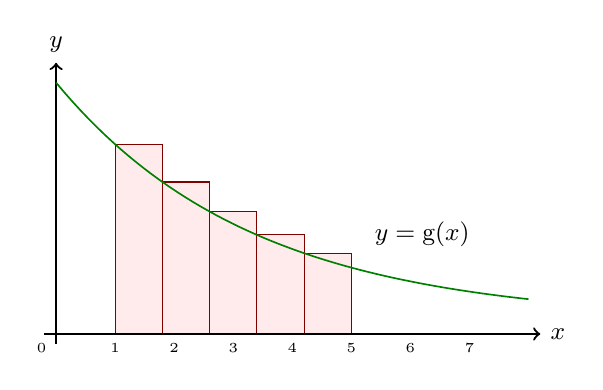
\begin{tikzpicture}[x=0.75cm,y=0.42cm,font=\small]
\foreach \k in {1,1.8,2.6,3.4,4.2}{\fill[red!8,draw=red!50!black,thin] (\k,0) rectangle ({\k+0.8},{8*exp(-0.3*\k)*0.9+0.4});}
\draw[->,thick] (-0.2,0)--(8.2,0) node[right]{$x$}; \draw[->,thick] (0,-0.3)--(0,8.2) node[above]{$y$};
\draw[green!50!black,semithick,domain=0:8,samples=60] plot (\x,{8*exp(-0.3*\x)*0.9+0.4});
\node at (6.2,3.0){$y=\mathrm{g}(x)$};
\foreach \k in {1,...,7}{\node[below,font=\tiny] at (\k,0){$\k$};}\node[below left,font=\tiny] at (0,0){$0$};
\end{tikzpicture}}
\newcommand{\figASRJC}[1]{% 0 question, 1 solution (a), 2 solution (b)
\begin{tikzpicture}[scale=0.9,font=\small]
\ifnum#1<2 \fill[gray!45] plot[domain=-2:1,samples=60](\x,{sqrt(4-\x*\x)})--plot[domain=1:-2](\x,{(\x+2)/sqrt(3)})--cycle;\fi
\ifnum#1=2 \fill[pattern=north east lines,pattern color=blue!70!black] plot[domain=1:2,samples=40](\x,{sqrt(4-\x*\x)})--(2,{4/sqrt(3)})--cycle;
\draw[densely dotted](0,{4/sqrt(3)})--(2,{4/sqrt(3)});\draw[densely dotted](0,{sqrt(3)})--(1,{sqrt(3)});\draw(2,0)--(2,{4/sqrt(3)});
\node[left] at (0,{4/sqrt(3)}){$\frac{4}{\sqrt3}$};\node[left] at (0,1.62){$\sqrt3$};\node[below right] at (2,0){$2$};\node[below left] at (0,0){$0$};\fi
\draw[->](-3,0)--(3.6,0) node[right]{$x$}; \draw[->](0,-2.6)--(0,3) node[above]{$y$};
\draw[thick] (0,0) circle (2);
\draw[thick,domain=-3.2:3.2] plot (\x,{(\x+2)/sqrt(3)}) node[right]{$\sqrt3y=x+2$};
\node at (1.7,-1.6){$x^{2}+y^{2}=4$};
\ifnum#1=0 \node[above] at (0.4,2.1){$\left(1,\sqrt3\right)$};\fi
\ifnum#1=1 \node[above] at (0.4,2.1){$\left(1,\sqrt3\right)$};\draw[densely dotted](1,0)--(1,{sqrt(3)});\node[below] at (1,0){$1$};\node[below left] at (-2,0){$-2$};\fi
\end{tikzpicture}}
\newcommand{\figTJC}{\begin{tikzpicture}[x=0.9cm,y=0.7cm,font=\small]
\fill[pattern=north east lines,pattern color=blue!70!black] (0,0)--(0,pi)--(2,pi)--plot[domain=2:4,samples=60](\x,{acos(\x-3)*pi/180})--(4,0)--cycle;
\draw[->,thick,blue!60!black] (-1.2,0)--(5,0); \draw[->,thick,blue!60!black] (0,-1.2)--(0,4);
\draw[thick] (2,pi)--plot[domain=2:4,samples=60](\x,{acos(\x-3)*pi/180});
\draw (0,pi)--(2,pi); \draw[densely dashed] (2,0)--(2,pi);
\node[left,font=\scriptsize] at (0,pi){$\pi$}; \node[below,font=\scriptsize] at (2,0){$2$}; \node[below,font=\scriptsize] at (4,0){$4$};
\end{tikzpicture}}
%% ============================================================ 121 2021 A-level P2 Q2 (soln: Raffles Institution "Solution for 2021 A-Level Paper 2", /workspace/tmp_ch10/RI_TYS_2021_AL_P2_sol.pdf pp3-4)
\defQ{121}{}{%
The diagram shows a sketch of the curve $y=\mathrm{f}(x)$. The region under the curve between $x=1$ and $x=5$, shown shaded in the diagram, is $A$. This region is split into 5 vertical stripes of equal width, $h$.
\begin{center}\figALstrips{1}\end{center}
\begin{qparts}
\pt{(a)} State the value of $h$ and show, using a sketch, that $\displaystyle\sum_{n=0}^{4}\left(\mathrm{f}\left(1+nh\right)\right)h$ is less than the area of $A$. \mk{2}
\pt{(b)} Find a similar expression that is greater than the area of $A$. \mk{1}
\end{qparts}
You are now given that $\mathrm{f}\left(x\right)=\dfrac{1}{20}x^{2}+1$.
\begin{qparts}
\pt{(c)} Use the expression given in part \textbf{(a)} and your expression from part \textbf{(b)} to find lower and upper bounds for the area of $A$. \mk{2}
\pt{(d)} Sketch the graph of a function $y=\mathrm{g}\left(x\right)$, between $x=1$ and $x=5$, for which the area between the curve, the $x$-axis and the lines $x=1$ and $x=5$ is less than $\displaystyle\sum_{n=0}^{4}\left(\mathrm{g}\left(1+nh\right)\right)h$. \mk{1}
\end{qparts}
\src{2021 A-level P2 Q2}}
\defS{121}{%
\begin{gtpart}{(a)}{2}The value of $h=\dfrac{5-1}{5}=\dfrac{4}{5}$.
\begin{center}\adjustbox{max width=\linewidth}{\figALstrips{2}}\end{center}
[ Note that
\begin{topalign}
\sum_{n=0}^{4}\left(\mathrm{f}(1+nh)\right)h&=h\mathrm{f}(1)+h\mathrm{f}(1+h)+h\mathrm{f}(1+2h)\\
&\quad+h\mathrm{f}(1+3h)+h\mathrm{f}(1+4h)
\end{topalign}
$h\mathrm{f}(1)$ represents the area of left-most rectangle in the diagram above. Similarly, $h\mathrm{f}(1+h)$ represents the area of second left-most rectangle in the diagram above, and $h\mathrm{f}(1+4h)$ represents the area of right-most rectangle in the diagram above.\par
So, $\displaystyle\sum_{n=0}^{4}\left(\mathrm{f}(1+nh)\right)h$ represents the sum of the area of the 5 shaded rectangles. Clearly, the total area of the rectangles is less than the area of $A$. ]\end{gtpart}
\begin{gtpart}{(b)}{1}A similar expression is $\displaystyle\sum_{n=1}^{5}\left(\mathrm{f}(1+nh)\right)h$ or $\displaystyle\sum_{n=0}^{4}\left(\mathrm{f}\left(1+\left(n+1\right)h\right)\right)h$\end{gtpart}
\begin{gtpart}{(c)}{2}\cmtrow[2mm]{\small Note that you can use the GC to evaluate the sum}{\begin{topalign}
\mathrm{f}(x)&=\frac{1}{20}x^{2}+1.
\end{topalign}
\begin{topalign}
\text{Lower bound for area of }A&=\sum_{n=0}^{4}\left(\mathrm{f}(1+nh)\right)h\\
&=\frac45\sum_{n=0}^{4}\left(\frac{1}{20}\left(1+\frac45n\right)^{2}+1\right)=5.608\\
\text{Upper bound for area of }A&=\sum_{n=1}^{5}\left(\mathrm{f}(1+nh)\right)h\\
&=\frac45\sum_{n=1}^{5}\left(\frac{1}{20}\left(1+\frac45n\right)^{2}+1\right)\\
&=6.568
\end{topalign}}\end{gtpart}
\begin{gtpart}{(d)}{1}\begin{center}\adjustbox{max width=\linewidth}{\figALg}\end{center}\end{gtpart}}
%% ============================================================ 122 ASRJC 2025 Prelim P1 Q7 (soln: ASRJC_2025_H2_Math_Prelim_P1_Solutions.pdf pp12-14, official)
\defQ{122}{}{%
Curve $C$ is a circle with radius 2 and center at the origin with equation $x^{2}+y^{2}=4$. Line $L$ has the equation $\sqrt3y=x+2$. The diagram below shows the shaded region $A$ which is enclosed between $C$ and $L$.
\begin{center}\figASRJC{0}\end{center}
\begin{qparts}
\pt{(a)} Use the substitution $x=2\sin\theta$ to show that the area of region $A$ can be written in the expression $\displaystyle\int_{b}^{a}4\cos^{2}\theta\,\dD\theta-c$, where $a$, $b$ and $c$ are exact constants to be determined.\par Hence evaluate this area exactly. \mk{6}
\pt{(b)} The region $B$ is bounded by the curve $C$, the line $L$ and the line $x=2$. Find the volume generated when region $B$ is rotated through $2\pi$ radians about the $y$-axis. Give your answer to two decimal places. \mk{3}
\end{qparts}
\src{ASRJC 2025 Prelim P1 Q7}}
\defS{122}{%
\begin{gtpart}{(a)}{6}\begin{center}\adjustbox{max width=\linewidth}{\figASRJC{1}}\end{center}
The circle $x^{2}+y^{2}=4$ and line $\sqrt3y=x+2$ intersects at $x=-2$ and $x=1$
\begin{topalign}
\text{Area of region }A&=\int_{-2}^{1}\sqrt{4-\left(x\right)^{2}}\,\dD x-\text{area of triangle}\\
x=2\sin\theta\quad&\Rightarrow\quad\frac{\dD x}{\dD\theta}=2\cos\theta
\end{topalign}
When $x=1\ \Rightarrow\ \theta=\sin^{-1}\left(\dfrac12\right)=\dfrac{\pi}{6}$\par
When $x=-2\ \Rightarrow\ \theta=\sin^{-1}\left(-1\right)=-\dfrac{\pi}{2}$
\begin{topalign}
&=\int_{-\frac{\pi}{2}}^{\frac{\pi}{6}}\sqrt{4-\left(2\sin\theta\right)^{2}}\left(2\cos\theta\right)\dD\theta-\frac12\left(3\right)\sqrt3\\
&=\int_{-\frac{\pi}{2}}^{\frac{\pi}{6}}\left(2\cos\theta\right)\left(2\cos\theta\right)\dD\theta-\frac{3\sqrt3}{2}\\
&=\int_{-\frac{\pi}{2}}^{\frac{\pi}{6}}4\cos^{2}\theta\,\dD\theta-\frac{3\sqrt3}{2}\ \text{(shown)}
\end{topalign}
Where $a=\dfrac{\pi}{6},b=-\dfrac{\pi}{2},c=\dfrac{3\sqrt3}{2}$
\begin{topalign}
4\int_{-\frac{\pi}{2}}^{\frac{\pi}{6}}\cos^{2}\theta\,\dD\theta&=4\int_{-\frac{\pi}{2}}^{\frac{\pi}{6}}\left(\frac{\cos2\theta+1}{2}\right)\dD\theta\\
&=2\int_{-\frac{\pi}{2}}^{\frac{\pi}{6}}\left(\cos2\theta+1\right)\dD\theta\\
&=2\left[\frac{\sin2\theta}{2}+\theta\right]_{-\frac{\pi}{2}}^{\frac{\pi}{6}}
\end{topalign}
\begin{topalign}
\text{Required area}&=2\left[\left(\frac12\sin2\left(\frac{\pi}{6}\right)+\frac{\pi}{6}\right)-\left(\frac12\sin2\left(-\frac{\pi}{2}\right)-\frac{\pi}{2}\right)\right]-\frac{3\sqrt3}{2}\\
&=\left(2\left(\frac{\sqrt3}{4}+\frac{\pi}{6}+\frac{\pi}{2}\right)\right)-\frac{3\sqrt3}{2}\\
&=\frac{\sqrt3}{2}+\frac{4\pi}{3}-\frac{3\sqrt3}{2}=\frac{4\pi}{3}-\sqrt3
\end{topalign}\end{gtpart}
\begin{gtpart}{(b)}{3}\begin{center}\adjustbox{max width=\linewidth}{\figASRJC{2}}\end{center}
Volume obtained by rotating region $B$ through $2\pi$ radians about $y$-axis
\begin{topalign}
&=\text{volume of cylinder}-\pi\int_{\sqrt3}^{\frac{4}{\sqrt3}}\left(\sqrt3y-2\right)^{2}\dD y-\pi\int_{0}^{\sqrt3}\left(4-y^{2}\right)\dD y\\
&=\pi\left(2\right)^{2}\left(\frac{4}{\sqrt3}\right)-\pi\int_{\sqrt3}^{\frac{4}{\sqrt3}}\left(\sqrt3y-2\right)^{2}\dD y-\pi\int_{0}^{\sqrt3}\left(4-y^{2}\right)\dD y\\
&\approx8.4644\\
&\approx8.46\ \text{(2 d.p.)}
\end{topalign}\end{gtpart}}
%% ============================================================ 123 TJC 2025 Prelim P1 Q10 (soln: TJC_2025_H2_Math_Prelim_P1_Solutions.pdf pp11-12, official)
\defQ{123}{}{%
\begin{qparts}
\pt{(a)} Differentiate $\sqrt{1-x^{2}}$ with respect to $x$.\par Hence evaluate $\displaystyle\int_{-1}^{1}\cos^{-1}x\,\dD x$, giving your answer in exact form. \mk{5}
\pt{(b)} The finite region $R$ is bounded by the curve $y=\cos^{-1}\left(x-3\right)$, where $2\leqslant x\leqslant4$, the line $y=\pi$ and the axes.
\begin{qparts}[2.2em]
\pt{(i)} Describe a geometrical transformation which will map the graph of $y=\cos^{-1}\left(x-3\right)$ onto the graph of $y=\cos^{-1}x$. \mk{1}
\pt{(ii)} Hence or otherwise, find the area of $R$ in exact form. \mk{2}
\end{qparts}
\pt{(c)} Find the exact value of the volume generated when $R$ is rotated completely about the $y$-axis. \mk{4}
\end{qparts}
\src{TJC 2025 Prelim P1 Q10}}
\defS{123}{%
\begin{gtpart}{(a)}{5}\begin{topalign}
\frac{\dD}{\dD x}\sqrt{1-x^{2}}&=\frac{-2x}{2\sqrt{1-x^{2}}}=-\frac{x}{\sqrt{1-x^{2}}}\\
\int_{-1}^{1}\cos^{-1}x\,\dD x&=\Big[x\cos^{-1}x\Big]_{-1}^{1}-\int_{-1}^{1}x\left[-\frac{1}{\sqrt{1-x^{2}}}\right]\dD x\\
&=1(0)-(-1)(\pi)-\int_{-1}^{1}\frac12\cdot\frac{-2x}{\sqrt{1-x^{2}}}\,\dD x\\
&=\pi-\left[\sqrt{1-x^{2}}\right]_{-1}^{1}\\
&=\pi-0\\
&=\pi
\end{topalign}\end{gtpart}
\begin{gtpart}{(b)(i)}{1}Translate the graph of $y=\cos^{-1}(x-3)$ three units in the negative direction of $x$-axis to obtain the graph of $y=\cos^{-1}x$\end{gtpart}
\begin{gtpart}{(b)(ii)}{2}\begin{center}\figTJC\end{center}
\begin{topalign}
\text{Area of the region }R&=\left(2\right)\left(\pi\right)+\int_{2}^{4}\cos^{-1}\left(x-3\right)\dD x\\
&=2\pi+\int_{-1}^{1}\cos^{-1}u\,\dD u\\
&=3\pi
\end{topalign}
Alternative Method:
\begin{topalign}
\text{Area of the region }R&=\int_{0}^{\pi}3+\cos y\,\dD y\\
&=\Big[3x+\sin y\Big]_{0}^{\pi}\\
&=3\pi
\end{topalign}\end{gtpart}
\begin{gtpart}{(c)}{4}\begin{center}\figTJC\end{center}
Volume generated when rotated completely about $y$-axis
\begin{topalign}
&=\pi\int_{0}^{\pi}x^{2}\,\dD y\\
&=\pi\int_{0}^{\pi}\left(\cos y+3\right)^{2}\dD y\\
&=\pi\int_{0}^{\pi}\left(\cos^{2}y+6\cos y+9\right)\dD y\\
&=\pi\int_{0}^{\pi}\left[\frac12\left(\cos2y+1\right)+6\cos y+9\right]\dD y\\
&=\pi\left[\frac14\sin2y+6\sin y+\frac{19}{2}y\right]_{0}^{\pi}\\
&=\frac{19}{2}\pi^{2}
\end{topalign}\end{gtpart}}
\providecommand{\dD}{\mathrm{d}}
%% ---------------- figures (TikZ redraws of the answer-sheet graphs)
\newcommand{\figRIcurrent}{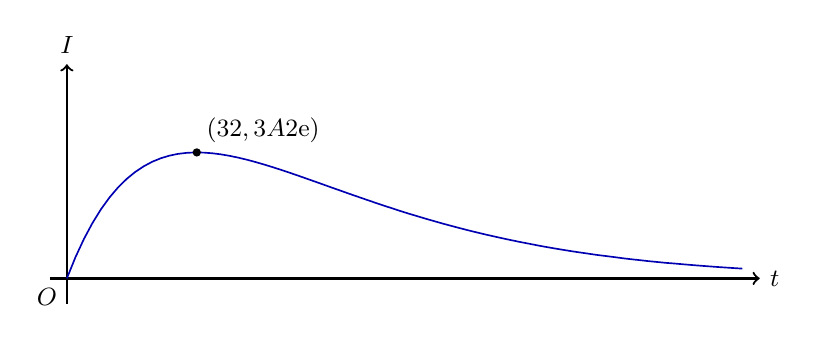
\begin{tikzpicture}[x=1.1cm,y=1.6cm,font=\small]
\draw[->,thick](-0.2,0)--(8,0) node[right]{$t$};\draw[->,thick](0,-0.2)--(0,1.7) node[above]{$I$};
\draw[blue!70!black,semithick,domain=0:7.8,samples=80] plot(\x,{2.718*\x*exp(-2*\x/3)/1.5});
\fill (1.5,1) circle(1.5pt) node[above right]{$\left(\dfrac32,\dfrac{3A}{2\mathrm{e}}\right)$};
\node[below left] at (0,0){$O$};
\end{tikzpicture}}
\newcommand{\figNJCpressure}{\begin{tikzpicture}[x=0.075cm,y=0.022cm,font=\small]
\draw[->,thick](-3,0)--(95,0) node[right]{$h$};\draw[->,thick](0,-8)--(0,140) node[above]{$P$};
\draw[semithick,domain=0:88,samples=120] plot(\x,{101.3*((abs(293-6.5*\x)/293)^5.2015)});
\node[left] at (0,101.3){$101300$};\node[below left] at (0,0){$O$};\node[below] at (45.1,0){$45.1$};
\end{tikzpicture}}
%% ============================================================ 131 HCI 2025 Prelim P1 Q10 (soln: HCI_2025_H2_Math_Prelim_P1_Solutions.pdf pp16-18, official)
\defQ{131}{}{%
\begin{qparts}
\pt{(a)} Express $\dfrac{1}{Q\left(500-Q\right)}$ in partial fractions. \mk{2}
\pt{(b)} A group of scientists is monitoring the population of a particular species of birds on an island. At time $t$ years after the start of the monitoring, the number of birds on the island is $Q$. The scientists observe that the birth rate is proportional to the bird's population and the birds are dying at a rate proportional to the square of the bird's population. There were 1000 birds on the island when the scientists first started monitoring the population. They discover that the population remains unchanged when there are 500 birds.
\begin{qparts}
\pt{(i)} Show that the differential equation relating $Q$ and $t$ is given by
\[\frac{\dD Q}{\dD t}=kQ\left(500-Q\right),\]
where $k$ is a positive constant. \mk{2}
\pt{(ii)} Hence, solve the differential equation, expressing $Q$ in terms of $k$ and $t$. \mk{5}
\end{qparts}
\end{qparts}
\src{HCI 2025 Prelim P1 Q10}}
\defS{131}{%
\begin{gtpart}{(a)}{2}\begin{topalign}
\frac{1}{Q\left(500-Q\right)}&=\frac{A}{Q}+\frac{B}{500-Q}=\frac{\left(500-Q\right)A+BQ}{Q\left(500-Q\right)}\\
\Rightarrow1&=A\left(500-Q\right)+BQ
\end{topalign}
For $Q=0$, $1=500A\Rightarrow A=\dfrac{1}{500}$.\par
For $Q=500$, $1=500B\Rightarrow B=\dfrac{1}{500}$.
\begin{topalign}
\therefore\frac{1}{Q\left(500-Q\right)}&=\frac{1}{500Q}+\frac{1}{500\left(500-Q\right)}
\end{topalign}\end{gtpart}
\begin{gtpart}{(b)(i)}{2}Increase rate $\propto Q$\par
$\Rightarrow$ Increase rate $=aQ$ ($a$ is the constant of proportionality for increase rate)\par\smallskip
Decrease rate $\propto Q^{2}$\par
$\Rightarrow$ \fhl{Decrease rate} $=bQ^{2}$ ($b$ is the constant of proportionality for decrease rate)
\begin{topalign}
\therefore\frac{\dD Q}{\dD t}&=aQ-bQ^{2}\quad\text{(Increase rate -- Decrease rate)}
\end{topalign}
$\dfrac{\dD Q}{\dD t}=0$ when $Q=500$
\begin{topalign}
\Rightarrow500a-250000b&=0\\
\Rightarrow a&=500b\\
\therefore\frac{\dD Q}{\dD t}&=500bQ-bQ^{2}\\
\Rightarrow\frac{\dD Q}{\dD t}&=kQ\left(500-Q\right)\quad\text{where }k=b
\end{topalign}\end{gtpart}
\begin{gtpart}{(b)(ii)}{5}\begin{topalign}
\int\frac{1}{Q\left(500-Q\right)}\,\dD Q&=\int k\,\dD t\\
\frac{1}{500}\int\frac1Q+\frac{1}{500-Q}\,\dD Q&=\int k\,\dD t\quad\text{(from part (a))}\\
\frac{1}{500}\Big[\ln Q-\ln\left|500-Q\right|\Big]&=kt+C\\
\ln\left|\frac{Q}{500-Q}\right|&=500kt+500C
\end{topalign}
\textbf{Resolving the modulus}:\par\smallskip
\underline{\textbf{Method 1 (using arbitrary constant):}}
\begin{topalign}
\ln\left|\frac{Q}{500-Q}\right|&=500kt+500C\\
\Rightarrow\left|\frac{Q}{500-Q}\right|&=\mathrm{e}^{500kt+500C}\\
\Rightarrow\frac{Q}{500-Q}&=\pm\mathrm{e}^{500C}\mathrm{e}^{500kt}\\
\Rightarrow\frac{Q}{500-Q}&=H\mathrm{e}^{500kt},\quad\text{where }H=\pm\mathrm{e}^{500C}\text{ is an arbitrary constant}
\end{topalign}
Therefore, we have
\begin{topalign}
Q&=500H\mathrm{e}^{500kt}-QH\mathrm{e}^{500kt}\\
Q&=\frac{500H\mathrm{e}^{500kt}}{1+H\mathrm{e}^{500kt}}
\end{topalign}
When $t=0$, $Q=1000$
\begin{topalign}
\frac{1000}{500-1000}&=H\Rightarrow H=-2\\
\therefore Q&=\frac{-1000\mathrm{e}^{500kt}}{1-2\mathrm{e}^{500kt}}\\
\Rightarrow Q&=\frac{1000\mathrm{e}^{500kt}}{2\mathrm{e}^{500kt}-1}
\end{topalign}
\underline{\textbf{Method 2 (using the initial condition):}}\par
When $t=0$, $Q=1000$, and $Q$ stabilized at 500 given in the question.\par
Therefore $Q\geq500\Rightarrow Q-500\geq0$
\begin{topalign}
\Rightarrow\ln\left|\frac{Q}{500-Q}\right|&=\ln\left(\frac{Q}{Q-500}\right)
\end{topalign}
Hence we have
\begin{topalign}
\ln\left(\frac{Q}{Q-500}\right)&=500kt+500C=500kt+D
\end{topalign}
When $t=0$, $Q=1000$
\begin{topalign}
\ln\left(\frac{1000}{1000-500}\right)&=0+D\\
\Rightarrow D&=\ln2\\
\ln\left(\frac{Q}{Q-500}\right)&=500kt+\ln2\\
\frac{Q}{Q-500}&=\mathrm{e}^{500kt+\ln2}\\
\frac{Q}{Q-500}&=\mathrm{e}^{\ln2}\mathrm{e}^{500kt}=2\mathrm{e}^{500kt}\\
Q&=2\mathrm{e}^{500kt}\left(Q-500\right)\\
Q-2\mathrm{e}^{500kt}Q&=-1000\mathrm{e}^{500kt}\\
Q&=\frac{-1000\mathrm{e}^{500kt}}{1-2\mathrm{e}^{500kt}}\\
Q&=\frac{1000\mathrm{e}^{500kt}}{2\mathrm{e}^{500kt}-1}
\end{topalign}\end{gtpart}}
%% ============================================================ 132 HCI 2025 Prelim P1 Q3 (soln: HCI_2025_H2_Math_Prelim_P1_Solutions.pdf p4, official)
\defQ{132}{}{%
It is given that $\left(2xy\dfrac{\dD y}{\dD x}+y^{2}\right)\cos x=\dfrac{1}{xy^{2}}$, where $0<x<\dfrac{\pi}{2}$ and $y\neq0$.
\begin{qparts}
\pt{(a)} Using the substitution $u=xy^{2}$, show that the differential equation can be reduced to $\dfrac{\dD u}{\dD x}=\dfrac{\sec x}{u}$. \mk{3}
\pt{(b)} Hence find the general solution to the differential equation. \mk{3}
\end{qparts}
\src{HCI 2025 Prelim P1 Q3}}
\defS{132}{%
\begin{gtpart}{(a)}{3}\begin{topalign}
u&=xy^{2}\\
\frac{\dD u}{\dD x}&=y^{2}+x\left(2y\frac{\dD y}{\dD x}\right)\\
\cos x\left(y^{2}+2xy\frac{\dD y}{\dD x}\right)&=\frac{1}{xy^{2}}\\
\cos x\left(\frac{\dD u}{\dD x}\right)&=\frac1u\\
\frac{\dD u}{\dD x}&=\frac{\sec x}{u}
\end{topalign}\end{gtpart}
\begin{gtpart}{(b)}{3}\begin{topalign}
\int u\,\dD u&=\int\sec x\,\dD x\\
\frac12u^{2}&=\ln\left(\sec x+\tan x\right)+C\quad\left(\because\sec x,\tan x>0\text{ for }0<x<\frac{\pi}{2}\right)\\
x^{2}y^{4}&=2\ln\left(\sec x+\tan x\right)+\fhlmi{D}
\end{topalign}\end{gtpart}}
%% ============================================================ 133 2018 A-level P1 Q10 (soln: Raffles Institution "Solution for 2018 A-Level Paper 1" pp10-11, grail.moe/library/9387; question paper not obtainable)
\defQ{133}{}{%
\fhlp{An electrical circuit comprises a power source of $V$ volts in series with a resistance of $R$ ohms, a capacitance of $C$ farads and an inductance of $L$ henries. The current in the circuit, $t$ seconds after turning on the power, is $I$ amps and the charge on the capacitor is $q$ coulombs. The circuit can be used by scientists to investigate resonance, to model heavily damped motion and to tune into radio stations on a stereo tuner. It is given that $R$, $C$ and $L$ are constants, and that $I=0$ when $t=0$.}\par\smallskip
\fhlp{A differential equation for the circuit is $L\dfrac{\dD I}{\dD t}+RI+\dfrac{q}{C}=V$, where $I=\dfrac{\dD q}{\dD t}$.}
\begin{qparts}
\pt{(i)} \fhlp{Show that, under certain conditions on $V$ which should be stated,
\[L\dfrac{\dD^{2}I}{\dD t^{2}}+R\dfrac{\dD I}{\dD t}+\dfrac{I}{C}=0.\]} \mk{2}
\end{qparts}
\fhlp{It is now given that the differential equation in part (i) holds for the rest of the question.}
\begin{qparts}
\pt{(ii)} \fhlp{Given that $I=At\mathrm{e}^{-\frac{Rt}{2L}}$ is a solution of the differential equation, where $A$ is a positive constant, show that $C=\dfrac{4L}{R^{2}}$.} \mk{5}
\pt{(iii)} \fhlp{In a particular circuit, $R=4$, $L=3$ and $C=0.75$. Find the maximum value of $I$ in terms of $A$, showing that this value is a maximum.} \mk{4}
\pt{(iv)} \fhl{Sketch the graph of $I$ against $t$.} \mk{2}
\end{qparts}
\src{2018 A-level P1 Q10}}
\defS{133}{%
\begin{gtpart}{}{}\begin{topalign}
L\frac{\dD I}{\dD t}+RI+\frac{q}{C}&=V,\quad\text{where }I=\frac{\dD q}{\dD t}
\end{topalign}\end{gtpart}
\begin{gtpart}{(i)}{}Differentiate with respect to $t$,
\begin{topalign}
L\frac{\dD^{2}I}{\dD t^{2}}+R\frac{\dD I}{\dD t}+\frac1C\frac{\dD q}{\dD t}&=\frac{\dD V}{\dD t}\\
L\frac{\dD^{2}I}{\dD t^{2}}+R\frac{\dD I}{\dD t}+\frac{I}{C}&=\frac{\dD V}{\dD t},\quad\text{since }I=\frac{\dD q}{\dD t}
\end{topalign}
Therefore,
\begin{topalign}
L\frac{\dD^{2}I}{\dD t^{2}}+R\frac{\dD I}{\dD t}+\frac{I}{C}&=0,\quad\text{when }\frac{\dD V}{\dD t}=0\text{ that is, }V\text{ is a constant.}
\end{topalign}\end{gtpart}
\begin{gtpart}{(ii)}{}\begin{topalign}
I&=At\mathrm{e}^{-\frac{Rt}{2L}}\\
\frac{\dD I}{\dD t}&=A\mathrm{e}^{-\frac{Rt}{2L}}+At\mathrm{e}^{-\frac{Rt}{2L}}\left(-\frac{R}{2L}\right)=A\mathrm{e}^{-\frac{Rt}{2L}}-\frac{AR}{2L}t\mathrm{e}^{-\frac{Rt}{2L}}\\
\frac{\dD^{2}I}{\dD t^{2}}&=-\frac{AR}{2L}\mathrm{e}^{-\frac{Rt}{2L}}-\frac{AR}{2L}\mathrm{e}^{-\frac{Rt}{2L}}+\frac{AR^{2}}{4L^{2}}t\mathrm{e}^{-\frac{Rt}{2L}}=-\frac{AR}{L}\mathrm{e}^{-\frac{Rt}{2L}}+\frac{AR^{2}}{4L^{2}}t\mathrm{e}^{-\frac{Rt}{2L}}
\end{topalign}
Sub into $L\dfrac{\dD^{2}I}{\dD t^{2}}+R\dfrac{\dD I}{\dD t}+\dfrac{I}{C}=0$,
\begin{topalign}
-AR\mathrm{e}^{-\frac{Rt}{2L}}+\frac{AR^{2}}{4L}t\mathrm{e}^{-\frac{Rt}{2L}}+AR\mathrm{e}^{-\frac{Rt}{2L}}-\frac{AR^{2}}{2L}t\mathrm{e}^{-\frac{Rt}{2L}}+\frac{A}{C}t\mathrm{e}^{-\frac{Rt}{2L}}&=0\\
-AR\mathrm{e}^{-\frac{Rt}{2L}}+AR\mathrm{e}^{-\frac{Rt}{2L}}+\frac{AR^{2}}{4L}t\mathrm{e}^{-\frac{Rt}{2L}}-\frac{AR^{2}}{2L}t\mathrm{e}^{-\frac{Rt}{2L}}+\frac{A}{C}t\mathrm{e}^{-\frac{Rt}{2L}}&=0\\
-\frac{R^{2}}{4L}+\frac1C=0\Rightarrow C&=\frac{4L}{R^{2}}
\end{topalign}\end{gtpart}
\begin{gtpart}{(iii)}{}\cmtrow{\small By right, we should sub $R=4$, $L=3$ and $C=0.75$ into $I$ and check that it still a solution of the DE.}{Note that the given values satisfy (ii),\par
when $R=4$ and $L=3$, from (ii), $C=\dfrac{4L}{R^{2}}=\dfrac34$
\begin{topalign}
I&=At\mathrm{e}^{-\frac23t}\\
\frac{\dD I}{\dD t}=0\ &\Rightarrow\ A\mathrm{e}^{-\frac23t}-\frac{2A}{3}t\mathrm{e}^{-\frac23t}=0\\
&\Rightarrow\ t=\frac32\\
I&=\frac{3A}{2\mathrm{e}}
\end{topalign}
Sub into $L\dfrac{\dD^{2}I}{\dD t^{2}}+R\dfrac{\dD I}{\dD t}+\dfrac{I}{C}=0$,
\begin{topalign}
3\frac{\dD^{2}I}{\dD t^{2}}+4\left(0\right)+\frac{1}{0.75}\cdot\frac{3A}{2\mathrm{e}}&=0\\
\frac{\dD^{2}I}{\dD t^{2}}&=-\frac{A}{1.5\mathrm{e}}<0
\end{topalign}}\end{gtpart}
\begin{gtpart}{(iv)}{}\begin{center}\adjustbox{max width=\linewidth}{\figRIcurrent}\end{center}
Remember to label the max point $\left(\dfrac32,\dfrac{3A}{2\mathrm{e}}\right)$\end{gtpart}}
%% ============================================================ 134 NJC 2025 Prelim P2 Q4 (soln: NJC_2025_H2_Math_Prelim_P2_Solutions.pdf pp8-9, official)
\defQ{134}{}{%
The rate of decrease of atmospheric pressure $P$ Pascals (Pa) with respect to altitude $h$ kilometres above sea level, is proportional to $\dfrac{P}{T}$, where $T$ is the temperature measured in Kelvin (K). The temperature $T$ decreases linearly by 6.5 K for every one-kilometre increase in the altitude above sea level. It is given that the temperature is 293 K at sea level.
\begin{qparts}
\pt{(i)} Find a differential equation for $\dfrac{\dD P}{\dD h}$ in terms of $P$ and $h$. \mk{2}
\pt{(ii)} Given that $P>0$, solve this model in part (i) to show that
\[P=A\left|293-6.5h\right|^{b},\ \text{where }A\text{ and }b\text{ are constants.}\]
Explain whether $b$ is positive or negative. \mk{4}
\end{qparts}
It is given that the atmospheric pressures are 101\,300 Pa at sea level and 80\,000 Pa at $h=2$.
\begin{qparts}
\pt{(iii)} Find the atmospheric pressure at the top of Mount Everest with an altitude of 8848 metres. \mk{4}
\pt{(iv)} For $h\geq0$, sketch the graph of $P$ against $h$. Explain a limitation of this model. \mk{3}
\end{qparts}
\src{NJC 2025 Prelim P2 Q4}}
\defS{134}{%
\begin{gtpart}{(i)}{2}\begin{topalign}
\frac{\dD P}{\dD h}&=-k\left(\frac{P}{T}\right)\\
T&=293-6.5h\\
\frac{\dD P}{\dD h}&=\frac{-kP}{293-6.5h},\quad\text{where }k>0\\
\text{or }\frac{\dD P}{\dD h}&=\frac{kP}{293-6.5h},\quad\text{where }k<0
\end{topalign}\end{gtpart}
\begin{gtpart}{(ii)}{4}\begin{topalign}
\frac1P\frac{\dD P}{\dD h}&=-\frac{k}{293-6.5h}\\
\int\frac1P\,\dD P&=\int-\frac{k}{293-6.5h}\,\dD h
\end{topalign}
Since $P>0$,
\begin{topalign}
\ln P&=\frac{k}{6.5}\ln\left|293-6.5h\right|+C\\
P&=\mathrm{e}^{\frac{k}{6.5}\ln\left|293-6.5h\right|+C}\\
&=A\left[\mathrm{e}^{\ln\left|293-6.5h\right|}\right]^{\frac{k}{6.5}},\quad\text{where }A=\mathrm{e}^{C}\\
&=A\left|293-6.5h\right|^{\frac{k}{6.5}}\\
&=A\left|293-6.5h\right|^{b}
\end{topalign}
Since $k>0$, $b=\dfrac{k}{6.5}>0$.\end{gtpart}
\begin{gtpart}{(iii)}{4}When $h=0$, $P=101300$,
\begin{topalign}
101300&=A\left(293^{b}\right)\quad\ldots(1)
\end{topalign}
When $h=2$, $P=80000$,
\begin{topalign}
80000&=A\left(293-6.5\times2\right)^{b}\\
80000&=A\left(280^{b}\right)\quad\ldots(2)
\end{topalign}
$(1)/(2)$,
\begin{topalign}
\frac{101300}{80000}&=\left(\frac{293}{280}\right)^{b}\\
b&=\frac{\ln\frac{101300}{80000}}{\ln\frac{293}{280}}\\
&=5.2015\ \text{(5 s.f.)}\\
A&=\frac{101300}{293^{5.2015}}\\
&=1.4935\times10^{-8}\\
P&=1.4935\times10^{-8}\left|293-6.5h\right|^{5.2015}
\end{topalign}
When $h=8.848$,
\begin{topalign}
P&=1.4935\times10^{-8}\left|293-6.5\left(8.848\right)\right|^{5.2015}\\
&=32500\ \text{(to 3 s.f.)}
\end{topalign}
The atmospheric pressure is 32\,500 Pascals.\end{gtpart}
\begin{gtpart}{(iv)}{3}\begin{center}\adjustbox{max width=\linewidth}{\figNJCpressure}\end{center}
\textbf{Either}\par
The model suggests that when altitude is greater than 45.1 km, \fhl{atmospheric} pressure increases (to infinity) as altitude increases, which is not possible.\par\smallskip
\textbf{Or}\par
As the temperature $T$ measured in Kelvin can only be positive, the model is invalid if $T=293-6.5h<0$.\end{gtpart}}
%% CH14 COMPLEX NUMBERS EQ
\newcommand{\figTJCsq}{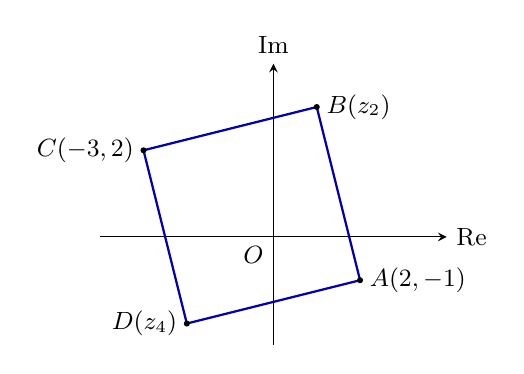
\begin{tikzpicture}[scale=0.55,font=\small,>=stealth]
\draw[->](-4,0)--(4,0)node[right]{Re};\draw[->](0,-2.5)--(0,4)node[above]{Im};\node[below left]at(0,0){$O$};
\draw[blue!70!black,thick](2,-1)--(1,3)--(-3,2)--(-2,-2)--cycle;
\fill(2,-1)circle(2pt)node[right]{$A(2,-1)$};\fill(1,3)circle(2pt)node[right]{$B(z_{2})$};
\fill(-3,2)circle(2pt)node[left]{$C(-3,2)$};\fill(-2,-2)circle(2pt)node[left]{$D(z_{4})$};
\end{tikzpicture}}
\newcommand{\figTJCac}{\begin{tikzpicture}[scale=0.55,font=\small,>=stealth]
\draw[->](-4,0)--(4,0)node[right]{Re$(z)$};\draw[->](0,-2)--(0,3)node[above]{Im$(z)$};\node[below left]at(0,0){$O$};
\fill(2,-1)circle(2pt)node[right]{$A\ (2,-1)$};\fill(-3,2)circle(2pt)node[right]{$C\ (-3,2)$};
\draw[->,blue](0,0)--(2,-1);\draw[->,blue](0,0)--(-3,2);
\end{tikzpicture}}
\newcommand{\figVJCa}[1]{\begin{tikzpicture}[scale=1.1,font=\small]
\draw[->](-1.6,0)--(1.6,0)node[right]{Re};\draw[->](0,-1.5)--(0,2.2)node[above]{Im};\node[below right]at(0,0){$O$};
\draw[dashed](0,0)--(-0.707,0.707)node[midway,below left]{$1$};\draw[dashed](0,0)--(-1.225,-1.225)node[midway,above left]{$\sqrt3$};
\draw[dashed](-0.707,0.707)--(0.518,1.932)node[midway,above left]{$\sqrt3$};#1
\node at(-0.707,0.707){$\times$};\node[left]at(-0.75,0.75){$P$};\node at(-1.225,-1.225){$\times$};\node[below]at(-1.225,-1.3){$Q$};
\node at(0.518,1.932){$\times$};\node[right]at(0.55,1.95){$R$};
\end{tikzpicture}}
%% ===== 141 TJC 2025 Prelim P1 Q8 (soln: TJC_2025_H2_Math_Prelim_P1_Solutions.pdf pp8-9)
\defQ{141}{}{%
\begin{qparts}
\pt{(a)} The complex numbers $z$ and $w$ satisfy the following equations.
\[2z+|w|=2-4\mathrm{i}\qquad\mathrm{i}z-w=2\mathrm{i}\]
Find $z$ and $w$, giving your answers in the form $a+\mathrm{i}b$, where $a$ and $b$ are real numbers. \mk{5}
\pt{(b)} It is given that $z_{1}=2-\mathrm{i}$ and $z_{3}=-3+2\mathrm{i}$. On an Argand diagram, mark the points $A$ and $C$ representing $z_{1}$ and $z_{3}$ respectively. \mk{1}\par
The points $B$ and $D$ on the Argand diagram represent complex numbers $z_{2}$ and $z_{4}$ respectively. Given that $ABCD$ is a square, labelled in an anti-clockwise direction, find $z_{2}$ and $z_{4}$. \mk{4}
\end{qparts}
\src{TJC 2025 Prelim P1 Q8}}
\defS{141}{%
\begin{gtpart}{(a)}{5}\begin{topalign}
2z+\left|w\right|&=2-4\mathrm{i}\quad\text{--- (1)}\\
\mathrm{i}z-w&=2\mathrm{i}\quad\text{--- (2)}
\end{topalign}
From (1): \begin{topalign}z&=\frac{2-4\mathrm{i}-\left|w\right|}{2}\end{topalign}
Substitute into (2):
\begin{topalign}
\mathrm{i}\left(\frac{2-4\mathrm{i}-\left|w\right|}{2}\right)-w&=2\mathrm{i}\\
2\mathrm{i}+4-\mathrm{i}\left|w\right|-2w&=4\mathrm{i}
\end{topalign}
Let $w=a+\mathrm{i}b$, $a,b\in\mathbb{R}$,
\begin{topalign}
2\mathrm{i}+4-\mathrm{i}\sqrt{a^{2}+b^{2}}-2(a+\mathrm{i}b)&=4\mathrm{i}\\
4-2a+\mathrm{i}\left(2-\sqrt{a^{2}+b^{2}}-2b\right)&=4\mathrm{i}
\end{topalign}
Compare real and imaginary parts:
\begin{topalign}
4-2a=0\ \Rightarrow\ a&=2\quad\text{--- (3)}\\
2-\sqrt{a^{2}+b^{2}}-2b&=4\quad\text{--- (4)}
\end{topalign}
Substitute (3) into (4):
\begin{topalign}
-2-2b&=\sqrt{4+b^{2}}\quad\text{--- (5)}\\
\Rightarrow\left(-2-2b\right)^{2}&=4+b^{2}\\
4+8b+4b^{2}&=4+b^{2}\\
b\left(3b+8\right)&=0
\end{topalign}
$\Rightarrow b=0$ (rejected since $\sqrt{4+b^{2}}\neq-2$ from (5)) or $b=-\dfrac83$
\begin{topalign}
\therefore w&=2-\frac83\mathrm{i}\\
z&=\frac{2-4\mathrm{i}-(-2-2b)}{2}=2-2\mathrm{i}+\left(-\frac83\right)=-\frac23-2\mathrm{i}
\end{topalign}\end{gtpart}
\begin{gtpart}{(b)}{5}\begin{center}\figTJCac\end{center}
$\overrightarrow{BA}$ represents the complex number $2-\mathrm{i}-z_{2}$ and $\overrightarrow{BC}$ represents the complex number $-3+2\mathrm{i}-z_{2}$.\par
Since $\angle ABC=\dfrac{\pi}{2}$, $A$ is obtained by rotating $C$ through $90^{\circ}$ in anti-clockwise direction about $B$. i.e.\ $\overrightarrow{BC}$ rotated by $90^{\circ}$ anticlockwise gives $\overrightarrow{BA}$.
\begin{center}\figTJCsq\end{center}
\fhl{{\color{gray}$\overrightarrow{BC}\times\mathrm{i}=\overrightarrow{BA}$}}\par
\begin{topalign}
\mathrm{i}\left(-3+2\mathrm{i}-z_{2}\right)&=2-\mathrm{i}-z_{2}\\
-3\mathrm{i}-2-\mathrm{i}z_{2}&=2-\mathrm{i}-z_{2}\\
\left(1-\mathrm{i}\right)z_{2}&=4+2\mathrm{i}\\
z_{2}&=\frac{4+2\mathrm{i}}{1-\mathrm{i}}\cdot\frac{1+\mathrm{i}}{1+\mathrm{i}}=\frac{2+6\mathrm{i}}{2}=1+3\mathrm{i}\\
\overrightarrow{AB}&=\overrightarrow{DC}\\
1+3\mathrm{i}-(2-\mathrm{i})&=-3+2\mathrm{i}-z_{4}\\
z_{4}&=-3+2\mathrm{i}+1-4\mathrm{i}=-2-2\mathrm{i}
\end{topalign}\end{gtpart}}
%% ===== 142 2025 A-level P1 Q12 (question: Tim Gan Math transcription; soln: VJC 2025 A Level Paper 1 Solutions pp16-17, /workspace/uploads/2025_A_Level_solution Paper 1_Student.pdf)
\defQ{142}{}{%
\textbf{Do not use a calculator in answering this question.}\par
It is given that $1+2\mathrm{i}$ is a complex root of the equation $z^{3}+pz^{2}+qz-10=0$, where $p$ and $q$ are real numbers.
\begin{qparts}
\pt{(a)} State another complex root of the equation in the form $a+\mathrm{i}b$, where $a$ and $b$ are real numbers and $b\neq0$. Justify your answer. \mk{2}
\pt{(b)} Find the values of $p$ and $q$, and find the third root. \mk{6}
\pt{(c)} Hence find the roots of the equation $1+pw+qw^{2}-10w^{3}=0$. \mk{2}
\end{qparts}
\src{2025 A-level P1 Q12}}
\defS{142}{%
\begin{gtpart}{(a)}{2}\fhlp{Since $1+2\mathrm{i}$ is a root and all coefficients of the polynomial are real, $1-2\mathrm{i}$ is another root by conjugate root theorem.}\end{gtpart}
\begin{gtpart}{(b)}{6}\fhlp{\begin{topalign}
z^{3}+pz^{2}+qz-10&=\left(z-(1-2\mathrm{i})\right)\left(z-(1+2\mathrm{i})\right)(z-k)\quad\text{where }k\text{ is real}\\
&=\left((z-1)-2\mathrm{i})\right)\left((z-1)+2\mathrm{i})\right)(z-k)\\
&=\left((z-1)^{2}-(2\mathrm{i})^{2}\right)(z-k)\\
&=\left(z^{2}-2z+5\right)(z-k)
\end{topalign}
\begin{topalign}
&\text{Comparing constants: }-10=5(-k)\ \Rightarrow\ k=2\\
&\text{Comparing }z^{2}\text{: }\ \ \ \ \ \,p=-k-2=-4\\
&\text{Comparing }z\text{: }\ \ \ \ \ \ \ \,q=5+2k=9
\end{topalign}
Hence $p=-4$, $q=9$ and the third root is $2$}\end{gtpart}
\begin{gtpart}{(c)}{2}\fhlp{Note that $w=0$ is not a solution to the equation
\begin{topalign}
1+pw+qw^{2}-10w^{3}&=0
\end{topalign}
Dividing throughout by $w^{3}$
\begin{topalign}
\left(\frac1w\right)^{3}+p\left(\frac1w\right)^{2}+q\left(\frac1w\right)-10&=0
\end{topalign}
\begin{topalign}
\frac1w=1+2\mathrm{i}\quad&\text{or}\quad\frac1w=1-2\mathrm{i}\quad\text{or}\quad\frac1w=2\\
w=\frac{1}{1+2\mathrm{i}}\times\frac{1-2\mathrm{i}}{1-2\mathrm{i}}\quad&\phantom{\text{or}}\quad w=\frac{1}{1-2\mathrm{i}}\times\frac{1+2\mathrm{i}}{1+2\mathrm{i}}\quad\phantom{\text{or}}\quad w=\frac12\\
=\frac15(1-2\mathrm{i})\quad&\phantom{\text{or}}\quad\ \ =\frac15(1+2\mathrm{i})
\end{topalign}}\end{gtpart}}
%% ===== 143 NYJC 2025 Prelim P2 Q2 (soln: NYJC 2025 P2 Marking Guide p1)
\defQ{143}{}{%
\begin{qparts}
\pt{(a)} It is given that the roots to the equation $-\mathrm{i}x^{3}+5\mathrm{i}x^{2}+ax+b=0$, where $a$ and $b$ are purely imaginary, are $2+\mathrm{i}$, $2-\mathrm{i}$ and $1$. Explain why the complex roots occur in conjugate pairs. \mk{2}
\pt{(b)} By using (a) and an appropriate substitution, find the roots of the equation $\mathrm{i}x^{3}+5\mathrm{i}x^{2}+a^{*}x+b=0$, where the complex conjugate of $a$ is denoted by $a^{*}$. \mk{4}
\end{qparts}
\src{NYJC 2025 Prelim P2 Q2}}
\defS{143}{%
\begin{gtpart}{(a)}{2}\begin{topalign}-\mathrm{i}x^{3}+5\mathrm{i}x^{2}+ax+b&=0\end{topalign}
Replacing $a=\lambda\mathrm{i}$ and $b=\mu\mathrm{i}$ where $\lambda,\mu\in\mathbb{R}$:
\begin{topalign}
-\mathrm{i}x^{3}+5\mathrm{i}x^{2}+\lambda\mathrm{i}x+\mu\mathrm{i}&=0\\
x^{3}-5x^{2}-\lambda x-\mu&=0
\end{topalign}
Since the coefficients of the equation are all real, the complex roots occur in conjugate pair.\end{gtpart}
\begin{gtpart}{(b)}{4}\begin{topalign}\mathrm{i}x^{3}+5\mathrm{i}x^{2}+a^{*}x+b&=0\end{topalign}
Since $a$ is purely imaginary, $a^{*}=-a$:
\begin{topalign}
-\mathrm{i}\left(-x\right)^{3}+5\mathrm{i}\left(-x\right)^{2}+a\left(-x\right)+b&=0\\
-x&=2-\mathrm{i},\ 2+\mathrm{i}\text{ and }1\\
\therefore x&=-2+\mathrm{i},\ -2-\mathrm{i}\text{ and }-1
\end{topalign}\end{gtpart}}
%% ===== 144 VJC 2025 Prelim P2 Q4 (soln: VJC_2025_H2_Math_Prelim_P2_Solutions.pdf pp8-9)
\defQ{144}{}{%
\textbf{Do not use a calculator in answering this question.}\par
The complex number $z$ has modulus 1 and argument $\theta$, where $\dfrac{\pi}{2}<\theta<\pi$, and the complex number $w$ is given by $w=\mathrm{i}\sqrt3z$. The point $P$ on the Argand diagram represents $z$.
\begin{center}\begin{tikzpicture}[scale=1,font=\small]\draw[->](-1.8,0)--(1.8,0)node[right]{Re};\draw[->](0,-1.2)--(0,1.4)node[above]{Im};\node[below left]at(0,0){$O$};\node at(-0.6,0.6){$\times$};\node[left]at(-0.65,0.65){$P$};\end{tikzpicture}\end{center}
\begin{qparts}
\pt{(a)} On the copy of the Argand diagram with origin $O$ in the Printed Answer Booklet, plot the points $Q$ and $R$ to represent $w$ and $z-w$ respectively. Show clearly the geometrical relationship between the points $P$, $Q$ and $R$. \mk{3}
\pt{(b)} Find the area of the quadrilateral $ORPQ$. \mk{1}
\end{qparts}
It is given that $\theta=\dfrac{3\pi}{4}$.
\begin{qparts}
\pt{(c)} Find $z$ in the form $x+y\mathrm{i}$, where $x$ and $y$ are real numbers. \mk{2}
\pt{(d)} Show that $z-w=k\left[\left(\sqrt3-1\right)+\left(\sqrt3+1\right)\mathrm{i}\right]$, where $k$ is a constant to be determined. \mk{2}
\pt{(e)} Hence show that $\tan\dfrac{5\pi}{12}=\dfrac{\sqrt3+1}{\sqrt3-1}$. \mk{1}
\end{qparts}
\src{VJC 2025 Prelim P2 Q4}}
\defS{144}{%
\begin{gtpart}{(a)}{3}\begin{center}\figVJCa{}\end{center}\end{gtpart}
\begin{gtpart}{(b)}{1}\begin{topalign}\text{Area }ORPQ&=\frac12(1)\left(\sqrt3+\sqrt3\right)=\sqrt3\end{topalign}\end{gtpart}
\begin{gtpart}{(c)}{2}\begin{topalign}
\text{Length }x&=1\cos\frac{\pi}{4}=\frac{1}{\sqrt2}\\
\text{Length }y&=1\sin\frac{\pi}{4}=\frac{1}{\sqrt2}\\
\therefore z&=-\frac{1}{\sqrt2}+\frac{1}{\sqrt2}\mathrm{i}
\end{topalign}\end{gtpart}
\begin{gtpart}{(d)}{2}\begin{topalign}
z-w&=\left(z-\sqrt3\mathrm{i}z\right)\\
&=\left(-\frac{1}{\sqrt2}+\frac{1}{\sqrt2}\mathrm{i}\right)\left(1-\sqrt3\mathrm{i}\right)\\
&=\frac{1}{\sqrt2}\left(-1+\mathrm{i}\right)\left(1-\sqrt3\mathrm{i}\right)\\
&=\frac{1}{\sqrt2}\left(-1+\sqrt3+\mathrm{i}+\sqrt3\mathrm{i}\right)\\
&=\frac{1}{\sqrt2}\left(\left(\sqrt3-1\right)+\left(\sqrt3+1\right)\mathrm{i}\right)\\
k&=\frac{1}{\sqrt2}
\end{topalign}\end{gtpart}
\begin{gtpart}{(e)}{1}\begin{center}\figVJCa{\draw(0,0)--(0.518,1.932);\node at(-0.12,0.45){\scriptsize$\alpha$};\node at(0.75,0.45){\scriptsize$\frac{3\pi}{4}-\alpha$};\node[right]at(0.55,1.65){\scriptsize$R\left(\frac{\sqrt2}{2}\left(\sqrt3-1\right),\frac{\sqrt2}{2}\left(\sqrt3+1\right)\right)$};}\end{center}
\begin{topalign}
\alpha&=\tan^{-1}\frac{\sqrt3}{1}=\frac{\pi}{3}\\
\tan\left(\frac{3\pi}{4}-\frac{\pi}{3}\right)&=\frac{\frac{\sqrt2}{2}\left(\sqrt3+1\right)}{\frac{\sqrt2}{2}\left(\sqrt3-1\right)}\\
\tan\frac{5\pi}{12}&=\frac{\sqrt3+1}{\sqrt3-1}
\end{topalign}\end{gtpart}}
%% ===== 145 AJC 2011 P1 Q13 (solution written per Maximus's method; verified with sympy)
\defQ{145}{}{%
\begin{qparts}
\pt{(i)} The complex numbers $p$ and $q$ satisfy the simultaneous equations
\[p^{*}+10\mathrm{i}=q\mathrm{i}+5\qquad\left|p\right|^{2}-q-5+2\mathrm{i}=0.\]
Given that $\operatorname{Im}(p)<0$, find $p$ in the Cartesian form. \mk{3}\par
Hence find the values of $n$ for which $p^{2n}$ is purely imaginary. \mk{2}
\pt{(ii)} The complex number $w$ is such that $\arg\left(\dfrac{w}{p}-p^{*}\right)=-\dfrac{\pi}{2}$ and $w+w^{*}=-2$.\par
Find $w$. \mk{4}
\end{qparts}
\src{AJC 2011 P1 Q13}}
\defS{145}{%
\begin{gtpart}{(i)}{5}\begin{topalign}
q&=\left|p\right|^{2}-5+2\mathrm{i}\\
p^{*}+10\mathrm{i}&=\mathrm{i}\left(\left|p\right|^{2}-5+2\mathrm{i}\right)+5\\
p^{*}&=3+\left(\left|p\right|^{2}-15\right)\mathrm{i}
\end{topalign}
Let $p=a+b\mathrm{i}$, $a,b\in\mathbb{R}$,
\begin{topalign}a-b\mathrm{i}&=3+\left(a^{2}+b^{2}-15\right)\mathrm{i}\end{topalign}
By comparing real \& imaginary parts,
\begin{topalign}
a=3,\quad-b&=a^{2}+b^{2}-15\\
b^{2}+b-6&=0\\
(b+3)(b-2)&=0\\
b&=-3\quad(\because\operatorname{Im}(p)<0)\\
\therefore p&=3-3\mathrm{i}\\
p^{2}&=9-18\mathrm{i}-9=-18\mathrm{i}\\
p^{2n}&=\left(-18\mathrm{i}\right)^{n}=\left(-18\right)^{n}\mathrm{i}^{n}
\end{topalign}
$\mathrm{i}^{n}$ is purely imaginary when $n$ is odd.
\begin{topalign}\therefore n&=2k-1,\ k\in\mathbb{Z}^{+}\end{topalign}\end{gtpart}
\begin{gtpart}{(ii)}{4}Let $w=a+b\mathrm{i}$, $a,b\in\mathbb{R}$,
\begin{topalign}
w+w^{*}=2a&=-2\\
a&=-1\\
\frac{w}{p}-p^{*}&=\frac{-1+b\mathrm{i}}{3-3\mathrm{i}}-(3+3\mathrm{i})\\
&=\frac{(-1+b\mathrm{i})(3+3\mathrm{i})}{18}-(3+3\mathrm{i})\\
&=\left(\frac{-3-3b}{18}-3\right)+\left(\frac{3b-3}{18}-3\right)\mathrm{i}
\end{topalign}
{\color{gray}$\arg=-\dfrac{\pi}{2}$: real part $=0$, imaginary part $<0$.}
\begin{topalign}
\frac{-3-3b}{18}-3&=0\\
b&=-19\\
\frac{3(-19)-3}{18}-3&=-\frac{19}{3}<0\\
\therefore w&=-1-19\mathrm{i}
\end{topalign}\end{gtpart}}

\renewcommand{\cdisp}[1]{\par\noindent\hfill$\displaystyle\begin{aligned}[t]#1\end{aligned}$\hfill\null\par\smallskip}
\makeatletter\renewenvironment{theorem}[2][]{\begin{tcolorbox}[enhanced, before skip=5mm, after skip=6mm, colback=black!5!white,colframe=black,fonttitle=\bfseries,title={#2},#1]}{\end{tcolorbox}}\makeatother
\newcommand{\sumhead}{\par\noindent{\fontsize{26}{30}\selectfont Summary\par}\bigskip}
\renewcommand{\thediq}{\arabic{chapter}.\arabic{diq}}
\newcommand{\inchap}[1]{\needspace{0.6\textheight}\refstepcounter{chapter}\setcounter{section}{0}\setcounter{diq}{0}\par\noindent{\LARGE\bfseries\color{blue!50!black}\thechapter\quad #1\par}\markboth{\thechapter\quad #1}{}\medskip}
\makeatletter
\newcommand{\keepQS}[1]{\edef\kq@save{\the\value{diq}}\begingroup\setbox0=\vbox{\hsize\textwidth\putQS{#1}}\dimen0=\ht0\advance\dimen0\dp0
 \ifdim\dimen0>\textheight\dimen0=0.5\textheight\fi\global\dimen1=\dimen0\endgroup\setcounter{diq}{\kq@save}\needspace{\dimen1}\putQS{#1}}
\newcommand{\keepQST}[2]{\edef\kq@save{\the\value{diq}}\begingroup\setbox0=\vbox{\hsize\textwidth\putQS{#1}}\dimen0=\ht0\advance\dimen0\dp0
 \ifdim\dimen0>\textheight\dimen0=0.5\textheight\fi\global\dimen1=\dimen0\endgroup\setcounter{diq}{\kq@save}\needspace{\dimen1}\phantomsection\addcontentsline{toc}{section}{#2}\putQS{#1}}
\makeatother
% ---- every solution in the Definite Integrals HW solutions layout (ri_solstyle 'Solutions with comments'):
% a former per-part block is one table row (bold label + [marks] from the question in the left column)
\makeatletter
\newenvironment{gtpart}[2]{\ri@row{#1}}{\par}
\renewenvironment{gtpartn}[1]{\ri@row{#1}}{\par}
\newcommand{\qnew}{\clearpage\global\ri@freshtrue}\newcommand{\qfirst}{\global\ri@freshtrue}
% working left-aligned in the working column, exactly as common/ri_solstyle.tex of Definite Integrals
\AtBeginDocument{\@ifundefined{topalign}{}{%
  \renewenvironment{topalign}{\par\noindent$\displaystyle\begin{aligned}[t]}{\end{aligned}$\par\smallskip}%
  \renewcommand{\topdisplay}[1]{\par\noindent$\displaystyle #1$\par\smallskip}}}
\makeatother
\definecolor{amb}{RGB}{214,120,0}\definecolor{ambdark}{RGB}{140,75,10}
\makeatletter\g@addto@macro\ps@risol{\rhead{\fontsize{11}{12}\selectfont\leftmark\\[-1.2ex]\mbox{}}}\makeatother\makeatletter\g@addto@macro\ps@risol{\rfoot{\calibrifont\fontsize{11}{13}\selectfont Page \textbf{\thepage} of \textbf{\totpg}}}\makeatother\pagestyle{risol} %RHEAD
\begin{document}
\makeatletter\setbox0\vbox{\@starttoc{toc}}\makeatother
\clearpage\thispagestyle{empty}\null\clearpage %FRONTTOC
\IfFileExists{eq_hw.tocextra}{\input{eq_hw.tocextra}}{}
\inchap{Systems of Linear Equations}
\keepQST{1}{Question 1.1 [MI 2025 Prelim P1 Q4] --- Forming equations from a table}
\bigskip
\keepQST{4}{Question 1.2 [SAJC 2025 Prelim P1 Q1] --- Unknown coefficients of a polynomial}
\bigskip
\needspace{0.62\textheight}\phantomsection\addcontentsline{toc}{section}{Question 1.3 [HCI 2025 Prelim P1 Q2] --- Unknown constants in a recurrence relation}
\keepQS{3}
\bigskip
\keepQST{5}{Question 1.4 [SAJC 2025 Prelim P1 Q3] --- More equations than variables}
\bigskip
\keepQST{10}{Question 1.5 [TJC 2022 Prelim P2 Q1] --- Fewer equations than variables with an inequality}
\bigskip
\inchap{Inequalities}
\keepQST{8}{Question 2.1 [RVHS 2026 Prelim P1 Q2] --- Graphical method and sign test}
\bigskip
\keepQST{6}{Question 2.2 [ACJC 2026 Prelim P1 Q1] --- Sign test and \texorpdfstring{$\frac1x$}{1/x} substitution}
\bigskip
\keepQST{7}{Question 2.3 [SAJC 2025 Prelim P2 Q1] --- Modulus inequality and substitution}
\bigskip
\keepQST{11}{Question 2.4 [SAJC 2019 Prelim P1 Q2] --- Modulus graphs and area}
\bigskip
\inchap{Graphing Techniques}
\qfirst\phantomsection\addcontentsline{toc}{section}{Question 3.1 [VJC 2025 Promo Q9(a), (b)] --- Range of values \texorpdfstring{$y$}{y} cannot take and rational curve sketch}\putQS{31}
\bigskip
\keepQST{32}{Question 3.2 [SAJC 2025 Promo Q7] --- Stationary point condition and line through intersection of asymptotes}
\bigskip
\keepQST{33}{Question 3.3 [DHS 2025 Promo Q8] --- Increasing rational function and superimposed hyperbola}
\bigskip
\clearpage\phantomsection\addcontentsline{toc}{section}{Question 3.4 [RVHS 2025 Prelim P1 Q12] --- Parametric sketch with endpoint and intersection with another curve}\putQS{34}
\bigskip
\keepQST{35}{Question 3.5 [HCI 2024 Promo Q12] --- Cartesian equation of parametric curve and its oblique asymptotes}
\bigskip
\clearpage\inchap{Graphing Transformations}
\qfirst\phantomsection\addcontentsline{toc}{section}{Question 4.1 [NJC 2024 Promo Q4(b)] --- Reverse transformation to find the original equation}\putQS{41}
\qnew\phantomsection\addcontentsline{toc}{section}{Question 4.2 [EJC 2025 Prelim P1 Q4] --- Translation, scaling, modulus and reflection sketches}\putQS{42}
\qnew\phantomsection\addcontentsline{toc}{section}{Question 4.3 [CJC 2025 Promo Q8] --- Graphs of \texorpdfstring{$\mathrm{f}'(x)$}{f'(x)}, \texorpdfstring{$\frac{1}{\mathrm{f}(x)}$}{1/f(x)} and \texorpdfstring{$|\mathrm{f}(x)|$}{|f(x)|} from \texorpdfstring{$y=\mathrm{f}(x)$}{y=f(x)}}\putQS{43}
\qnew\phantomsection\addcontentsline{toc}{section}{Question 4.4 [RVHS 2026 Prelim P1 Q10(b)] --- Rational graph and \texorpdfstring{$y=\frac1x$}{y=1/x} by a sequence of transformations}\putQS{44}
\inchap{Functions}
\qfirst\phantomsection\addcontentsline{toc}{section}{Question 5.1 [2023 A-Level P1 Q7] --- Modulus linear/linear function, range and inverse}\putQS{51}
\qnew\phantomsection\addcontentsline{toc}{section}{Question 5.2 [HCI 2025 Prelim P1 Q8] --- Self-inverse function, \texorpdfstring{$\mathrm{f}^{2025}$}{f\textasciicircum 2025} and range of a composite}\putQS{52}
\qnew\phantomsection\addcontentsline{toc}{section}{Question 5.3 [VJC 2025 Prelim P1 Q5(a), (b)] --- Periodic piecewise function: sketch and area}\putQS{53}
\qnew\phantomsection\addcontentsline{toc}{section}{Question 5.4 [ACJC 2022 Prelim P2 Q1] --- Composite with a piecewise function}\putQS{55}
\qnew\phantomsection\addcontentsline{toc}{section}{Question 5.5 [CJC 2025 Prelim P2 Q2(a), (b)] --- Existence, rule, domain and range of a composite function}\putQS{56}
\qnew\phantomsection\addcontentsline{toc}{section}{Question 5.6 [2016 A-Level P1 Q10(b)] --- One-one test for a function defined on integers}\putQS{57}
\clearpage\inchap{Sequences and Series}
\qfirst\phantomsection\addcontentsline{toc}{section}{Question 6.1 [JPJC 2025 Prelim P1 Q8(b)] --- Standard formulas, change of index and divergence}\putQS{61}
\qnew\phantomsection\addcontentsline{toc}{section}{Question 6.2 [VJC 2025 Prelim P1 Q6(a), (b), (d)] --- Convergence and change of index}\putQS{62}
\qnew\phantomsection\addcontentsline{toc}{section}{Question 6.3 [NYJC 2025 Prelim P1 Q8] --- Arithmetic sequence from a recurrence relation, sum of even-numbered terms and a GP}\putQS{64}
\qnew\phantomsection\addcontentsline{toc}{section}{Question 6.4 [EJC 2025 Prelim P2 Q2] --- Limits of a recurrence relation}\putQS{65}
\clearpage\inchap{Arithmetic and Geometric Progressions}
\qfirst\phantomsection\addcontentsline{toc}{section}{Question 7.1 [ASRJC 2025 Prelim P1 Q8] --- AP terms forming a GP, and proving an AP from \texorpdfstring{$S_n$}{Sn}}\putQS{71}
\qnew\phantomsection\addcontentsline{toc}{section}{Question 7.2 [TMJC 2025 Prelim P1 Q4] --- AP and GP terms equal: equation in \texorpdfstring{$r$}{r} and least \texorpdfstring{$n$}{n}}\putQS{72}
\qnew\phantomsection\addcontentsline{toc}{section}{Question 7.3 [SAJC 2025 Prelim P1 Q5] --- AP terms forming a GP: \texorpdfstring{$d$}{d} in terms of \texorpdfstring{$a$}{a}}\putQS{73}
\qnew\phantomsection\addcontentsline{toc}{section}{Question 7.4 [TJC 2025 Prelim P1 Q7] --- Piggy bank vs savings account with monthly interest}\putQS{74}
\qnew\phantomsection\addcontentsline{toc}{section}{Question 7.5 [ACJC 2025 Prelim P1 Q12] --- Tuition fee loan: AP savings and GP repayments}\putQS{75}
\qnew\phantomsection\addcontentsline{toc}{section}{Question 7.6 [RVHS 2025 Prelim P2 Q4] --- Medicine dosage: AP daily increase, GP from a total-dosage formula}\putQS{76}
\clearpage\inchap{Differentiation}
\qfirst\phantomsection\addcontentsline{toc}{section}{Question 8.1 [RVHS 2025 Prelim P1 Q7(a)] --- Implicit differentiation}\putQS{81}
\bigskip\qfirst\phantomsection\addcontentsline{toc}{section}{Question 8.2 Parametric differentiation}\putQS{82}
\clearpage\inchap{Applications of Differentiation}
\qfirst\phantomsection\addcontentsline{toc}{section}{Question 9.1 [EJC 2025 Prelim P2 Q1] --- Implicit curve: tangent at a point and tangents parallel to the \texorpdfstring{$y$}{y}-axis}\putQS{98}
\qnew\phantomsection\addcontentsline{toc}{section}{Question 9.2 [MI 2025 Prelim P2 Q2(i), (ii)] --- Parametric curve: tangent at the point with parameter \texorpdfstring{$p$}{p}}\putQS{99}
\qnew\phantomsection\addcontentsline{toc}{section}{Question 9.3 [RVHS 2025 Promo Q1] --- Conical tank being filled: rate of change of the water radius}\putQS{91}
\qnew\phantomsection\addcontentsline{toc}{section}{Question 9.4 [TJC 2025 Prelim P2 Q4] --- Sector folded into a cone: maximum volume, and water leaking between two cones}\putQS{92}
\qnew\phantomsection\addcontentsline{toc}{section}{Question 9.5 [DHS 2025 Prelim P1 Q11] --- Tank on a fixed budget: maximum volume, and water leaking from a hemispherical bottom}\putQS{93}
\qnew\phantomsection\addcontentsline{toc}{section}{Question 9.6 [TJC 2024 Promo Q12] --- Sphere inscribed in an inverted cone: minimum volume of the cone}\putQS{94}
\qnew\phantomsection\addcontentsline{toc}{section}{Question 9.7 [CJC 2024 Promo Q10] --- Paper cone cup: minimum surface area, and rate of decrease of the water depth}\putQS{95}
\qnew\phantomsection\addcontentsline{toc}{section}{Question 9.8 [EJC 2018 Promo Q7] --- Cone with fixed slant edge: maximum volume}\putQS{96}
\qnew\phantomsection\addcontentsline{toc}{section}{Question 9.9 [TMJC 2024 Prelim P1 Q2] --- Cylinder inscribed in a sphere: maximum volume}\putQS{97}
\clearpage\inchap{Power Series}
\qfirst\phantomsection\addcontentsline{toc}{section}{Question 10.1 [TJC 2025 Prelim P2 Q1] --- Maclaurin series of \texorpdfstring{$\ln\sqrt{1+\mathrm{e}^{3x}}$}{ln sqrt(1+e^3x)} by repeated differentiation}\putQS{101}
\qnew\phantomsection\addcontentsline{toc}{section}{Question 10.2 [YIJC 2026 Prelim P1 Q10] --- Maclaurin series of \texorpdfstring{$\mathrm{e}^{\sin^{-1}(3x)}$}{e^asin(3x)} and of \texorpdfstring{$\sin^{-1}(3x)$}{asin(3x)}}\putQS{102}
\qnew\phantomsection\addcontentsline{toc}{section}{Question 10.3 [ACJC 2025 Prelim P2 Q2] --- Binomial expansion and integrating to get \texorpdfstring{$\sin^{-1}2x$}{asin 2x}}\putQS{103}
\qnew\phantomsection\addcontentsline{toc}{section}{Question 10.4 [EJC 2025 Prelim P1 Q3] --- Small angle approximation in a right-angled triangle}\putQS{104}
\qnew\phantomsection\addcontentsline{toc}{section}{Question 10.5 [JPJC 2025 Prelim P1 Q9] --- Series for \texorpdfstring{$\tan^{-1}\frac{3x}{2}$}{atan(3x/2)} and estimating an integral}\putQS{105}
\qnew\phantomsection\addcontentsline{toc}{section}{Question 10.6 [SAJC 2024 Prelim P2 Q4] --- Maclaurin series of \texorpdfstring{$\ln(\cos x)$}{ln cos x} and approximating an integral}\putQS{106}
\clearpage\inchap{Integration}
\qfirst\phantomsection\addcontentsline{toc}{section}{Question 11.1 [VJC 2025 Promo Q7(a)] --- Splitting the numerator into a multiple of \texorpdfstring{$\mathrm{f}'(x)$}{f'(x)} plus a constant}\putQS{111}
\qnew\phantomsection\addcontentsline{toc}{section}{Question 11.2 [VJC 2025 Promo Q7(b)] --- Trigonometric substitution \texorpdfstring{$x=\tan\theta$}{x = tan theta}}\putQS{112}
\qnew\phantomsection\addcontentsline{toc}{section}{Question 11.3 [YIJC 2024 Prelim P1 Q9(c)] --- Integration by parts twice (loop method), hence a definite integral}\putQS{113}
\clearpage\inchap{Definite Integrals}
\qfirst\phantomsection\addcontentsline{toc}{section}{Question 12.1 [2021 A-level P2 Q2] --- Rectangles under a curve: lower and upper bounds for an area}\putQS{121}
\qnew\phantomsection\addcontentsline{toc}{section}{Question 12.2 [ASRJC 2025 Prelim P1 Q7] --- Circle and line: area using a triangle, volume using a cylinder}\putQS{122}
\qnew\phantomsection\addcontentsline{toc}{section}{Question 12.3 [TJC 2025 Prelim P1 Q10] --- Substitution integral used for area and volume}\putQS{123}
\clearpage\inchap{Differential Equations}
\qfirst\phantomsection\addcontentsline{toc}{section}{Question 13.1 [HCI 2025 Prelim P1 Q10] --- Bird population: logistic model \texorpdfstring{$\frac{\mathrm{d}Q}{\mathrm{d}t}=kQ(500-Q)$}{dQ/dt = kQ(500-Q)}}\putQS{131}
\qnew\phantomsection\addcontentsline{toc}{section}{Question 13.2 [HCI 2025 Prelim P1 Q3] --- Given substitution \texorpdfstring{$u=xy^{2}$}{u = xy2}}\putQS{132}
\qnew\phantomsection\addcontentsline{toc}{section}{Question 13.3 [2018 A-level P1 Q10] --- Electric circuit: second-order differential equation}\putQS{133}
\qnew\phantomsection\addcontentsline{toc}{section}{Question 13.4 [NJC 2025 Prelim P2 Q4] --- Atmospheric pressure against altitude, with a limitation of the model}\putQS{134}
\clearpage\inchap{Complex Numbers}
\qfirst\phantomsection\addcontentsline{toc}{section}{Question 14.1 [TJC 2025 Prelim P1 Q8] --- Simultaneous equations with \texorpdfstring{$|w|$}{|w|}, and a square on an Argand diagram}\putQS{141}
\qnew\phantomsection\addcontentsline{toc}{section}{Question 14.2 [2025 A-level P1 Q12] --- Conjugate root theorem, then the substitution \texorpdfstring{$z=\frac1w$}{z = 1/w}}\putQS{142}
\qnew\phantomsection\addcontentsline{toc}{section}{Question 14.3 [NYJC 2025 Prelim P2 Q2] --- Cubic with imaginary coefficients, then the substitution \texorpdfstring{$x\to-x$}{x -> -x}}\putQS{143}
\qnew\phantomsection\addcontentsline{toc}{section}{Question 14.4 [VJC 2025 Prelim P2 Q4] --- Points on an Argand diagram and \texorpdfstring{$\tan\frac{5\pi}{12}$}{tan 5pi/12}}\putQS{144}
\qnew\phantomsection\addcontentsline{toc}{section}{Question 14.5 [AJC 2011 P1 Q13] --- Simultaneous equations in \texorpdfstring{$p$}{p} and \texorpdfstring{$p^*$}{p*}, then an argument condition}\putQS{145}
\end{document}
